\documentclass[runningheads]{llncs}

% ---------------------------------------------------------------
% Include basic ECCV package
 
% TODO REVIEW: Insert your submission number below by replacing '*****'
% TODO FINAL: Comment out the following line for the camera-ready version
% \usepackage[Final,year=2026,ID=9070]{eccv}
% TODO FINAL: Un-comment the following line for the camera-ready version
\usepackage{eccv}

% OPTIONAL: Un-comment the following line for a version which is easier to read
% on small portrait-orientation screens (e.g., mobile phones, or beside other windows)
%\usepackage[mobile]{eccv}


% ---------------------------------------------------------------
% Other packages

% Commonly used abbreviations (\eg, \ie, \etc, \cf, \etal, etc.)
\usepackage{eccvabbrv}
\usepackage[T1]{fontenc}
% Include other packages here, before hyperref.
\usepackage{graphicx}
\usepackage{booktabs}
\usepackage{fontawesome5}
% The "axessiblity" package can be found at: https://ctan.org/pkg/axessibility?lang=en
\usepackage[accsupp]{axessibility}  % Improves PDF readability for those with disabilities.
\usepackage{subcaption}


% ---------------------------------------------------------------
% Hyperref package

% It is strongly recommended to use hyperref, especially for the review version.
% Please disable hyperref *only* if you encounter grave issues.
% hyperref with option pagebackref eases the reviewers' job, but should be disabled for the final version.
%
% If you comment hyperref and then uncomment it, you should delete
% main.aux before re-running LaTeX.
% (Or just hit 'q' on the first LaTeX run, let it finish, and you
%  should be clear).

% TODO FINAL: Comment out the following line for the camera-ready version
%\usepackage[pagebackref,breaklinks,colorlinks,citecolor=eccvblue]{hyperref}
% TODO FINAL: Un-comment the following line for the camera-ready version
\usepackage{hyperref}

% Support for ORCID icon
\usepackage{orcidlink}
\usepackage{multirow}   
\usepackage{makecell}

\makeatletter
\def\@fnsymbol#1{\ensuremath{
  \ifcase#1\or *\or \dagger\or \ddagger\or
  \mathsection\or \mathparagraph\or \|\or **\or \dagger\dagger
  \or \ddagger\ddagger \else\@ctrerr\fi}}
\makeatother

\begin{document}


% ---------------------------------------------------------------
% TODO REVIEW: Replace with your title
% \title{Phygenesis: A Physically-Aware Driving World Model with High Physical Consistency} 

% \title{PhyGenesis: A Physically Consistent Driving World Model under Challenging Trajectory Supervision} 

\title{Toward Physically Consistent Driving Video World Models under Challenging Trajectories}


% TODO REVIEW: If the paper title is too long for the running head, you can set
% an abbreviated paper title here. If not, comment out.
\titlerunning{PhyGenesis: Physically Consistent Driving Video World Models}

% TODO FINAL: Replace with your author list. 
% Include the authors' OCRID for the camera-ready version, if at all possible.
% \author{First Author\inst{1}\orcidlink{0000-1111-2222-3333} \and
% Second Author\inst{2,3}\orcidlink{1111-2222-3333-4444} \and
% Third Author\inst{3}\orcidlink{2222--3333-4444-5555}}

% % TODO FINAL: Replace with an abbreviated list of authors.
% \authorrunning{F.~Author et al.}
% % First names are abbreviated in the running head.
% % If there are more than two authors, 'et al.' is used.

% % TODO FINAL: Replace with your institution list.
% \institute{Princeton University, Princeton NJ 08544, USA \and
% Springer Heidelberg, Tiergartenstr.~17, 69121 Heidelberg, Germany
% \email{lncs@springer.com}\\
% \url{http://www.springer.com/gp/computer-science/lncs} \and
% ABC Institute, Rupert-Karls-University Heidelberg, Heidelberg, Germany\\
% \email{\{abc,lncs\}@uni-heidelberg.de}}

\renewcommand{\thefootnote}{\fnsymbol{footnote}}

% \author{
% Jiawei Zhou\inst{1,2}\thanks{Equal Contribution. Email: \texttt{zhoujiawei6666@gmail.com}} \and
% Zhenxin Zhu\inst{2}\protect\footnotemark[1] \and
% Lingyi Du\inst{1}\protect\footnotemark[1] \and
% Linye Lyu\inst{3} \and
% Lijun Zhou\inst{2} \and
% Zhanqian Wu\inst{2} \and
% Hongcheng Luo\inst{2} \and
% Zhuotao Tian\inst{4} \and
% Bing Wang\inst{2} \and
% Guang Chen\inst{2} \and
% Hangjun Ye\inst{2}\thanks{Corresponding Authors. Emails:  \texttt{yu.li.sallylee@gmail.com}} \and
% Haiyang Sun\inst{2}\thanks{Project Leader. Email: \texttt{sunhaiyang1@xiaomi.com}} \and
% Yu Li\inst{1}\protect\footnotemark[3]
% }

% \authorrunning{J.~Zhou et al.}

% \institute{
% Zhejiang University \and
% Xiaomi EV \and
% The Hong Kong Polytechnic University \and
% Shenzhen Loop Area Institute
% }

\author{
Jiawei Zhou\inst{1,2}\protect\footnotemark[1] \and
Zhenxin Zhu\inst{2}\protect\footnotemark[1] \and
Lingyi Du\inst{1}\protect\footnotemark[1] \and
Linye Lyu\inst{3} \and
Lijun Zhou\inst{2} \and
Zhanqian Wu\inst{2} \and
Hongcheng Luo\inst{2} \and
Zhuotao Tian\inst{4} \and
Bing Wang\inst{2} \and
Guang Chen\inst{2} \and
Hangjun Ye\inst{2} \and
Haiyang Sun\inst{2}\protect\footnotemark[2] \and
Yu Li\inst{1}\textsuperscript{\faEnvelope}
}

\authorrunning{J.~Zhou et al.}

\institute{
Zhejiang University \and
Xiaomi EV \and
The Hong Kong Polytechnic University \and
Shenzhen Loop Area Institute
}


\maketitle

\begingroup
\renewcommand{\thefootnote}{}
\footnotetext{$^{*}$ Equal Contribution. Email: \texttt{zhoujiawei6666@gmail.com}}
\footnotetext{$^{\dagger}$ Project Leader. Email: \texttt{sunhaiyang1@xiaomi.com}}
\footnotetext{\textsuperscript{\faEnvelope} Corresponding Author. Email: \texttt{yu.li.sallylee@gmail.com}}
\endgroup


\begin{figure}[htbp]
  \centering
  
\includegraphics[width=\linewidth]{figure/teaser.pdf}
  % \caption{Comparison of video generation quality under diverse trajectory inputs (only the front view of multi-view outputs is shown for clarity). The rows depict results conditioned on: (a) ego vehicle collision trajectory, (b) off-road departure trajectory, (c) nearby vehicle accident trajectory, and (d) normal driving trajectory. While traditional models (e.g., DiST-4D) exhibit visual artifacts and severe deformation in physical-violating scenarios, our proposed \textbf{PhyGenesis} consistently maintains high physical consistency and visual fidelity, even in physical-challenging cases. Full video comparison is available in supplementary materials.}

  % \caption{Qualitative comparison of video generation under diverse trajectory conditions (only the front view from multi-view outputs is shown for clarity). Each row corresponds to a different conditioning trajectory. When faced with physically challenging trajectories, existing models (e.g., DiST-4D) often produce severe artifacts and geometric distortions. In contrast, our proposed \textbf{PhyGenesis} generates physically consistent and visually coherent scenes across all scenarios, demonstrating strong robustness under extreme driving conditions. Additional video results are provided in supplementary.}


  \caption{Qualitative comparison of video generation under diverse trajectory conditions (front view of the multi-view outputs is shown). Prior methods (e.g., DiST-4D) exhibit artifacts and geometric distortions under physically challenging trajectories, whereas \textbf{PhyGenesis} preserves physical consistency and high visual fidelity. Additional videos are provided in the supplementary material.}
    \label{fig:teaser}
\vskip -0.2in
\end{figure}


\begin{abstract}
  % Video generation models have shown immense potential as world models for autonomous driving simulation. However, current world models predominantly rely on nominal real-world driving datasets. This over-reliance leads to two critical issues: first, their generative capabilities are strictly confined to natural, safe driving scenarios; second, they inherently lack physical perception, acting merely as mechanical translators of input conditions rather than physics-aware engines. Consequently, when deployed in practical applications that may introduce novel or counterfactual trajectories—such as integrating with trajectory simulators or end-to-end planners—these models inevitably generate videos with severe physical inconsistencies. To address this critical limitation, we propose \textbf{PhyGenesis}, a physically-aware autonomous driving world model designed for high physical consistency. Our framework fundamentally comprises two core components: (1) a \textit{Physical Model} that explicitly perceives visual contexts and initial trajectory inputs to ensure the physical plausibility of the generation conditions; and (2) a \textit{Physics-Enhanced Multi-view Video Generator} that translates these rigorous conditions into high-fidelity multi-view video sequences. Furthermore, to overcome the real-world data bottleneck and explicitly empower the model to render complex dynamics, we construct a large-scale, physics-rich synthetic dataset using the CARLA simulator to train our framework. Extensive experiments demonstrate that PhyGenesis significantly outperforms existing state-of-the-art methods when conditioned on novel trajectories, improving video fidelity by XX\% and the physical consistency score by XX, thereby paving the way for more reliable autonomous driving simulation.


 Video generation models have shown strong potential as world models for autonomous driving simulation.  However, existing approaches are primarily trained on real-world driving datasets, which mostly contain natural and safe driving scenarios. As a result, current models often fail when conditioned on challenging or counterfactual trajectories—such as imperfect trajectories generated by simulators or planning systems—producing videos with severe physical inconsistencies and artifacts.
To address this limitation, we propose \textbf{PhyGenesis}, a world model designed to generate driving videos with high visual fidelity and strong physical consistency. Our framework consists of two key components: (1) a \textit{physical condition generator} that transforms potentially invalid trajectory inputs into physically plausible conditions, and (2) a \textit{physics-enhanced video generator} that produces high-fidelity multi-view driving videos under these conditions.
To effectively train these components, we construct a large-scale, physics-rich heterogeneous dataset. Specifically, in addition to real-world driving videos, we generate diverse challenging driving scenarios using the CARLA simulator, from which we derive supervision signals that guide the model to learn physically grounded dynamics under extreme conditions. This challenging-trajectory learning strategy enables trajectory correction and promotes physically consistent video generation. 
Extensive experiments demonstrate that PhyGenesis consistently outperforms state-of-the-art methods, especially on challenging trajectories. Our project page is available at: \href{https://wm-research.github.io/PhyGenesis/}{https://wm-research.github.io/PhyGenesis/}.
  \keywords{Autonomous driving \and World models \and  Video generation}
\end{abstract}



\section{Introduction}
\label{sec:intro}
% Generative models have recently emerged as a powerful tool for autonomous driving, enabling the creation of large-scale synthetic data to train and evaluate perception, planning, and simulation systems \cite{gao2025magicdrive,gao2025magicdrive,zhao2025drivedreamer2,guo2025genesis}. These methods alleviate the limitations of costly real-world data collection, providing diverse and scalable training scenarios crucial for improving model robustness and generalization.

% introduction的前面我想修改一下,你看看怎么说比较好,world model 在自动驾驶领域飞速发展\cite{gao2025magicdrive,gao2025magicdrive,zhao2025drivedreamer2,guo2025genesis}, 生成diverse, realistic driving scenarios, 通过合成数据,大量减轻自动驾驶系统对于真实数据的依赖, 推动自动驾驶系统发展.
% 相较于传统的conventional video generation tasks, driving world models 可以simulating 多视角画面, 并且根据给定的未来driving layout 和ego-trajectory来可控的生成驾驶场景\cite{gao2025magicdrive,gao2025magicdrive,zhao2025drivedreamer2,guo2025genesis}. 凭借这个能力,也产生成了大量的下游应用, 例如将轨迹模拟器与world model 结合进行闭环仿真\cite{yang2025drivearena,yan2025drivingsphere} 与极端数据生成\cite{zhou2025safemvdrive,xu2025challenger},将其与端到端自动驾驶planner融合\cite{zeng2025futuresightdrive,shi2025drivex}等.

% The rapid advancement of world models in autonomous driving has significantly accelerated the evolution of intelligent transportation systems \cite{gao2025magicdrive,gao2025magicdrive,zhao2025drivedreamer2,guo2025genesis}. By generating diverse and realistic driving scenarios through synthetic data, these models alleviate the heavy reliance on massive real-world data collection, fundamentally transforming how autonomous driving systems are developed and evaluated.


% World models for autonomous driving ~\cite{gao2025magicdrive,gao2025magicdrive,zhao2025drivedreamer2,guo2025genesis} have drawn extensive attention from both the industry and academia in recent years. Driving world models simulate high-fidelity multi-view environments with precise controllability conditioned on future driving layouts and ego-trajectories~\cite{gao2025magicdrive,gao2025magicdrive,zhao2025drivedreamer2,guo2025genesis,wen2024panacea, chen2025unimlvg}. This capability has fostered numerous downstream applications, such as closed-loop simulation enabled by integrating trajectory generators and simulators~\cite{yang2025drivearena,yan2025drivingsphere}, safety-critical data synthesis~\cite{zhou2025safemvdrive,xu2025challenger}, and direct integration with end-to-end autonomous driving planners to support robust decision-making and motion forecasting~\cite{zeng2025futuresightdrive,shi2025drivex}.


% World models have become a key building block for autonomous driving in recent years~\cite{gao2024enhance,hu2022model,hu2023gaia}, offering a scalable alternative to  costly real-world data collection and annotation. By generating high-fidelity, multi-view future scenes conditioned on structured signals such as driving layouts and ego trajectories~\cite{gao2025magicdrive,gao2025magicdrive,zhao2025drivedreamer2,guo2025genesis,wen2024panacea,chen2025unimlvg}, they synthesize high-fidelity multi-view future scene rollouts with fine-grained controllability. This capability has enabled a wide range of downstream applications, including closed-loop evaluation via integration with trajectory generators and simulators~\cite{yang2025drivearena,yan2025drivingsphere}, safety-critical data synthesis~\cite{zhou2025safemvdrive,xu2025challenger}, and tighter coupling with end-to-end planners to support robust decision-making and motion forecasting~\cite{zeng2025futuresightdrive,shi2025drivex}.

% World models have become a key building block for autonomous driving in recent years~\cite{gao2024enhance,hu2022model,hu2023gaia}, offering a scalable alternative to costly real-world data collection and annotation. Modern driving world models~\cite{gao2025magicdrive,gao2025magicdrive,zhao2025drivedreamer2,guo2025genesis,wen2024panacea,chen2025unimlvg} can synthesize high-fidelity multi-view future scene rollouts and enable explicit control via structured signals such as driving layouts and ego trajectories. This capability has enabled a wide range of downstream applications, including closed-loop evaluation via integration with trajectory generators and simulators~\cite{yang2025drivearena,yan2025drivingsphere}, high-risk data synthesis~\cite{zhou2025safemvdrive,xu2025challenger}, and tighter coupling with end-to-end planners to support robust decision-making and motion forecasting~\cite{zeng2025futuresightdrive,shi2025drivex}.

% World models have recently emerged as a cornerstone of autonomous driving research~\cite{gao2024enhance,hu2022model,hu2023gaia}, providing a scalable alternative to the costly real-world driving data collection and physical world simulations.
% State-of-the-art driving world models~\cite{gao2025magicdrive,zhao2025drivedreamer2,guo2025genesis,wen2024panacea,chen2025unimlvg,zeng2025rethinking} can synthesize high-fidelity, multi-view future scenarios while maintaining explicit controllability via structured input signals, such as driving layouts and ego-trajectories. These advancements have catalyzed a diverse array of downstream applications, including closed-loop evaluation within simulation environments~\cite{yang2025drivearena,yan2025drivingsphere} , high-risk scenario synthesis~\cite{zhou2025safemvdrive,xu2025challenger}, and integration with end-to-end planners for enhanced decision-making and motion forecasting~\cite{zeng2025futuresightdrive,shi2025drivex, xia2025drivelaw,li2025recogdrive}.



% The rapid advancement of world models in autonomous driving has fundamentally transformed the paradigm of driving simulation By synthesizing diverse and realistic driving scenarios, these models reduce reliance on expensive real-world data collection, enabling faster development and evaluation of autonomous driving systems.



% Unlike conventional open-domain video generation tasks, driving world models specialize in simulating high-fidelity, multi-view environments with precise controllability conditioned on future driving layouts and ego-trajectories \cite{gao2025magicdrive,gao2025magicdrive,zhao2025drivedreamer2,guo2025genesis,wen2024panacea, chen2025unimlvg}. This unique capability has catalyzed a paradigm shift, spawning a wide array of critical downstream applications. For instance, researchers have seamlessly integrated trajectory simulators with world models to construct closed-loop simulation environments \cite{yang2025drivearena,yan2025drivingsphere} or synthesized extreme safety-critical data to bolster model robustness \cite{zhou2025safemvdrive,xu2025challenger}, and increasingly fused these generative capabilities directly with end-to-end autonomous driving planners for comprehensive decision-making and forecasting \cite{zeng2025futuresightdrive,shi2025drivex}.




















% To effectively execute these downstream tasks, world models must reliably handle highly diverse trajectory inputs; these inputs may align with routine, safe driving distributions, or they may deviate significantly from established ground truths, thereby manifesting as counterfactual trajectories. However, current multi-view world models predominantly rely on nominal real-world driving datasets for training. This over-reliance leads to two critical issues: first, their generative capabilities are strictly confined to natural, safe driving scenarios; second, they inherently lack physical perception, acting merely as mechanical translators of layout conditions rather than physics-aware engines. Together, these flaws inevitably result in catastrophic physical inconsistencies—such as severe vehicle deformation or melting—when they render counterfactual trajectories, as demonstrated by the baseline in Figure \ref{fig:teaser}. 

% 在将world model与新颖轨迹如自动驾驶轨迹模拟器或者是端到端planner的输出或手动给的轨迹等结合进行下游任务渲染时,有两个核心的关键问题,首先是给定的输入条件可能本身不符合物理性(如穿模), 当前的world model不包含对条件的物理感知,只是单纯的条件翻译器, 因此一定会渲染失败,产生极差的渲染效果. 第二个问题是当前的世界模型大多围绕自然真实驾驶数据集构建, 由于数据本身单一枯燥,往往难以在应对物理极限的场景,碰撞,off road 事故等有良好的生成能力,导致生成物理不一致的生成效果视频, as seen in 过去的方法dist4d ,如图一所示

% world models must reliably handle highly diverse trajectory inputs; these inputs may perfectly align with routine driving, or deviate significantly to form counterfactual trajectories. However, current multi-view models predominantly rely on nominal real-world datasets. This over-reliance confines their generative capabilities to safe scenarios and leaves them devoid of physical perception. Consequently, when forced to render counterfactual layouts, they act as mere mechanical translators, inevitably producing catastrophic physical inconsistencies such as vehicle deformation (see baseline in Fig. \ref{fig:teaser}).

% Despite these promising downstream applications, integrating driving world models with novel trajectories—such as those generated by autonomous driving simulators, end-to-end planners, or manual user inputs—reveals two critical challenges. First, the provided input conditions are potentially physical-agnostic (e.g., overlapping paths leading to structural penetration). Current world models lack an intrinsic understanding of physical consistency and act merely as straightforward condition translators. Consequently, forcing a generative model to strictly adhere to such erroneous inputs inevitably results in catastrophic rendering failures and severe visual artifacts. Second, contemporary driving world models are predominantly trained on safe, routine real-world datasets. Due to the monotonous and nominal nature of these driving logs, existing models inherently struggle to synthesize physically-challening edge cases, such as vehicle collisions or off-road departures. As a result, when confronted with these safety-critical scenarios, previous methods (i.e., Dist-4D\cite{guo2025dist}) frequently produce physically inconsistent and distorted video sequences, as illustrated in Figure \ref{fig:teaser}.

Video world models have recently emerged as a central paradigm for autonomous driving research~\cite{bruce2024genie,guo2025dist,ali2025world,gao2024enhance,hu2022model,hu2023gaia}, offering a scalable alternative to expensive real-world data collection and high-fidelity physical simulators.
Recent driving world models~\cite{gao2025magicdrive,zhao2025drivedreamer2,guo2025genesis,wen2024panacea,chen2026vilta,chen2025unimlvg,zeng2025rethinking} can synthesize high-fidelity multi-view future scenes while preserving controllability through structured conditions such as vehicle trajectories.
These capabilities have enabled a variety of downstream applications, including closed-loop evaluation in simulation~\cite{yang2025drivearena,yan2025drivingsphere}, high-risk scenario synthesis~\cite{zhou2025safemvdrive,xu2025challenger}, and integration with end-to-end planners for decision making and motion forecasting~\cite{zeng2025futuresightdrive,shi2025drivex,xia2025drivelaw,li2025recogdrive}.


% Despite these promising advances, deploying driving world models with novel trajectories generated by trajectory simulators, end-to-end planners, or manual user specifications are exposed to two critical limitations. \textit{First}, the input trajectory conditions can be physics-violating (\eg, overlapping trajectories that imply object interpenetration). However, current world models lack intrinsic physical awareness and mainly function as condition-to-pixel translators; when forced to adhere to physics-violating inputs, they yield severe rendering artifacts and structural failures. \textit{Second}, existing models ~\cite{gao2025magicdrive,gao2025magicdrive,guo2025genesis,wen2024panacea,chen2025unimlvg} are predominantly trained on safe, routine driving datasets. This reliance on nominal data limits their capacity to generalize to "out-of-distribution" edge cases, such as collisions and off-road departures, even when conditioned on physically feasible trajectories. Consequently, when tasked with high-risk scenarios, prior methods (\eg, DiST-4D~\cite{guo2025dist}) frequently generate physically violating and structurally distorted video sequences, as illustrated in \cref{fig:teaser}.

% Despite these advances, current world models struggle when deployed under \textit{challenging trajectory conditions} produced by trajectory simulators, planners, or user interactions.
% We identify two fundamental limitations.
% \textit{First}, trajectory conditions generated by simulators or planning systems may be imperfect and violate physical constraints (\eg, trajectory overlap with each other).
% Existing models lack explicit physical reasoning ability and mainly behave as condition-to-pixel translators; when forced to follow physically inconsistent inputs, they produce severe rendering artifacts and structural failures.
% \textit{Second}, most models~\cite{gao2025magicdrive,gao2025magicdrive,guo2025genesis,wen2024panacea,chen2025unimlvg} are trained on routine driving datasets dominated by safe and nominal behaviors.
% Consequently, they fail to generalize to rare but critical scenarios such as collisions or off-road departures—even when the trajectories themselves are physically feasible.
% As shown in \cref{fig:teaser}, prior approaches (\eg, DiST-4D~\cite{guo2025dist}) often generate physically inconsistent or geometrically distorted videos under such challenging conditions.

Despite these advances, current driving world models struggle when deployed under \textit{challenging trajectory conditions} produced by trajectory simulators, planning systems, or user interactions. We identify two fundamental limitations of existing approaches.
\textbf{First, current models lack physical awareness of trajectory feasibility.} Trajectory conditions generated by simulators or planners can be imperfect and may violate fundamental physical constraints. However, existing models lack explicit physical reasoning and largely behave as condition-to-pixel translators. When forced to follow such physically inconsistent inputs, they often produce videos with severe rendering artifacts and structural failures.
\textbf{Second, current models lack physics-consistent generation capability.} Most existing approaches~\cite{gao2025magicdrive,gao2025magicdrive,guo2025genesis,wen2024panacea,chen2025unimlvg} are predominantly trained on real-world driving datasets dominated by safe and nominal behaviors. Consequently, they struggle to generate realistic dynamics in rare scenarios such as collisions or off-road departures—even when the trajectories themselves are physically feasible. 
% As shown in \cref{fig:teaser}, prior approaches (e.g., DiST-4D~\cite{guo2025dist}) frequently generate physically inconsistent videos under such challenging conditions.
Consequently, prior approaches (e.g., DiST-4D) often produce severe artifacts and physically inconsistent videos, as shown in Fig.~\ref{fig:teaser}.


% Conversely, while some specific models train on real-world accident datasets to synthesize collisions, they rely on single-view, weakly-annotated dashcam footage, resulting in uncontrolled and unstructured generation. More importantly, optimizing solely for extreme events severely compromises their foundational ability to reliably render normal driving scenes.




% While nominal driving behaviors are well-represented in existing models, the true bottleneck in autonomous driving simulation lies in synthesizing safety-critical corner cases, such as vehicle collisions or driving off-road onto curbs. However, current multi-view driving world models are predominantly trained on standard, safe real-world datasets, inherently lacking exposure to such extreme physical interactions. Consequently, when confronted with these corner cases, existing models fail to maintain physical consistency, often generating severe visual artifacts like vehicle deformation. Furthermore, in practical downstream applications, the provided trajectory or layout conditions are typically simplified, physics-agnostic 2D sequences. Forcing a video generation model to strictly adhere to such kinematically flawed conditions inevitably exacerbates physical inconsistencies—resulting in unnatural object penetration and structural distortion in extreme scenarios, as illustrated in Figure \ref{fig:teaser} upper part.

% We propose PhyGenesis, a physically-aware autonomous driving world model designed for high physical consistency. The core insight of PhyGenesis lies in 在自动驾驶视频生成的过程中通过显示的物理感知保证视频生成条件的物理一致性，以及利用合成物理的极端数据将视频生成模型提高物理一致性表达能力。We first introduce an innovative Physical Model. This model dynamically 可以将任意的2D 轨迹 （ie. 自然轨迹或者反事实轨迹） inputs into kinematically compliant, 符合物理的 6-DoF vehicle trajectories，保证生成条件的物理一致性。 Subsequently, a 物理-enhanced video diffusion model is conditioned on these physically corrected layouts to ensure that the generated visual frames are strictly aligned at the physical level.  为了训练physical model具备物理感知修正能力能力与提高视频生成模型的物理一致性能力，我们在vehicle simulator (i.e. CARLA) 收集了大量的结构化物理极端场景多视角数据. 我们的框架能在自然轨迹下和反事实轨迹下统一生成具备良好物理一致性的视频，如图\ref{fig:teaser})所示。



% We propose \textbf{PhyGenesis}, a physically-aware autonomous driving world model designed to ensure high physical consistency in generated videos. The core insight of \textbf{PhyGenesis} lies in guaranteeing the physical consistency of video generation conditions through explicit physical perception during the autonomous driving video generation process, and in enhancing the model's ability to express physical consistency by leveraging synthetic extreme data. We first introduce an innovative \textbf{Physical Model}, which dynamically transforms any 2D trajectory input (whether natural or counterfactual) into kinematically compliant, physically plausible 6-DoF vehicle trajectories, ensuring that the generation conditions are physically consistent. Subsequently, a \textbf{Physics-Enhanced Video Diffusion Model} is conditioned on these physically corrected layouts to ensure that the generated visual frames are perfectly aligned at the physical level. To train this physical model to have physical perception correction capabilities and to enhance the video generation model's physical consistency, we collect a large volume of structured, extreme physical scenario multi-view data using a vehicle simulator (i.e., CARLA). Our framework can generate high-physical-consistency videos under both natural and counterfactual trajectories, as shown in Fig. \ref{fig:teaser}.

% 为了解决上述问题,我们提出propose, a physically-aware autonomous driving world model designed to ensure high physical consistency in generated videos.
% 我们的insight在于要做一个物理一致性的自动驾驶视频生成框架，第一个事情是需要确保视频生成的条件本身是物理可行的,第二件事情是在符合物理的物理极端场景下同样具备良好的生成能力. 为了实现, 我们首先引入了一个physical condition generator 模块, which dynamically transforms any 2D trajectory 060 060
% input (whether natural or counterfactual) into kinematically compliant, physically plausible 6-DoF vehicle trajectories, ensuring that the generation conditions are physically consistent. Subsequently, a \textbf{Physics-Enhanced Video Diffusion Model} is conditioned on these physically corrected layouts to ensure that the generated visual frames are perfectly aligned at the physical level. 为了解决现实数据集物理极端场景不足的问题, 我们利用自动驾驶仿真器CARLA 构建了一个大量的物理极端场景, 这样才能使得来让我们的模型能有效学习激发物理感知与生成的能力. Our framework can generate high-physical-consistency videos under both natural and counterfactual trajectories, as shown in Fig. \ref{fig:teaser}.

% To address these critical limitations, we propose \textbf{PhyGenesis}, a physically-aware autonomous driving world model designed to ensure high physical consistency in generated videos. The core insight of \textbf{PhyGenesis} is that a truly physically consistent generative framework requires two prerequisites: (i) the generation conditions must be physically feasible, and (ii) the generator must be able to render high-fidelity visuals even under physically challenging inputs. To this end, \textbf{PhyGenesis} comprises two components: a \textbf{Physical Condition Generator} that dynamically transforms any 2D trajectory input---whether derived from nominal driving logs or containing severe counterfactual conflicts---into physically compliant and plausible vehicle trajectories, and a \textbf{Physics-Enhanced Video Diffusion Model} that is conditioned on these physically rectified layouts to synthesize high-fidelity multi-view videos with strong physical coherence. Both components rely on physics-rich data to learn reliable physical priors, yet physically challenging edge cases are scarce in real-world datasets. We therefore leverage an autonomous driving simulator (i.e., CARLA \cite{Dosovitskiy2017CARLA}) to construct a large-scale, physics-rich dataset. This specialized data empowerment explicitly forces the model to learn complex physical priors, effectively unlocking its capacity for both physical perception and physically grounded video generation. Ultimately, as demonstrated in Fig. \ref{fig:teaser}, our framework is capable of generating high-fidelity, physically consistent videos under both natural and challenging counterfactual trajectory conditions.


% To address these limitations, we propose \textbf{PhyGenesis}, a physics-aware world model designed for physically consistent autonomous driving video generation. Our core insight is that a physically consistent generative framework requires two prerequisites: (i)~the input generation conditions must be physically feasible, and (ii)~the generator must maintain high fidelity even under extreme out-of-distribution inputs. To meet these requirements, PhyGenesis integrates two synergistic modules: a \textit{Physical Condition Generator} that rectifies arbitrary 2D trajectory inputs---whether derived from nominal driving logs or containing counterfactual conflicts---into physically compliant 6-DoF vehicle trajectories; and a \textit{Physics-Enhanced Video Generator} that leverages these rectified layouts to synthesize multi-view videos with robust physical coherence. Both components learn rich physical priors from our \textit{physically-challenging} dataset, which was synthesized via the CARLA simulator \cite{Dosovitskiy2017CARLA}. We argue that extreme events (e.g., collisions and off-road departures) are uniquely informative, providing the dense supervision needed to capture complex object-to-environment dynamics—priors that are fundamentally scarce in nominal real-world data. As demonstrated in \cref{fig:teaser}, PhyGenesis generates high-fidelity, physically consistent videos under both nominal and challenging trajectory conditions.

In this work, we introduce \textbf{PhyGenesis}, a physics-aware driving world model designed to address both limitations. Our key insight is that physically consistent world modeling requires joint handling of trajectory feasibility and physics-consistent video generation. To this end, PhyGenesis introduces a novel module called the {\textit{Physical Condition Generator}}, which transforms arbitrary trajectory conditions into physically consistent ones by resolving potential physical conflicts. The rectified conditions are then fed into a {\textit{Physics-enhanced Video Generator}}, which synthesizes high-fidelity and physically consistent multi-view driving videos.
To support this learning process, we construct a heterogeneous training dataset that combines real-world driving data with a physically challenging dataset generated using the CARLA simulator~\cite{Dosovitskiy2017carla}. While real-world data provides abundant nominal driving behaviors, the CARLA-generated dataset introduces diverse extreme scenarios such as collisions and off-road departures. These events are uniquely informative, providing dense supervision for learning complex object–environment interactions—priors that are fundamentally scarce in routine real-world driving data.
With these designs, PhyGenesis substantially outperforms prior methods, particularly under challenging trajectory conditions.


Our main contributions are summarized as follows:
\begin{itemize}
    % \item We propose \textbf{PhyGenesis}, a physics-aware world model designed for high-fidelity, physically consistent autonomous driving video generation. By synergizing a \textbf{Physical Condition Generator} with a \textbf{Physics-Enhanced Video Generator}, our framework is the first to synthesize physically consistent multi-view videos even when conditioned on initially physics-violating trajectory inputs.



    
    % \item We introduce a \textbf{Physical Condition Generator} that rectifies arbitrary 2D trajectory inputs into \textbf{physically feasible 6-DoF vehicle motions}. We formulate a novel \textbf{counterfactual trajectory rectification training task} that equips the model with the intrinsic physical priors necessary to rectify physics-violating inputs.

    % \item For trajectory feasibility, we introduce a {Physical Condition Generator} that rectifies arbitrary trajectory conditions into {physically feasible 6-DoF vehicle motions}. To enable this capability, we formulate a novel {counterfactual trajectory rectification training task}, which equips the model with intrinsic physical priors necessary to rectify physics-violating trajectory conditions.

 \item We propose \textbf{PhyGenesis}, a physics-aware driving world model for high-fidelity and physically consistent autonomous video generation. By explicitly handling both {trajectory feasibility} and {physics-consistent video generation}, PhyGenesis is the first framework capable of synthesizing physically consistent multi-view driving videos even when conditioned on initially physics-violating trajectory inputs.


\item We introduce a \textit{Physical Condition Generator} that converts arbitrary trajectory inputs into physically feasible 6-DoF vehicle motions. To enable this capability, we formulate a novel {counterfactual trajectory rectification training task} that equips the model with intrinsic physical priors for resolving physics-violating trajectories.


% \item For physics-consistent video generation, we develop a \textbf{Physics-Enhanced Video Generator} trained on a heterogeneous dataset that combines real-world driving logs with physically extreme synthetic scenarios generated using the CARLA simulator. This data-driven empowerment significantly enhances the rendering of complex physical interactions, enabling the model to generalize to challenging real-world scenarios that are typically catastrophic for prior methods.

% \item We develop a \textbf{Physics-Enhanced Video Generator} and train the whole framework on a heterogeneous physics-rich dataset combining real-world driving logs with physically extreme synthetic scenarios generated using the CARLA simulator. This training paradigm enables the model to learn complex object–environment interactions and significantly improves video generation under challenging trajectory conditions.

\item We develop a \textit{Physics-Enhanced Video Generator} and train these models on a heterogeneous physics-rich dataset combining real-world driving logs with physically extreme synthetic scenarios generated with the CARLA simulator. This hybrid training paradigm enables the model to learn complex object–environment interactions and significantly improves video generation under challenging trajectory conditions.

    % \item For physics-consistent video generation, we develop a \textbf{Physics-Enhanced Video Generator} trained on a heterogeneous corpus of real-world driving logs and physically extreme synthetic data from the CARLA simulator. This data-driven empowerment significantly enhances the rendering of complex physical interactions, enabling the model to generalize to challenging real-world scenarios that are typically catastrophic for prior methods.

    % \item For physics-consistent video generation, we develop a \textbf{Physics-Enhanced Video Generator} trained on a heterogeneous dataset that combines real-world driving logs with physically extreme synthetic data generated with the CARLA simulator. This data-driven empowerment significantly enhances the rendering of complex physical interactions, enabling the model to generalize to challenging real-world scenarios that are typically catastrophic for prior methods.


\end{itemize}



% Both components learn rich physical priors from physically extreme events data. We argue that physically extreme events (e.g., collisions and off-road departures) are particularly informative as they provide dense supervision for object-to-object and object-to-environment interactions. To circumvent the scarcity of collecting such data in real-world logs, we leverage the CARLA simulator~\cite{Dosovitskiy2017CARLA} to construct a large-scale, physics-rich dataset encompassing diverse extreme scenarios. This data empowerment forces the model to learn complex physical dynamics, unlocking its capacity for physical awareness and physically grounded generation.

% Both components learn rich physical priors from a "physics-extreme" dataset synthesized via the CARLA simulator \cite{Dosovitskiy2017CARLA}. We argue that extreme events (e.g., collisions and off-road departures) are uniquely informative, providing the dense supervision needed to capture complex object-to-environment dynamics—priors that are fundamentally scarce in nominal real-world data. As demonstrated in \textbackslash{}cref\{fig:teaser\}, PhyGenesis generates physically grounded, high-fidelity videos under both routine and safety-critical trajectory conditions.


% To address these critical limitations, we propose \textbf{PhyGenesis}, a physically-aware autonomous driving world model designed to ensure high physical consistency in generated videos. The core insight of \textbf{PhyGenesis} is that achieving a truly physically consistent generative framework necessitates two fundamental prerequisites: first, guaranteeing that the given generation conditions are inherently physically feasible, and second, equipping the generative model with the robust capability to render high-fidelity visuals even in physically challenging scenarios. To realize this, we first introduce a \textbf{physical condition generator}, which dynamically transforms any 2D trajectory input---whether derived from nominal driving logs or containing severe counterfactual conflicts---into physically compliant and plausible vehicle trajectories. This step ensures that the foundation for the generation process is strictly physically consistent. Subsequently, a \textbf{Physics-Enhanced Video Diffusion Model} is conditioned on these physically rectified layouts to ensure that the synthesized multi-view visual frames are perfectly aligned at the physical level. physical model generator 和 video generator 都需要大量的物理经验，但是现实稀缺，因此

% To overcome the severe scarcity of challenging physical edge cases in real-world datasets, we leverage an autonomous driving simulator (i.e. CARLA \cite{Dosovitskiy2017CARLA}) to construct a large-scale, physics-rich dataset. This specialized data empowerment explicitly forces the model to learn complex physical priors, effectively unlocking its capacity for both physical perception and physically grounded video generation. Ultimately, as demonstrated in Fig. \ref{fig:teaser}, our framework is capable of generating high-fidelity, physically consistent videos under both natural and challenging counterfactual trajectory conditions.

% reshaping the video generation pipeline through the explicit injection of physical priors and simulation-driven data empowerment. Specifically, when confronted with simplistic 2D trajectories provided by downstream tasks—which often inevitably lead to object penetration—we first introduce an innovative Physical Model. This model dynamically lifts and refines these structurally flawed inputs into kinematically compliant, high-fidelity 6-DoF vehicle trajectories, thereby providing strict and accurate layout conditions for the subsequent generation process. Subsequently, a reliable Video Diffusion Model is conditioned on these physically corrected layouts to ensure that the generated visual frames are strictly aligned at the physical level. Furthermore, to explicitly endow the generative model with the capability to render complex physical interactions, we construct a diverse, large-scale dataset featuring physics-extreme scenarios using the CARLA simulator. By co-training with a mixture of this synthetic data and real-world driving data, we develop a physics-grounded video generator. Notably, this generator demonstrates robust generalization to real-world driving domains, successfully synthesizing highly physically plausible extreme videos (e.g., collisions) that are typically absent in real-world datasets.

% Our main contributions are summarized as follows:
% \begin{itemize}
%     \item We propose PhyGenesis, the first framework designed for physically consistent multi-view driving video generation. By seamlessly integrating a Physical Model with a physical grounded Video Diffusion Model, our framework effectively bridges the gap between abstract, potentially flawed layout conditions and high-fidelity, physically aligned video synthesis.

%    \item We introduce an innovative Physical Model that dynamically lifts and refines simplistic, physics-agnostic 2D trajectories—even those containing severe unrealistic intersections or penetrations—into physically plausible and kinematically accurate 6-DoF realistic vehicle motions. This provides physical layout conditions essential for synthesizing physically consistent extreme driving scenes.

%     \item We construct a diverse, large-scale multi-view dataset specifically targeting extreme physical interactions using the CARLA simulator. Crucially, by co-training with a mixture of this synthetic data and real-world driving data, we develop a physics-grounded video generator. This specific generator exhibits remarkable generalization to real-world domains, successfully synthesizing physically consistent videos for extreme, out-of-distribution real-world scenarios.
    
% \end{itemize}

% \begin{itemize}
%     \item We propose \textbf{PhyGenesis}, a physically-aware autonomous driving world model designed for high physical consistency in video generation. By integrating a \textbf{Physical Model} with a \textbf{Physics-Enhanced Layout-Conditioned Video Diffusion Model}, our framework ensures that the generated multi-view videos are both visually realistic and physically aligned, bridging the gap between idealized layout conditions and physically plausible driving scenes.
    
%     \item We introduce an innovative \textbf{Physical Model} that dynamically transforms arbitrary 2D trajectories—whether natural or counterfactual—into kinematically compliant and physically plausible 6-DoF vehicle motions. This model ensures the physical consistency of the trajectory conditions, even in extreme or counterfactual driving scenarios, setting the foundation for generating realistic and physically sound driving videos.
    
%     \item We construct a large-scale, multi-view dataset using the CARLA simulator, specifically designed to target extreme physical interactions. This dataset, combined with real-world driving data, is used to train our physics-grounded video generation model. This model demonstrates remarkable generalization ability, successfully synthesizing physically consistent videos for real-world out-of-distribution scenarios, including extreme driving conditions.
% \end{itemize}

% \begin{itemize}
    % \item We propose \textbf{PhyGenesis}, a physically-aware autonomous driving world model designed to ensure high physical consistency video generation. Our framework seamlessly integrates a \textbf{physical condition generator} and a \textbf{Physics-Enhanced Video Generator}, fundamentally empowered by a large-scale \textbf{physically challenging simulated dataset}. This synergistic design explicitly unlocks the model's physical perception and generation capabilities, empowering it to synthesize high-fidelity, physically consistent multi-view videos even when conditioned on physics-violating trajectories input.
    
    % \item We introduce an innovative \textbf{physical condition generator} that dynamically transforms arbitrary 2D trajectories—whether nominal or counterfactual—into physically compliant and plausible 6-DoF vehicle motions. Crucially, to endow this model with robust error-correction capabilities, we propose a novel training paradigm that synthetically constructs severe counterfactual trajectories by extrapolating pre-collision states. This lays the foundation for generating physically consistent videos.
    
    % \item We develop the \textbf{Physics-Enhanced Video Generator}, co-trained on a diverse, large-scale, heterogeneous multi-view dataset that combines real-world driving logs with physically challenging synthetic data from the CARLA simulator. This significantly enhances its ability to render complex physical interactions and demonstrates remarkable generalization in synthesizing physically consistent videos for challenging real-world scenarios.
% \end{itemize}



% Our main contributions are summarized as follows:
% \begin{itemize}
%     \item We propose \textbf{PhyGenesis}, a physics-aware world model designed for high-fidelity, physically consistent autonomous driving video generation. By synergizing a \textbf{Physical Condition Generator} with a \textbf{Physics-Enhanced Video Generator}, our framework is the first to synthesize physically consistent multi-view videos even when conditioned on initially physics-violating trajectory inputs.
    
%     \item We introduce a \textbf{Physical Condition Generator} that rectifies arbitrary 2D trajectory inputs into \textbf{physically feasible 6-DoF vehicle motions}. We formulate a novel \textbf{counterfactual trajectory rectification training task} that equips the model with the intrinsic physical priors necessary to rectify physics-violating inputs.
    
%     \item We develop a \textbf{Physics-Enhanced Video Generator} co-trained on a heterogeneous corpus of real-world driving logs and physically extreme synthetic data from the CARLA simulator. This data-driven empowerment significantly enhances the rendering of complex physical interactions, enabling the model to generalize to challenging real-world scenarios that are typically catastrophic for prior methods.
% \end{itemize}






\section{Related Work}
% \textbf{Nominal Driving World Models:} In the field of driving scene video generation, many methods focus on simulating nominal driving scenarios, which are characterized by common, everyday road conditions and typical driving behaviors. These models often rely on structured spatial priors to ensure controllability. BEVGen conditions generation on BEV maps to encode road and vehicle layouts, but ignores height information, limiting its 3D representation capacity. BEVControl addresses this by introducing a height-lifting module to partially restore scene geometry. MagicDrive advances 3D-awareness through geometric constraints and cross-view attention, while MagicDriveDiT leverages diffusion transformers for improved temporal fidelity. DriveDreamer proposes hybrid Gaussians for temporally consistent synthesis of complex maneuvers. Dist-4D introduces depth information, enabling the transformation of generated videos into new scene representations, which can then be applied for new viewpoint rendering. Genesis and Uniscenes both focus on generating multimodal outputs for LiDAR and RGB data, with Genesis utilizing a sequential structure and Uniscenes being based on voxel representations. 


\textbf{Nominal Driving World Models.} Driving video generation has progressed rapidly, with most methods conditioning on structured spatial priors for controllability. BEVGen~\cite{bevgen} encodes road and vehicle layouts via BEV maps but discards height information, limiting 3D representational capacity. BEVControl~\cite{bevcontrol} partially addresses this by introducing a height-lifting module to restore scene geometry. MagicDrive~\cite{gao2023magicdrive} further advances 3D-aware generation through geometric constraints and cross-view attention, while MagicDrive-V2~\cite{gao2025magicdrive} adopts Diffusion Transformers for higher-resolution, temporally coherent synthesis. DriveDreamer~\cite{wang2024drivedreamer} introduces hybrid Gaussians for temporally consistent complex maneuver rendering. DiST-4D~\cite{guo2025dist}  and WorldSplat~\cite{zhu2025worldsplat} incorporate metric depth to lift generated videos into 4D scene representations for novel viewpoint synthesis. In the multimodal direction, Genesis~\cite{guo2025genesis} and UniScene~\cite{li2024uniscene} target joint LiDAR--RGB generation via sequential DiT and occupancy-centric voxel representations, respectively. 
% While these methods achieve impressive fidelity under routine driving, they are trained predominantly on nominal datasets and thus lack robustness when confronted with counterfactual or physics-violating inputs.
While these methods achieve high fidelity under routine driving, their reliance on nominal datasets limits robustness to challenging and/or physics-violating trajectory inputs.
% \textbf{Anomalous Driving Scene Generation:} Recently, anomalous driving scene generation has attracted growing attention. Early works focused on simulating physically unique accident scenarios from dashcam data, such as AVD2, DrivingGen \cite{guo2024drivinggen}, and CtrlCrash. However, these methods suffer from limitations: the data is single-view, low-quality, and unstructured, making it difficult for world models trained on these datasets to transfer to high-fidelity, multi-view simulators. SafeMVDrive and Challenger combine trajectory simulators with structured world model to generate controllable safety-critical scenes. However, both rely on video generator trained on natural driving datasets, resulting in subpar generation quality and an inability to simulate physical interactions (e.g., accidents or collisions).


\setlength{\parskip}{1pt}
\noindent\textbf{High-risk Driving Video Generation.} Generating high-risk driving scenarios has attracted growing attention. 
% Early efforts such as AVD2~\cite{li2025avd2}, DrivingGen~\cite{guo2024drivinggen}, and Ctrl-Crash~\cite{gosselin2025ctrlcrash} synthesize accident scenarios from single-view dashcam footage; however, the data is single-view, low-quality, and unstructured, making it difficulty for models trained on these datasets to transfer to high-fidelity, multi-view simulators. 
Early efforts such as AVD2~\cite{li2025avd2}, DrivingGen~\cite{guo2024drivinggen}, and Ctrl-Crash~\cite{gosselin2025ctrlcrash} synthesize accident scenarios from single-view dashcam footage; however, their single-view, low-quality data making it difficult for models trained on these datasets to transfer to high-fidelity, multi-view simulators.
More recent methods, SafeMVDrive~\cite{zhou2025safemvdrive} and Challenger~\cite{xu2025challenger}, combine trajectory simulators with multi-view video generators to produce safety-critical videos. Nevertheless, their video generators are trained exclusively on nominal data, so the resulting quality remains limited and the generated scenes cannot depict physical interactions such as collisions.

% In summary, models focused on nominal driving scenarios cannot generate anomalous driving scenes, while those targeting anomalous scenarios fail to produce realistic natural driving videos. Furthermore, most approaches depend on physically valid and accurate conditioning signals, and thus lack physical awareness to detect or correct conditions that are inconsistent with real-world dynamics, leading to unrealistic generation when the inputs violate physical constraints.


% In summary, existing driving world models either specialize in nominal-scenario generation or target high-risk video synthesis, but none excels at both. \textbf{PhyGenesis} bridges this gap by introducing a Physical Condition Generator that transforms arbitrary---potentially counterfactual---2D trajectories into physically plausible 6-DoF motions, coupled with a Physics-Enhanced Video Generator co-trained on real-world nominal data and simulation-derived extreme scenarios.
In summary, existing driving world models handle either nominal scenarios or high-risk synthesis, but rarely both. \textbf{PhyGenesis} bridges this gap through a Physical Condition Generator and a Physics-Enhanced Video Generator trained on both real-world and simulation-derived extreme data.

% \textbf{Normal 驾驶Driving world model: } Driving scene video generation has seen rapid progress, with many methods relying on structured spatial priors for controllability. BEVGen conditions generation on BEV maps to encode road and vehicle layouts, but ignores height information, limiting its 3D representation capacity. BEVControl addresses this by introducing a height-lifting module to partially restore scene geometry. MagicDrive advances 3D-awareness through geometric constraints and cross-view attention, while MagicDriveDiT leverages diffusion transformers for improved temporal fidelity. DriveDreamer proposes hybrid Gaussians for temporally consistent synthesis of complex maneuvers. Dist-4d 则是引入通过深度信息，将生成视频转换可以转换为生成一个新的场景，可以应用于新视角渲染。
% Genesis 和 uniscenes都是服务于lidar和Rgb 两种模态联合生成，前者使用顺序的结构，后者则是base on voxel表示。 




% \textbf{域外非normal驾驶场景生成: } 
% 非自然驾驶数据的工作越来越引发关注，早期的工作集中于行车记录仪数据[MMAU数据]下的物理特殊事故场景模拟，AVD2，DrivingGen，Ctrlcrash，由于数据单视角，低质量，非结构化，使训练的world model难以迁移到当前的多视角高保真可控模拟中. SafeMVdrive和Challenger，则是将轨迹模拟器与世界模型结构构建安全关键场景，但是都是借助自然数据集训练的视频生成器，合成质量差，并且只能委婉的合成没有发生物理交互的场景。 

% 总体而言，当前的世界模型世界模型或者局限于自然驾驶视频生成，或者非normal驾驶场景生成，没有办法两个能力都有，并且只是条件的翻译器，缺乏对于输入条件的物理感知，在反事实轨迹上无法有效生成。





% AVD2 and DrivingGen。
% Prior works such as AVD2 and DrivingGen generate corner-case driving videos in real-world domains, but they typically focus on single-view settings and rely heavily on text-conditioned generation, which limits fine-grained controllability. SafeMVDrive and Challenger extend to multi-view generation but largely repurpose real-domain video models without dedicated adaptation, often yielding suboptimal quality and struggling to synthesize more extreme safety-critical scenarios (e.g., collisions or off-road departures) that involve highly atypical dynamics and interactions.



\section{Method}
\label{sec:method}


\begin{figure}[tb]
  \centering
  
\includegraphics[width=\linewidth]{figure/framework.pdf}
  \caption{ Overview of \textbf{PhyGenesis}. (a) Our heterogeneous multi-view dataset consists of both real-world driving data and simulated data that emphasizes physically challenging scenarios, including ego-vehicle collisions and roadway departures, among others. (b)~In PhyGenesis, the \textit{physical condition generator} first rectifies arbitrary 2D trajectories—potentially counterfactual or physics-violating—into physically plausible 6-DoF motions. The rectified trajectories are then projected into camera-view layout conditions and fed into a \textit{physics-enhanced video generator}, co-trained on the heterogeneous dataset, to synthesize high-fidelity, physically consistent multi-view videos.}
  \vskip -0.1in
  \label{fig:framework}
\end{figure}


  % \caption{ Overview of PhyGenesis. (a) Heterogeneous multi-view data: the training corpus comprises normal real-world driving data with simulated physically-extreme multi-view data covering edge cases such as ego collisions, off-road departures, and nearby accidents. (b) The framework of PhyGenesis: the architecture consists of two core components. First, initial 2D trajectories (i.e., potentially counterfactual or physics-violating inputs lacking inherent physical constraints) are dynamically corrected by a Physical Condition Generator to output physics-aligned 6-DoF trajectories. Subsequently, these refined trajectories are projected into camera-view layout conditions and fed into a Physics-Enhanced Video Generator—co-trained on the heterogeneous dataset—to synthesize high-fidelity, physically consistent multi-view videos.


% \subsection{Problem Definition}
% Unlike previous multi-view driving video generation methods that strictly rely on accurately annotated, fixed datasets (e.g., ground-truth future layouts) for reconstruction, we consider a more practical and generalized paradigm for driving world models: \textit{counterfactual layout-conditioned video generation}. In realistic autonomous driving simulation, the provided future layout typically originates from trajectory simulators or the outputs of end-to-end planners. Consequently, these inputs may significantly deviate from the safe, nominal distributions and often contain physically flawed or counterfactual behaviors (e.g., trajectory overlap leading to penetration). 

% Formally, given the initial multi-view images $\mathcal{I}_0$ and a sequence of (potentially counterfactual) future 2D layouts $\mathcal{L}_{1:T}^{orig}$ for $T$ future frames, our goal is to synthesize a high-fidelity, multi-view video sequence $\mathcal{V}_{1:T}$ that not only aligns with the user's intent but also strictly adheres to real-world physical and kinematic constraints.


% 这样吧，先说我们的预定义的输入输出是什么，
% Formally, given the initial multi-view images $\mathcal{I}_0$ and a sequence of future 2D 轨迹$\mathcal{L}_{1:T}^{orig}$(potentially counterfactual) ，地图信息for $T$ future frames, our goal is to synthesize a high-fidelity, multi-view video sequence $\mathcal{V}_{1:T}$ that not only aligns with the user's intent but also strictly adheres to real-world physical and kinematic constraints.

% 再说 The overview of PhyGenesis is illustrated in Figure \ref{fig:framework_overview}. 

% 我们将在3.2中介绍我们的heterogeneous multi-view data with normal 真实驾驶数据与仿真物理极端多视角数据。在3.2节介绍framework of PhyGenesis中的physical model用于物理感知初始输入并生成物理一致性的视频生成条件，3.3节介绍PGMVM，我们的物理enhaced video generator


% our pipeline fundamentally reshapes the conventional layout-conditioned video generation paradigm by explicitly decoupling kinematic reasoning from visual rendering. 

% To overcome the catastrophic generation failures caused by physics-agnostic inputs and the inherent scarcity of extreme physical scenarios in real-world data, we construct a large-scale, physics-rich synthetic dataset using the CARLA simulator. By strategically mixing these physically challenging simulation logs (e.g., collisions, off-road departures) with routine real-world driving data, we establish a robust, heterogeneous training foundation that exposes the model to complex physical interactions.

% Built upon this heterogeneous data, the core architecture of PhyGenesis comprises a two-stage generative process. First, to prevent the generative model from mechanically rendering overlapping paths that lead to severe visual artifacts (e.g., vehicle penetration or deformation), we introduce a Kinematics-Aware Physical Model. Given initial multi-view images and potentially conflicting 2D trajectories, this module dynamically reasons about agent-environment interactions and rectifies these flawed inputs into kinematically accurate, stepwise 6-DoF trajectory sequences. Subsequently, these physically rectified layouts are fed into a reliable, layout-conditioned Video Diffusion Model. Operating as the final rendering engine, this Physics-Grounded Video Generator synthesizes high-fidelity, physically consistent multi-view video sequences, demonstrating robust generalization even when confronted with extreme edge cases in real-world domains.

\subsection{Overview of PhyGenesis}
\label{sec:overview}

% Formally, our system takes the initial multi-view images $\mathcal{I}_0$, static map information $\mathcal{M}$, and a set of future 2D trajectories $\mathcal{T}_{1:T}^{orig}$ for all $N$ agents in the scene as inputs. $\mathcal{T}_{1:T}^{orig}$ explicitly defines the $(x, y)$ coordinate sequences for the next $T$ frames. This specific formulation perfectly aligns with the standard output formats of mainstream trajectory simulators and end-to-end autonomous driving planners. 

% Our system takes as inputs the initial multi-view images $\mathcal{I}_0$, static map $\mathcal{M}$, and a set of future trajectories $\mathcal{T}^{orig}$ for all $N$ agents, \textit{i.e.}, cars. We define $\mathcal{L}^{orig}=\{\mathcal{T}^{orig}_i\}_{i=1}^{N}$, where $\mathcal{T}^{orig}_i=\{\mathcal{T}^{orig}_{i,t}\}_{t=1}^{T}$ and $\mathcal{T}^{orig}_{i,t}=(x_{i,t},y_{i,t})$ specifies the 2D location of agent $i$ at time $t$. This 2D trajectory representation $\mathcal{L}^{orig}$ aligns with the standard output format of mainstream trajectory simulators and end-to-end autonomous driving planners. Crucially, these trajectories can be physics-violating (e.g., containing overlapping paths that would cause object penetration). Given such potentially flawed inputs, our goal is to synthesize a high-fidelity, multi-view video sequence $\mathcal{V}_{1:T}$ that faithfully reflects the intended driving behaviors while adhering to real-world physical constraints.




% The overview of \textbf{PhyGenesis} is illustrated in Figure \ref{fig:framework}. As shown in the figure, the upper part (a) of the diagram shows the heterogeneous multi-view dataset consisting of normal real-world driving data and simulated extreme physical interactions (e.g., ego collisions, off-road departures). The lower part (b) depicts the core framework of \textbf{PhyGenesis}, with the \textbf{Physical Model} refining the initial inputs to ensure kinematic and physical consistency, followed by the \textbf{PGMVM} (Physics-Enhanced Video Diffusion Model) that synthesizes the video sequence based on these corrected inputs.

% In Section \ref{Heterogeneous Data}, we describe the heterogeneous multi-view dataset. In Sections \ref{Physical-Aware Physical Model} and \ref{Physics-Enhanced Multi-view Video Generator}, we present the core framework, including the \textbf{Adaptive Physical Model} and \textbf{PGMVM}, which together enable the generation of videos that are both visually realistic and physically consistent, even under counterfactual or extreme scenarios.

% The overview of our \textbf{PhyGenesis} framework is illustrated in Figure \ref{fig:framework}. As shown in (a), we start from a heterogeneous multi-view dataset (Section \ref{Heterogeneous Data}), which enabling the model to learn both realistic appearance and underlying physical dynamics under extreme conditions.
% Next, the physical condition generator (Section \ref{Physical condition generator}) refines potentially invalid trajectories into physically consistent 6-DoF trajectories.
% Finally, the physics-enhanced multi-view video generator (PE-MVGen) (Section \ref{Physics-Enhanced Multi-view Video Generator}) produces high-fidelity, physically coherent video sequences.
% This unified pipeline ensures stable and realistic generation even when trajectory inputs deviate from physical constraints.
The overview of our \textbf{PhyGenesis} framework is illustrated in Figure \ref{fig:framework}. As shown in (a), our framework is trained on a heterogeneous multi-view dataset (Section \ref{Heterogeneous Data}), which enables the model to learn both high visual fidelity and physical consistency, even under challenging scenarios.
Given trajectory inputs, the \textit{Physical Condition Generator} (Section \ref{Physical condition generator}) first rectifies potentially invalid trajectories into physically consistent 6-DoF vehicle motions.
These rectified conditions are then passed to the \textit{Physics-Enhanced Multi-view Video Generator} (PE-MVGen) (Section \ref{Physics-Enhanced Multi-view Video Generator}), which synthesizes  multi-view video sequences.
This unified pipeline enables high quality video generation even when the input trajectories violate physical constraints.

Specifically, our system takes as inputs the initial multi-view images $\mathcal{I}_0$, static map $\mathcal{M}$, and a set of future trajectories $\mathcal{T}^{orig}$ for all $N$ agents, \textit{i.e.}, cars. We define $\mathcal{T}^{orig}=\{\mathcal{T}^{orig}_i\}_{i=1}^{N}$, where $\mathcal{T}^{orig}_i=\{\mathcal{T}^{orig}_{i,t}\}_{t=1}^{T}$ and $\mathcal{T}^{orig}_{i,t}=(x_{i,t},y_{i,t})$ specifies the 2D location of agent $i$ at time $t$. This 2D trajectory representation $\mathcal{T}^{orig}$ aligns with the standard output format of mainstream trajectory simulators and end-to-end autonomous driving planners. Crucially, these trajectories can be physics-violating (e.g., containing overlapping paths that would cause object penetration). Given such potentially flawed inputs, our goal is to synthesize a high-fidelity, multi-view video sequence $\mathcal{V}_{1:T}$ that faithfully reflects the intended driving behaviors while adhering to real-world physical constraints. Next, we detail each part of our design.




\subsection{Heterogeneous Multi-view Data}
\label{Heterogeneous Data}
% Current multi-view driving world models predominantly rely on norminal datasets such as nuScenes, argoverse, and waymo \cite{caesar2020nuscenes, sun2020waymo ,wilson2023argoverse}. While containing diverse scenes, these datasets are biased towards safe driving and lack complex physical interactions (e.g., collisions, off-road driving). This data deficiency intrinsically deprives generative models of the ability to render high-quality visual dynamics when encountering counterfactual or physics-challening trajectories.

% 为了解决真实数据缺少复
% 

% 过去的工作有使用合成数据来加入世界模型的训练来解决真实域数据分布不足的问题，可以提高模型在真实域外轨迹泛化能力的提升， 但是其数据是单视角并且只有自车轨迹标注，无法训练模型对他车进行精细控制，此外并没有针对物理挑战场景进行收集，无法用于激发世界模型的物理能力。



% To bridge this critical gap, recent work, Resim, proposed using the CARLA simulator to generate unexpert trajectories. However, their data is based on a single viewpoint, limiting its applicability for multi-view world model training. Furthermore, their dataset lacks a focus on collecting physically challenging scenarios. In their approach, only the ego vehicle is controlled to follow the unexpert trajectories, leaving out extreme real-world physical scenarios such as accidents involving surrounding vehicles, which are essential for modeling true dynamic interactions in a multi-view context.

% Norminal real driving data: Following 大部分的驾驶世界模型viewdrivingworldmodelspredominantlyrelyonroutinedatasets 153 153
% suchas nuScenes. While containing diverse scenes, thesedatasets arebiased 154 154
% towardssafedrivingandlackcomplexphysical interactions(e.g.,collisions,off-155 155
% roaddriving).Thisdatadeficiencyintrinsicallydeprivesgenerativemodelsofthe 156 156
% abilitytorenderhigh-qualityvisualdynamicswhenencounteringcounterfactual 157 157
% orphysics-extremetrajectories




% Simulated physicall-challening data: 

% To enable a world model to acquire physical understanding and generate videos under physically challenging interactions, data that explicitly contains physical interactions is essential. However, collecting such data in the real world is prohibitively expensive. Simulation offers a practical alternative, as modern driving simulators (i.e. CARLA \cite{Dosovitskiy2017CARLA}) provide high-quality physics engines and controllable environment variations. Prior work \cite{yang2025resim} attempts to incorporate synthetic data into world-model training to mitigate limited coverage of real-world data distributions, thereby improving video generation under non-nominal trajectory inputs. However, its synthetic data are single-view and provide only ego-trajectory annotations, which makes it difficult to train models with the ability to control other agents. Moreover, the data are not collected with an explicit focus on physically challenging events, and thus offer limited supervision for strengthening a model’s physical capability.

% To fill this gap, we leverage the CARLA simulator to construct a large-scale, physics-challenging synthetic dataset. To cover diverse scenes, weather conditions, and traffic events, we adopt the Bench2Drive \cite{jia2024bench2drive} routing setup, which defines 220 routes across 12 towns with 44 interactive scenarios and 23 weather presets. Building on this setup, we formulate two challenge subsets: \textit{CARLA-Ego}, featuring physical interactions between the ego vehicle and the environment/surrounding agents, and \textit{CARLA-Adv}, featuring interactions between a nearby agent and the environment/other agents. During data collection, we designate either the ego vehicle or a nearby agent as the \emph{physical agent} and intentionally perturb its planned route using random lateral offsets sampled from 
% [−200, 200] m and target speeds sampled from [0,30] m/s. The lateral deviation is smoothly applied via a cosine transition to ensure physically plausible trajectories.

% These perturbations are then fed into a PID controller to produce aggressive throttle, steering, and braking commands, deliberately inducing extreme events such as severe collisions, off-road departures, and abrupt swerving. We adopt a sensor configuration similar to nuScenes [21]:• 1x LiDAR:6x Camera: Surround coverage, 900x1600 resolution• 5x Radar:• 1x IMU & GNSS, 以及一个collision sensor，帮助我们记录碰撞时刻以及HD-Map，让我们知道什么时候车辆off-road。数据以12hz记录并详细标注. 数据集组织形式成和nuscenes相同格式的数据集


% In total, we simulate approximately 31 hours driving data. CARLA ADV：15.5个小时，包含760K个标注框，CARLA Ego：15.2个小时， 包含830K个标注框，Using CARLA's collision sensor and map metadata, we 设置规则化的方式 localize the critical timestamps of physical interactions and extract 5 hours of physically-challening clips. Finally, we mix these clips with $5.5$ hours of real-world normainl driving data to construct a heterogeneous training corpus, endowing our model with stronger physical priors.

\textbf{Real-World Multi-view Data.} Following the recent multi-view driving world models \cite{gao2025magicdrive,zhao2025drivedreamer2}, we utilize nominal real-world driving logs from the \textit{nuScenes} dataset \cite{caesar2020nuscenes} to establish a foundational understanding of complex urban environments. However, these data are heavily biased towards safe driving behaviors and inherently lack complex physical interactions (\eg collisions, off-road driving). This data deficiency causes generative models to produce artifacts and physically inconsistent motion under physically challenging trajectories.

\setlength{\parskip}{1pt}
\noindent \textbf{Simulated Physically-challenging Multi-view Data.} To empower a world model with robust physical understanding and the capability to generate videos under physically challenging interactions, training data that explicitly contains such events is essential. Since collecting safety-critical real-world data is impractical, modern driving simulators (e.g., CARLA ~\cite{Dosovitskiy2017carla}) provide high-fidelity physics engines and controllable environmental variations. Prior work like ReSim \cite{yang2025resim} has attempted to incorporate synthetic data into world-model training to mitigate the limited coverage of real-world distributions. Their synthetic data is limited to a single view with only ego-trajectory annotations, which makes it difficult to train models that control multiple agents. Moreover, their data collection is not explicitly focused on physically challenging events, providing limited supervision for strengthening a model's physical priors. 

To fill this gap, we leverage the CARLA simulator to build a large-scale multi-view synthetic dataset focused on physically challenging scenarios. We follow the Bench2Drive routing setup~\cite{jia2024bench2drive} to cover diverse scenes, weather, and traffic events. Based on this foundation, we curate two subsets: \textit{CARLA Ego}, capturing interactions between the ego vehicle and the environment or surrounding agents, and \textit{CARLA Adv}, capturing interactions centered on a nearby non-ego agent. During collection, we perturb the route and target speed of the ego vehicle (or the Adv agent) to induce collisions, off-road departures, and abrupt maneuvers (Detailed in supplementary material). This results in substantially more aggressive dynamics than \textit{nuScenes}, as reflected by the shifted maximum ego-acceleration distribution in Figure~\ref{fig:compare_ego_accel}.


% During data collection, we designate either the ego vehicle or a nearby agent as the \emph{physical agent}. We intentionally perturb its planned route by applying random lateral offsets sampled from $[-200, 200]$ meters with cosine transition and set the target speeds sampled from $[0, 30]$ m/s. These perturbations and the target speed are subsequently fed into a PID controller to compute aggressive throttle, steering, and braking commands, deliberately inducing challenging events such as severe collisions, off-road departures, and abrupt swerving. As a result, the collected data
%  contain more aggressive dynamics; \cref{fig:6dof-head} shows that the maximum ego-acceleration distribution in CARLA-Ego shifts significantly toward larger values compared to nuScenes. 

We equip the simulation with a sensor suite rigorously aligned with the \textit{nuScenes} configuration, comprising 1 LiDAR, 6 surround-view cameras ($900 \times 1600$ resolution), 5 radars, and 1 IMU/GNSS unit. Crucially, to accurately capture physical anomalies, we additionally integrate a collision sensor and high-definition (HD) map metadata, allowing us to precisely record the exact timestamps of impacts and off-road moments. The data is recorded at 12Hz and is meticulously annotated and organized into a format identical to the \textit{nuScenes} dataset to ensure seamless downstream training.

\setlength{\parskip}{1pt}
\noindent \textbf{Heterogeneous Dataset Construction.} In total, we simulated approximately 31 hours of driving data. The \textit{CARLA-Adv} subset contains 15.5 hours with 760K annotated bounding boxes, while the \textit{CARLA-Ego} subset comprises 15.2 hours with 830K boxes. Utilizing explicit collision sensor signals and map metadata, we design a rule-based filtering mechanism to precisely localize timestamps of physical interactions, extracting 9.7 hours of highly physically-challenging video clips. Finally, we combine these 9.7 hours of simulated clips with 4.6 hours of real-world data to construct our heterogeneous dataset. 

% Finally, we synergistically mix these 143K synthetic physically-challenging clips with 143K nominal real-world driving data to construct our final heterogeneous training corpus, 
%143K



% 过去的工作有使用合成数据来加入世界模型的训练来解决真实域数据分布不足的问题，可以提高模型在真实域外轨迹泛化能力的提升， 但是其数据是单视角并且只有自车轨迹标注，无法训练模型对他车进行精细控制，此外并没有针对物理挑战场景进行收集，无法用于激发世界模型的物理能力。

% To bridge this critical gap, we leverage the CARLA simulator to construct a large-scale, physics-challenging synthetic dataset. 为了覆盖多种场景，天气，交通事件，我们利用了bench2drive的仿真路由设定，which在12个风格城镇中的220条路由里面设置了44 interactive scenarios 具备23中天气. 在这个基础上，我们formulate two distinct challenge subsets: \textit{CARLA-Ego} (physical interactions between the ego vehicle and the environment/surrounding agents) and \textit{CARLA-Adv} (interactions among a nearby agent and the environment/other agents). Specifically, during data collection, we designate either the ego vehicle or a nearby agent as the "physical agent." This agent is intentionally perturbed from its original routing by applying random lateral offsets and extreme target velocities. These perturbations are fed into a PID controller to compute aggressive throttle, steering, and braking commands, intentionally triggering extreme scenarios such as severe collisions, off-road departures, and abrupt swerving. 

% In total, we simulated approximately 2,000 hours of driving logs. Utilizing CARLA's collision sensor and 地图信息, we precisely pinpointed the critical timestamps of these physical interactions. Ultimately, we extracted 5 hours of these physically extreme simulation clips and harmoniously mixed them with $Y$ hours of real-world routine data (e.g., nuScenes) to construct a heterogeneous training corpus, thereby endowing our model with robust physical priors.


% Building upon the routing framework of Bench2Drive, we formulate two distinct challenge subsets: \textit{CARLA-Ego} (physical interactions between the ego vehicle and the environment/surrounding agents) and \textit{CARLA-Adv} (interactions among a nearby agent and the environment/other agents). Specifically, during data collection, we designate either the ego vehicle or a nearby agent as the "physical agent." This agent is intentionally perturbed from its original routing by applying random lateral offsets and extreme target velocities. These perturbations are fed into a PID controller to compute aggressive throttle, steering, and braking commands, intentionally triggering extreme scenarios such as severe collisions, off-road departures, and abrupt swerving. 


\subsection{Physical Condition Generator}
\label{Physical condition generator}
Since rendering videos from physics-violating 2D layouts often causes severe artifacts (e.g., distortion or melting), we introduce a \textit{Physical Condition Generator} as the first stage of our framework. Its dynamically rectify the possibly physical-violating $T$-frame 2D trajectories $\mathcal{T}^{orig}$ into a physically plausible 6-DoF trajectory sequence $\hat{\mathcal{T}}^{\text{6dof}}$. The transition to 6-DoF (including $x, y, z$, pitch, yaw, roll) is crucial, as extreme physical interactions often induce drastic variations in the vertical and rotational axes that 2D coordinates cannot capture.




\begin{figure}[tb]
  \centering
  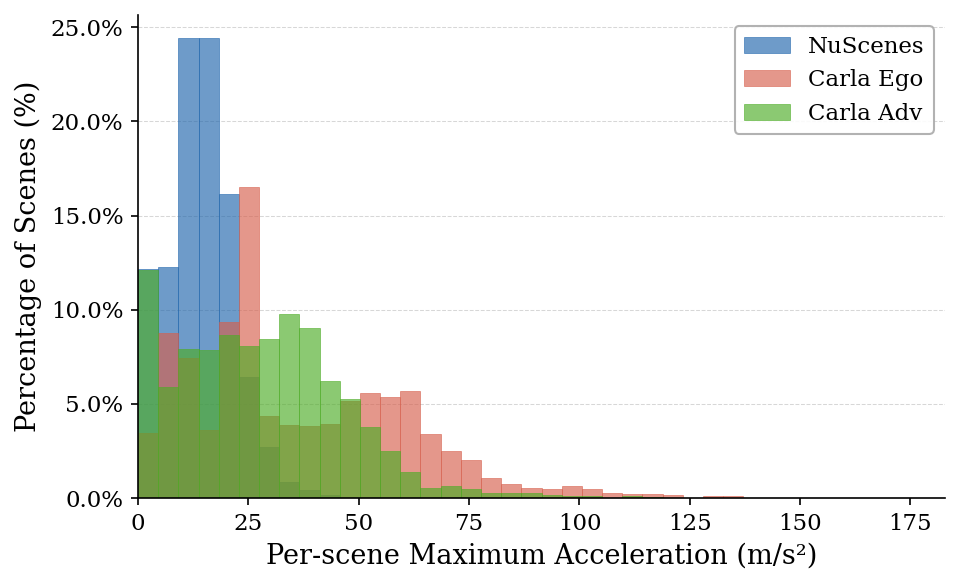
\includegraphics[width=0.6\linewidth]{figure/compare_ego_accel.png}
  \vskip -0.1in
  \caption{ 
  % Comparison of the maximum ego vehicle acceleration distribution in scenes from the CARLA Ego and nuScenes datasets. In the physically-challenging dataset, the ego vehicle's maximum acceleration is much higher than the nominal ego vehicle's maximum acceleration.
Distributions of maximum ego-vehicle acceleration for \textit{nuScenes}, \textit{CARLA Ego}, and \textit{CARLA ADV}. The simulated CARLA datasets show a clear shift toward higher accelerations, indicating more aggressive dynamics and physically challenging events compared with the predominantly nominal driving behaviors in \textit{nuScenes}.
  }
  \label{fig:compare_ego_accel}
  \vskip -0.1in
\end{figure}


\begin{figure}[tb]
  \centering
  \includegraphics[width=\linewidth]{figure/6dof-head_v4.pdf}
  \vskip -0.1in
  \caption{ 
  Comparison of MLP and time-wise output head in simulating collision dynamics. The MLP shows a gradual velocity decrease after the collision, while the GT and time-wise head show an instantaneous drop to zero, producing more realistic dynamics.
  }
  \vskip -0.1in
  \label{fig:6dof-head}
\end{figure}



\noindent \textbf{Architecture.} The architecture of the physical model is illustrated in the left of Figure \ref{fig:framework} (b). For a given scenario, the input trajectories $\mathcal{T}^{orig}$ are encoded via sine--cosine positional encoding followed by an MLP encoder into agent tokens $\mathbf{q} \in \mathbb{R}^{N \times D}$, where $N$ denotes the number of agents and $D$ is the token dimension. To ensure that these agents interact reasonably with the visual environment, we first apply deformable spatial cross-attention to interact with the multi-view Perspective View (PV) features $\mathcal{F}_{pv}$ based on their trajectory coordinates. This operation yields the spatially grounded queries $\mathbf{q}_{s}$:
\begin{equation}
    \mathbf{q}_{s} = \text{SpatialCrossAttn}(\mathbf{q}, \mathcal{F}_{pv})
\end{equation}
Subsequently, an agent-agent self-attention layer is introduced to enable the tokens to perceive the positional and kinematic states of surrounding vehicles, which is the key design for resolving overlapping and penetration conflicts:
\begin{equation}
    \mathbf{q}_{a} = \text{AgentSelfAttn}(\mathbf{q}_{s})
\end{equation}
Furthermore, a map cross-attention layer integrates vectorized map embeddings $\mathbf{E}_{map}$ for better off-road awareness:
\begin{equation}
    \mathbf{q}_{m} = \text{MapCrossAttn}(\mathbf{q}_{a}, \mathbf{E}_{map})
\end{equation}
Finally, a Feed-Forward Network is applied to non-linearly transform the aggregated features, yielding the fully refined queries $\mathbf{q}_{f}$ before trajectory prediction:
\begin{equation}
    \mathbf{q}_{f} = \text{FFN}(\mathbf{q}_{m})
\end{equation}

% To ensure that these agents interact reasonably with both the visual environment, we first apply deformable spatial cross-attention to interact with the multi-view Perspective View (PV) features $\mathcal{F}_{pv}$ based on their trajectory coordinates:
% \begin{equation}
%     \mathbf{q}^{(l, 1)} = \mathbf{q}^{(l-1)} + \text{SpatialCrossAttn}(\mathbf{q}^{(l-1)}, \mathcal{F}_{pv})
% \end{equation}
% Subsequently, an agent-agent self-attention layer is introduced to enable the tokens to perceive the positional and kinematic states of surrounding vehicles, which is the key design for resolving overlapping and penetration conflicts:
% \begin{equation}
%     \mathbf{q}^{(l, 2)} = \mathbf{q}^{(l, 1)} + \text{AgentSelfAttn}(\mathbf{q}^{(l, 1)})
% \end{equation}
% Furthermore, a map cross-attention layer integrates vectorized map embeddings $\mathbf{E}_{map}$ for better off-road awareness:
% \begin{equation}
%     \mathbf{q}^{(l, 3)} = \mathbf{q}^{(l, 2)} + \text{MapCrossAttn}(\mathbf{q}^{(l, 2)}, \mathbf{E}_{map})
% \end{equation}
% Finally, a Feed-Forward Network (FFN) is applied to non-linearly transform the aggregated features, enhancing the representation capacity of the refined queries before trajectory prediction:
% \begin{equation}
%     \mathbf{q}^{(l)} = \mathbf{q}^{(l, 3)} + \text{FFN}(\mathbf{q}^{(l, 3)})
% \end{equation}


% To ensure that these agents interact reasonably with both the visual environment, we first apply deformable spatial cross-attention to interact with the multi-view Perspective View (PV) features based on their trajectory coordinates. Subsequently, an agent-agent cross-attention layer is introduced to enable the tokens to perceive the positional and kinematic states of surrounding vehicles, which is the key design for resolving overlapping and penetration conflicts. Furthermore, a map cross-attention layer integrates vectorized map embeddings for better off-road awareness. 随后一个FFN被添加用来干啥（这个你要自己想）.


Following the above layers, the refined queries need to be projected into the final trajectories. Traditional MLPs typically smooth out trajectory outputs, failing to capture the sudden, high-frequency dynamic impulses indicative of a collision. To address this, we specifically design a \textit{Time-Wise Output Head} as the final prediction module. For the $i$-th refined agent token $\mathbf{q}_f[i]$, we expand it across the $T$ future steps and concatenate it with a step-specific learnable temporal embedding $\mathbf{E}_{time}(t)$. The concatenated feature is then processed by a Temporal Convolutional Network (TCN) to capture local inter-step dynamic variations, before being projected by an MLP to output the exact 6-DoF state:
\begin{equation}
    \mathbf{h}_{i,t} = \text{TCN} \left( \text{Proj}(\mathbf{q}_f[i] \parallel \mathbf{E}_{time}(t)) \right)
\end{equation}
\begin{equation}
    \hat{\mathcal{T}}_{i,t}^{6dof} = \text{MLP}(\mathbf{h}_{i,t}) \in \mathbb{R}^6
\end{equation}
As shown in Figure~\ref{fig:6dof-head}, unlike standard regression heads that produce sluggish responses, this time-wise formulation paired with step-specific time embeddings accurately captures the abrupt physical changes at the physical impact moment.


% Following the above layers, the refined tokens need to be projected into the final trajectories. Traditional MLPs typically smooth out trajectory outputs, failing to capture the sudden, high-frequency dynamic impulses indicative of a collision. To address this, we specifically design a \textit{Stepwise 6-DoF Head} as the final prediction module. For the $i$-th refined agent token $\mathbf{z}_i$, we expand it across the $T$ future steps and concatenate it with a step-specific learnable temporal embedding $\mathbf{E}_{time}(t)$. The concatenated feature is then processed by an emporal Convolutional Network (TCN) to capture local inter-step dynamic variations, before being projected by an MLP to output the exact 6-DoF state:
% \begin{equation}
%     \mathbf{h}_{i,t} = \text{TCN} \left( \text{Proj}(\mathbf{z}_i \parallel \mathbf{E}_{time}(t)) \right)
% \end{equation}
% \begin{equation}
%     \hat{\mathbf{y}}_{i,t}^{6dof} = \text{MLP}(\mathbf{h}_{i,t}) \in \mathbb{R}^6
% \end{equation}
% As shown in \ref{fig:6dof-head}, unlike standard regression heads that produce sluggish responses, this stepwise formulation paired with explicit time embeddings accurately captures the abrupt kinematic changes at the exact moment of physical impact.



\setlength{\parskip}{1pt}
\noindent \textbf{Training Pair Construction.}  To equip the Physical Condition Generator with the ability to rectify physics-violating trajectory conditions, we construct paired training data that maps \emph{physics-violating} trajectory inputs to physically feasible targets. To achieve this, we propose a systematic counterfactual trajectory corruption strategy. Specifically, for a collision clip in our simulated  dataset, we keep the original trajectory logs before the collision. For the post-collision frames, we intentionally corrupt the trajectories of all agents by extending their path with the same velocity before the collision, which synthesizes penetration-style counterfactual trajectory conditions. The ground-truth simulation logs---which capture the actual collision dynamics---serve as the supervision target for correction. In addition, to avoid distorting natural driving conditions, we also include real-world nominal trajectory-condition pairs from nuScenes without applying counterfactual corruption, ensuring the model preserves realistic inputs while learning to rectify physically invalid ones.


% 为了让这个physical condition generator能够具备物理感知调整不符合物理的轨迹，需要构建物理-violating的轨迹输入到符合物理的轨迹的训练数据对。 我们利用simulated 物理挑战数据并结合系统化的反事实轨迹制造策略来实现。 具体而言，. For a specific collision clip, we retain the original trajectory logs prior to the impact. However, for the post-impact frames, we artificially extrapolate the trajectories of all agents using a constant velocity linear motion model (这个不要用什么物理外推模型来写，就说碰撞后匀速直线外推). This effectively synthesizes a severe "penetration/counterfactual" input. The ground-truth simulation logs, which contain the true physical scatter dynamics, serve as the optimization target. 我们同样保留了Nuscenes中作为作为norminal轨迹条件下，不做反事实策略处理修改，的训练数据。防止将自然轨迹输入修改.


% Since ground-truth "counterfactual-to-physical" trajectory pairs do not exist in reality, we construct a synthetic fine-tuning dataset utilizing the collision events logged in our CARLA datasetNote that routine nuScenes data, which contains collision-free trajectories, is also preserved during training without modification. This ensures that the Physical Model retains the capability to faithfully output the original trajectories when the inputs are already physically plausible, preventing unnecessary alterations to nominal driving behaviors.



\setlength{\parskip}{1pt}
\noindent \textbf{Optimization.} The Physical Model is optimized using a weighted distance loss between the predicted 6-DoF trajectories and the ground truth:
\begin{equation}
    \mathcal{T}_{phy} = \frac{1}{N \times T} \sum_{i=1}^{N} \sum_{t=1}^{T} W_{i,t} \left\| \hat{\mathcal{T}}_{i,t}^{6dof} - \mathcal{T}_{i,t}^{gt} \right\|_1
\end{equation}
To focus on critical physical moments, we define $W_{i,t}$ with two scalars: an event-window weight $\lambda_{\text{event}}$ that increases the loss within a temporal window around collision/off-road timesteps, and a physical-agent weight $\lambda_{\text{agent}}$ that further amplifies the loss for agents involved in the interaction.

\subsection{Physics-Enhanced Multi-view Video Generator}
\label{Physics-Enhanced Multi-view Video Generator}

The second stage of our framework is the Physics-Enhanced Multi-View Video Generator (PE-MVGen). Built upon Wan2.1 \cite{wan2025wan}, a high-capacity diffusion transformer (DiT) originally conditioned on images and text, we adapt it into a controllable, multi-view generator explicitly designed for the autonomous driving domain. Crucially, this generator is endowed with deep physical awareness through a specialized heterogeneous co-training strategy.

\setlength{\parskip}{1pt}
\noindent \textbf{Multi-View~\& Layout Conditioning.} We first encode the input multi-view clips into latents $\mathbf{z}\in\mathbb{R}^{V\times T\times C\times h\times w}$ using a pre-trained 3D VAE~\cite{wan2025wan}, where $V$ represents the number of views. To enable multi-view modeling without introducing additional parameters \cite{gao2025magicdrive,wen2024panacea}, we reshape the input into $ T\times C\times h \times ( V \cdot w) $, concatenating the view dimension into the spatial axis so that the same self-attention can capture cross-view dependencies. Furthermore, to explicitly condition generation on structural layouts, we project the future $T$-frame 3D agent boxes and map polylines onto each camera view using the calibrated intrinsics $\mathbf{K}_v$ and extrinsics $\mathbf{E}_v$. The resulting view-specific control images $\mathbf{M}_v$ are encoded by the VAE encoder to get $\mathbf{z}_c$ , reshaped to match the video latents, concatenated along the channel dimension with the noisy latent input $\mathbf{z}_t$, and finally processed by a patch embedder before entering the DiT.

\setlength{\parskip}{1pt}
\noindent \textbf{Data-Driven Physical Enhancement.} Current world models fail in physically challenging scenarios because their training distributions lack physical interactions. To solve this, we train PE-MVGen on our heterogeneous dataset, maintaining a balanced 1:1 ratio between nominal real-world logs and simulated physically challenging data. Crucially, we do not use counterfactual trajectories at this stage; the generator is supervised with ground-truth physical trajectories, decoupling physical correction from rendering. As demonstrated in Figure \ref{fig:with_physical_data}, co-training with this physics-rich data significantly enhances the model's physical understanding, allowing its generative capabilities to robustly generalize to physically challenging scenarios in real-world. \cite{ge2025unraveling,fang2025rebot}

\setlength{\parskip}{1pt}
\noindent \textbf{Training Objective.} Following Wan 2.1, PE-MVGen is optimized via Rectified Flows \cite{esser2024scaling}, which ensures stable training through ordinary differential equations (ODEs). During training, given a clean video latent $\mathbf{z}_1$, a random noise $\mathbf{z}_0 \sim \mathcal{N}(\mathbf{0}, \mathbf{I})$, and a timestep $t \in [0,1]$ sampled from a logit-normal distribution, the intermediate noisy latent $\mathbf{z}_t$ is defined as a linear interpolation:
\begin{equation}
    \mathbf{z}_t = t\mathbf{z}_1 + (1 - t)\mathbf{z}_0
\end{equation}
The ground-truth velocity vector is defined as $\mathbf{v}_t = \mathbf{z}_1 - \mathbf{z}_0$. The DiT model, parameterized by $\theta$, is trained to predict this velocity $u_\theta$. The flow-matching objective is formulated as the Mean Squared Error (MSE):
\begin{equation}
    \mathcal{L}_{FM} = \mathbb{E}_{\mathbf{z}_0, \mathbf{z}_1, t} \left\| u_\theta(\mathbf{z}_t, t, \mathbf{c}_{init}, \mathbf{c}_{text}, \mathbf{c}_{layout}) - \mathbf{v}_t \right\|_2^2
\end{equation}
where the predicted velocity $u_\theta$ is conditioned on three key components: $\mathbf{c}_{init}$ denotes the latent features of a single initial context frame, $\mathbf{c}_{text}$ represents the scene caption, and $\mathbf{c}_{layout}$ encodes the future multi-view layout images.

\setlength{\parskip}{1pt}
\noindent \textbf{Curriculum Co-Training Strategy.} We adopt a highly efficient two-stage curriculum: pre-training at a lower resolution ($224 \times 400$) to quickly learn multi-view geometry and physically challenging layout mappings, followed by high-resolution ($448 \times 800$) fine-tuning to ensure visual fidelity. 

% The second stage of our framework is the Physics-Enhanced Multi-view Video Generator (PE-MVGen). We start from Wan2.1 \cite{wan2025wan}, a 高质量diffusion transformer (DiT) originally conditioned on images and text. 我们将其adapt to a 多视角可控物理性增强的自动驾驶域生成器。



% 我们首先利用预训练的3D VAE提取latent 特征z ∈ RV×T×16×h×w from the input multiview video clip, where V represents the number of views, T
% denotes the sequence length of frames, h and w denote the
% height and width of the latent features, respectively. 随后为了实现多视角建模，Unlike，额外引入的提高训练负担的cross-view attention module，我们follow dive，drivedreamer的方式，将 reshaping the input from B × V ×T ×H′ ×W′ × CtoB × T × ×KW × CandtreatingVH′W′ as the sequence length. 不引入额外参数，利用模型原有的子注意力模块建模多视角信息交互。随后为了实现map和box控制，我们将未来T帧的结构化layout信息（agent3D box与lane）投影到V个视角的相机平面中利用。calibrated intrinsics Kv and extrinsics Ev , resulting in a set of view-specific semantic control maps Mv ∈ RH×W ×3*T . These projected maps—comprising layout curves, pose skeletons, and instance masks—are subsequently encoded with VAE encoder \cite{}
% 成与训练视频片段相同shape后同样reshape 成相同的 B × T × ×KW × C 后与noised视频输入concat，最后再通过一个patch embedder. 后给到dit进行训练。

% 为了提高视频生成模型在物理挑战场景下的生成能力，我们的认为必须利用包含物理交互的数据进行训练，为此我们利用了我们的混合数据集作为dit的训练数据，其中norminal 自然数据和仿真物理挑战数据约为1：1。 我们在训练生成模型时没有使用反事实轨迹制造策略，而是利用数据集的准确轨迹来引导生成，将物理修正与渲染能力解耦处理。我们发现通过结合这种训练数据能显著提高的理解能力，如图4所示，模型可以泛化到真实域下的物理挑战场景下的生成能力大幅度提高。


% \textbf{Training Objective.} The PGMVM is optimized using the standard flow-matching/diffusion loss:
% \begin{equation}
%     \mathcal{L}_{diffusion} = \mathbb{E}_{\mathbf{x}, \epsilon, t} \left\| \mathbf{x} - \mathcal{D}_\theta (\mathbf{x}_t; t, \mathbf{h}_{prev}, \mathbf{c}_{text}, \mathbf{c}_{layout}) \right\|_2^2
% \end{equation}
% where $\mathbf{x}$ is the clean video latent, $\mathbf{x}_t$ is the noisy latent at timestep $t$, and $\mathcal{D}_\theta$ is the DiT parameterized by $\theta$. The model is explicitly conditioned on the historical context frames $\mathbf{h}_{prev}$, text descriptions $\mathbf{c}_{text}$, and the physical layout $\mathbf{c}_{layout}$

%这一段要参考：Training objective. Flow matching provides a theoretically grounded framework for learning continuous-time generative processes in diffusion models. It circumvents iterative velocity prediction, enabling stable training via ordinary differential equations (ODEs) while maintaining equivalence to maximum likelihood objectives. During training, given an image or video latent x1, a random noisex0 ∼ N (0, I), and a timestep t ∈ [0, 1] sampled from a logit-normal distribution, an intermediate latent xt is obtained as the training input. Following Rectified Flows (RFs) (Esser et al., 2024), xt is defined as a linear interpolation between x0 and x1, i.e.,xt = tx1 + (1 − t)x0. (1) The groud truth velocity vt isvt = dxtdt = x1 − x0. (2) The model is trained to predict the velocity, thus, the loss function can be formulated as the mean squared error (MSE) between the model output and vt, 14 L = Ex0,x1,ctxt,t||u(xt, ctxt, t; θ) − vt||2, (3) where ctxt is the umT5 text embedding sequence of 512 tokens long, θ is the model weights, andu(xt, ctxt, t; θ) denotes the output velocity predicted by the model.的内容来写，这个是原本wan的train objective

% \textbf{Curriculum Co-Training Strategy.} We employ a two-stage curriculum training strategy using the heterogeneous data compilation. We first pre-train the model on a lower resolution ($224 \times 448$ per view) until convergence to establish a foundational understanding of multi-view geometry and basic physical interactions. Subsequently, we fine-tune the model at a higher resolution ($448 \times 800$ per view). This pipeline produces a robust generator capable of synthesizing 3 seconds of 12Hz video, conditioned seamlessly on a single initial frame and the physically rectified layout.  这一段需要简单的说，并且把224*400上训练为了学习多视角集合和物理挑战控制条件输入，然后在高分辨率上保证高质量画面，这一段内容要少一点


% \section{Experiment}
% \subsection{Experimental Setup}
% \textbf{Datasets:} Training and evaluation are conducted on the nuScenes dataset and 我们的物理challenging 数据集, which includes 1,000 urban driving scenes (700 train / 150 val / 150 test). 

% 由于大多数世界模型都在真实域上进行训练，为此我们训练了一个风格迁移diffusion模型，我们用depth-anything-v2得到图像的深度信息，并使用qwen2.5VL 配合特定的prompt得到场景描述，并利用逐帧的深度信息作为condition，训练wan2.1模型，我们在训练过程中只是用Nuscenes图像。训练好了以后，我们将CARLA的测试集转换为偏nuscenes风格域进行测试, 作为视频生成的条件输入，与fid和fvd的计算GT。


% \textbf{Evaluation Metrics:}
% 我们从生成视频的可控性，物理性，视觉质量几个维度进行评估。与之前工作类似，我们使用fid和fvd来计算视频的画面的realism。对于物理性评估，我们使用world model bench进行评估，这个benchmark利用人类偏好对齐的VLM judges the world modeling capability of video generation models across diverse application-driven domains，我们将其中的Mass (objects do not irregularly deform or distort.), Penetration（Objects does not unnaturally pass through each other.）, Framewise quality(there is no visually unappealing frames or low-quality content.),temporal quality (there is no noticeable flickering, choppy motion, or abrupt appearance (disappearance) of irrelevant objects.)， 得分构成一个平均值。对于视频生成的可控性，我们使用streampetr评估mAP，并使用VIPE对模型的控制性做了一个评估。我们using Rotation Error (RotErr) and Translation Error (TransErr) metrics following previous works (cameractrl, cameractrl). ii). 相机的pose估计是使用VIPE.

% \textbf{Baseline: }
% 我们比较了三个baseline, Magicdrivev2, Unimlvg, dist-4d, 在我们评估数据集上的表现，我们均采用各自官方的实现，对于前两个方法以及我们的方法，利用的输入包含了初始帧画面以及生成时间未来的数据集标注信息，对于dist-4d，除了初始帧画面，还需要初始帧的深度信息，提供了额外的信息量。我们依照各自代码官方的代码进行预处理和视频生成。


% \textbf{Implement Details: }
% 我们的physical model的训练是在12hz数据上进行训练T=36，perception 特征使用 diffusiondrive预训练模型，训练期间冻结，N=2，Wi,t设置为1. 我们的视频生成模型主要使用wan2.1 vae，我们训练的帧长度是224*800,learning rate是5e-5，训练了2850step，第二阶段在448*800分辨率上训练，learning rate 为1e-5，训练了 1000 step. 我们的实验在64张V20上进行. 模型的输出是33帧.




\section{Experiment}
\subsection{Experimental Setup}
\textbf{Datasets:} We use the heterogeneous multi-view dataset introduced in Section~\ref{Heterogeneous Data}, including \textit{CARLA Ego}, \textit{CARLA ADV}, and \textit{nuScenes}, for training and evaluation. During training, we adopt balanced sampling to keep the simulated-to-real clip ratio close to 1:1. For video generation evaluation, we randomly sample 150 clips per test split and generate videos for all sampled clips. Since the compared baselines are primarily trained on \textit{nuScenes}, we translate the CARLA clips into the \textit{nuScenes} visual style using a learned style-transfer model (details in the supplementary material) for fair evaluation.

% We train our models on the heterogeneous dataset introduced in Section~\ref{Heterogeneous Data}. Specifically, we split \textit{CARLA-Ego} and \textit{CARLA-Adv} into training and test sets with a 7:1 ratio, and mix the resulting CARLA training subsets with the nuScenes training split for joint training. For video generation evaluation, we randomly sample 150 clips from each of the \textit{CARLA-Ego} test set, \textit{CARLA-Adv} test set, and the nuScenes validation split, and generate videos for all sampled clips.

% we use CARLA Ego，CARLA-adv，nuscenes introduced in section 3.2 for traing and testing. For training, we
%  split the heterogeneous dataset into 7:1, 用7份做训练， for video generation evaluation，我们randomly sample 150 clips from each of the dataset （这个要说明是每个数据集150个，隐式一点的说） to generate. 由于我们对比的baseline主要在nusceens上进行训练，因此我们使用一个风格迁移模型（detailed in Appendix）将CARLA数据迁移到nuscenes风格进行评估.

% Training and evaluation are conducted on the nuScenes \cite{caesar2020nuscenes} dataset and our physics-challenging CARLA dataset. We use the nuScenes dataset for normal driving scenarios and the physics-challenging CARLA dataset to simulate extreme physical interactions, such as collisions and off-road departures. 

% Since most world models are trained on real-world domains, we also train a style transfer diffusion model based on wan2.1 \cite{wan2025wan}. 针对一段视频，我们利用Qwen2.5VL给出详细的scene caption，并使用depth-anything-v2得到视频中逐帧的深度图. 随后我们在nuscenes数据集上利用深度图和scene caption作为条件输入上训练了一个根据文本描述和深度信息生成nuscenes风格域的风格迁移模型. 随后，我们利用该模型将仿真的物理挑战CARLA 数据集 风格迁移成nuscenes-like appearance;  these translated videos are used as the ground truth for FID/FVD computation, and their first frames are further extracted as the conditioning inputs for evaluating our video generation model.

% Since most driving world models are trained in real-world domains, we additionally train a diffusion-based style transfer model built upon Wan2.1 \cite{wan2025wan} to mitigate the sim-to-real appearance gap. For each video clip, we use Qwen2.5VL to produce a detailed scene caption, and extract frame-wise depth maps with Depth-Anything-v2. We then train the style transfer model on nuScenes dataset, conditioning on both the scene caption and per-frame depth to synthesize videos in a nuScenes-like visual style. After training, we apply this model to our physics-challenging CARLA dataset to translate simulated clips into a nuScenes-like appearance; these translated videos serve as the ground truth for FID/FVD computation, and we further extract their first frames as conditioning inputs when evaluating our video generation model.

% Since a noticeable domain gap exists between real-world nuScenes and simulated CARLA, we translate the CARLA test set into the nuScenes visual domain to ensure a fair comparison with world models trained on real data. Specifically, we train a nuScenes style transfer model on nuScenes videos, conditioning on frame-wise depth maps and detailed textual scene descriptions (details in the supplementary material), and apply it to convert our CARLA Ego and CARLA ADV test clips into a nuScenes-like appearance. These translated videos are treated as the ground truth for FID/FVD computation, and their first frames are further extracted as the conditioning inputs when evaluating the video generation model.


% We use depth information from Depth-Anything-v2 and scene descriptions from Qwen2.5VL with specific prompts. The model was trained on nuScenes images, and during training, we used frame-by-frame depth information as conditioning input. After training, we apply it to the CARLA test set to render CARLA sequences in a nuScenes-like appearance; these translated videos are used as the ground truth for FID/FVD computation, and their first frames are further extracted as the conditioning inputs for evaluating our video generation model.

% \noindent \textbf{Evaluation Metrics:}  
% We evaluate the generated videos along three dimensions: visual quality, physical plausibility, and controllability. Following prior work, we use FID and FVD to measure the realism of generated videos. \textbf{1.} For physical plausibility, we adopt WorldModelBench \cite{li2025worldmodelbench}, a 可以有效衡量自动驾驶视频生成效果的benchmark using human preference-aligned VLM-based judges. \textbf{2.} We report PHY as the average of four WorldModelBench metrics: Mass (objects do not deform or distort irregularly), Penetration (这个penetration换一个正向的词或者中兴的) (objects do not unnaturally pass through each other), Framewise Quality (no unappealing frames or low-quality content), and Temporal Quality (no noticeable flickering, choppy motion, or abrupt appearance/disappearance of irrelevant objects) (这个太长了少一点，就说与时间维度相关的一句解释就行了). \textbf{3.} For controllability, 这个要解释可控性衡量的是什么（轨迹layout条件下） we utilize Controllability Error (CtrlErr) metric to measure the difference between the trajectory extracted from generated videos and the real trajectory., which is the geometric mean of Rotation Error (RotErr) and Translation Error (TransErr), following previous works \cite{he2024cameractrl} \cite{duan2025worldscore}. Camera pose sequences are extracted using ViPE \cite{huang2025vipe}.

\setlength{\parskip}{1pt}
\noindent \textbf{Evaluation Metrics:}  
We evaluate generated videos along three dimensions: visual quality, physical plausibility, and controllability. \textbf{(1):} Following prior work, we use \textbf{FID} and \textbf{FVD} to measure the realism. 
 \textbf{(2):} For physical plausibility, we adopt WorldModelBench \cite{li2025worldmodelbench}, a benchmark that can effectively measure the effectiveness of autonomous driving video generation using human preference-aligned VLM-based judges.  We report \textbf{PHY} as the average of four WorldModelBench metrics: Mass (objects do not deform irregularly), Impenetrability (objects do not unnaturally pass through each other), Frame-wise Quality (no unappealing frames or low-quality content), and Temporal Quality (no temporally inconsistent scenes and objects).  In addition, we report a human preference rate (\textbf{Pref.}), computed as the percentage of pairwise comparisons in which a method is preferred by human annotators. Detailed questionnaire and settings are provided in the supplementary material. \textbf{(3):} For controllability, we measure how well the generated videos follow the input trajectory conditions. Specifically, we compute the Controllability Error (\textbf{CtrlErr}) between the trajectories extracted from generated videos and the ground-truth trajectories, defined as the geometric mean of Rotation Error and Translation Error, following prior work\cite{he2024cameractrl,duan2025worldscore}. Camera pose sequences are extracted using ViPE\cite{huang2025vipe}. 

\setlength{\parskip}{1pt}
\noindent \textbf{Baseline:}  
We compare our method with three baselines:  UniMLVG \cite{chen2025unimlvg}, MagicDrive-V2 \cite{gao2025magicdrive}, and DiST-4D \cite{guo2025dist}, evaluating their performance on our dataset. For UniMLVG, MagicDrive-V2, and our framework, the input includes the initial RGB frame, the scene captions, and future layout information. For DiST-4D, it additionally requires the initial-frame depth map alongside the initial RGB frame, providing extra geometric cues. Implementation details of these baselines are provided in the supplementary material.

\setlength{\parskip}{1pt}
\noindent \textbf{Implementation Details:}  
% The training of our Physical Model is conducted on 12Hz data with $T = 36$. Perception view features 利用resnet50的网络提取, which is training with learning rate 9e-5. 主干网络以9e-4的学习率学习. batchsize为256. We set $N = 2$ and $W_{i,t} = 1$. Our video generation model is based on the WAN2.1 预训练权重, with frame dimensions of $224 \times 400$. The learning rate is set to $5 \times 10^{-5}$, and we train for 2,850 steps. In the second stage, we train at a resolution of $448 \times 800$ with a learning rate of $1 \times 10^{-5}$ for 1,000 steps. All experiments are conducted on 64 V100 GPUs. The output of the model is 33 frames per video 12hz.
% The training of our Physical Condition Generator is conducted on 12Hz data with $T=36$. Perception-view features are extracted using a ResNet50 network trained with a learning rate of $9 \times 10^{-5}$. The backbone network is trained with a learning rate of $9 \times 10^{-4}$, and the batch size is set to 256. We set $N=2$ and $W_{i,t}=1$. For the weighted loss in \cref{eq:phy_loss}, we set the event-window weight $\lambda_{\text{event}}=10$ and the physical-agent weight $\lambda_{\text{agent}}=5$; an ablation over these hyperparameters is provided in the supplementary material.
The training of our Physical Condition Generator conducted on 12Hz data with $T=36$. Perception-view (PV) features are extracted using a ResNet50 \cite{he2016deep} initialized from \cite{sun2025sparsedrive} and trained with a learning rate of $9 \times 10^{-5}$. The main network is trained with a learning rate of $9 \times 10^{-4}$, and the batch size is set to 256. We set $N=2$ and for the loss weight $W_{i,t}$  in Section \ref{Physical condition generator}, we set $\lambda_{\text{event}}=10$ and $\lambda_{\text{agent}}=5$; an ablation over these hyperparameters is provided in the supplementary material.

% Our video generation model is based on the pre-trained WAN2.1 weights. The learning rate is set to \( 5 \times 10^{-5} \) of
%  the first , and we train the model for 2,850 steps  with a global batch size of 48. In the second stage, we train at a high resolution  with a learning rate of \( 1 \times 10^{-4} \) for 350 steps with global batchsize of 240. All experiments Training is performed with PyTorch using 48 NVIDIA H20 GPUs. The output of the model consists of 33 frames per video, at 12Hz. We employ the AdamW optimizer

Our video generation model is initialized from the pre-trained WAN2.1 weights and optimized with AdamW. We adopt a two-stage schedule: Stage~1 trains at $224\times 400$ for 2{,}850 steps with a learning rate of $5\times 10^{-5}$ and a global batch size of 480, followed by Stage~2 at $448\times 800$ for 350 steps with a learning rate of $1\times 10^{-4}$ and a global batch size of 240. Training is implemented on 48 NVIDIA H20 GPUs. The model generates 33-frame videos at 12\,Hz.


\subsection{Performance of PhyGenesis}\label{exp:complete framework}
% 在本章节中我们按照我们4.1的设定：即输入场景中车辆的2D未来轨迹的方式进行测试，对于Nuscenes数据模型的输入是原有的GT轨迹，但是只保留了x，y 2维数据，对于CARLA Ego和CARLA ADV数据，我们采取在发生碰撞后以碰撞前的速度保持匀速直线匀速外推轨迹的方式模拟反事实轨迹。对于baseline 方法我们额外补充了根据x增量和y 增量计算了yaw角用以模拟车辆旋转。定性结果如图4所示。实验结果如表1所示。

\vskip -0.1in
\begin{figure}[tb]
  \centering
  \includegraphics[width=\linewidth]{figure/baseline_2d_v9.pdf}
  \vskip -0.1in
  \caption{ 
  % Qualitative comparison with different baselines. Our method maintains the best physical consistency and visual quality, while other baselines exhibit deformation or object disappearance.
  Qualitative comparison with different baselines. Our method maintains the best physical consistency and produces the best visual quality.
  }
  \vskip -0.1in
  \label{fig:basline_2d_2}
\end{figure}




\begin{figure}[tb]
  \centering
  \includegraphics[width=\linewidth]{figure/Nuscenes-collision_v9.pdf}
  \vskip -0.1in
  \caption{ 
  Qualitative comparison on the \textit{nuScenes} stress test under out-of-distribution (OOD), physics-violating trajectory inputs, with the first-frame condition kept unchanged. 
  % Our method remains physically consistent, while other baselines exhibit deformation artifacts.
 Our method outperforms baselines with
  respect to physical consistency.
  }
  \label{fig:nuscenes-collision}
  \vskip -0.1in
\end{figure}


% \begin{table}[t]
% %\vskip -0.1in
% \caption{Performance comparison of our complete framework with baselines on the Nuscenes, CARLA Ego, and CARLA ADV datasets. The best performance is marked in bold.}
% \label{tab:performance_complete}
% %\vskip 0.1in
% \begin{center}
% \begin{small}
% \begin{sc}
% \resizebox{\columnwidth}{!}{%
% \begin{tabular}{l c ccc ccc ccc}
% \toprule
% \multirow{2}*{\textbf{Methods}} & \multirow{2}*{\textbf{Gen. Cond.}} &
% \multicolumn{3}{c}{Nuscenes} & \multicolumn{3}{c}{CARLA Ego} & \multicolumn{3}{c}{CARLA ADV} \\
% \cmidrule(lr){3-5} \cmidrule(lr){6-8} \cmidrule(lr){9-11}
% & & FID$\downarrow$ & FVD$\downarrow$ & PHY$\uparrow$
%   & FID$\downarrow$ & FVD$\downarrow$ & PHY$\uparrow$
%   & FID$\downarrow$ & FVD$\downarrow$ & PHY$\uparrow$ \\
% \midrule
% MagicDriveV2   & Init RGB         & 13.40 & 91.10 & 0.92 & 32.19 & 207.64 & 0.60 & 32.82 & 222.55 & 0.66 \\
% Dist-4D        & Init RGB + Depth & 10.49 & 46.95 & 0.86 & 19.84 & 197.57 & 0.39 & 16.07 & 128.88 & 0.56 \\
% UniMLVG        & Init RGB         & ---   & ---    & ---  & ---   & ---    & ---  & ---   & ---    & ---  \\
% Ours  & Init RGB         & \textbf{10.24} & \textbf{40.41}  & \textbf{0.97} & \textbf{11.03} & \textbf{72.48} & \textbf{0.71} & \textbf{9.28} & \textbf{77.83} & \textbf{0.87} \\
% \bottomrule
% \end{tabular}}
% \end{sc}
% \end{small}
% \end{center}
% %\vskip -0.3in
% \end{table}

\begin{table}[t]

\caption{Comparison with baselines under 2D trajectory conditions: \textit{nuScenes} uses nominal trajectories, while \textit{CARLA Ego} and \textit{CARLA ADV} use physics-violating trajectories. We report visual quality (FID/FVD), physical consistency (PHY), human preference (Pref.). PhyGenesis achieves the best results across all datasets.}
\vskip -0.15in
\label{tab:performance_complete}
%\vskip 0.1in
\begin{center}
\begin{small}
\begin{sc}
\resizebox{\columnwidth}{!}{%
\begin{tabular}{l c cccc cccc cccc}
\toprule
\multirow{2}*{\textbf{Methods}}&
\multicolumn{4}{c}{nuScenes} & \multicolumn{4}{c}{CARLA Ego} & \multicolumn{4}{c}{CARLA ADV} \\
\cmidrule(lr){2-5} \cmidrule(lr){6-9} \cmidrule(lr){10-13}
& FID$\downarrow$ & FVD$\downarrow$ & PHY$\uparrow$  & Pref. $\uparrow$
  & FID$\downarrow$ & FVD$\downarrow$ & PHY$\uparrow$ & Pref. $\uparrow$
  & FID$\downarrow$ & FVD$\downarrow$ & PHY$\uparrow$ & Pref. $\uparrow$ \\
\midrule
UniMLVG  \cite{chen2025unimlvg}             & 17.59   & 129.69    & 0.93 & 0.05 & 34.50   & 260.21    & 0.55 & 0.13 & 30.32   & 274.94    & 0.70 & 0.19 \\
MagicDrive-V2 \cite{gao2025magicdrive}        & 13.40 & 91.10 & 0.92& 0.16 & 32.19 &  207.64 & 0.60 & 0.06& 32.82 & 222.55 & 0.66 & 0.10 \\
DiST-4D \cite{guo2025dist}        & 10.49 & 46.95 & 0.86&  0.13 & 19.84 & 197.57 & 0.39 & 0.10& 16.07 & 128.88 & 0.56 & 0.05\\
PhyGenesis        & \textbf{10.24} & \textbf{40.41}  & \textbf{0.97} & \textbf{0.67} & \textbf{11.03} & \textbf{72.48}  & \textbf{0.71}& \textbf{0.71} & \textbf{9.28} & \textbf{77.83} & \textbf{0.87}& \textbf{0.66} \\
\bottomrule
\end{tabular}}
\end{sc}
\end{small}
\end{center}
\vskip -0.1in
\end{table}


% \begin{table}[t]
% \caption{Quantitative comparison of our complete PhyGenesis framework with state-of-the-art baselines on the nuScenes, CARLA Ego, and CARLA ADV datasets. The best performance is highlighted in \textbf{bold}.}
% \label{tab:performance_complete}
% \begin{center}
% \resizebox{\columnwidth}{!}{%
% \begin{tabular}{l ccc ccc ccc}
% \toprule
% \multirow{2}{*}{\textbf{Methods}} &
% \multicolumn{3}{c}{\textbf{nuScenes}} & \multicolumn{3}{c}{\textbf{CARLA Ego}} & \multicolumn{3}{c}{\textbf{CARLA ADV}} \\
% \cmidrule(lr){2-4} \cmidrule(lr){5-7} \cmidrule(lr){8-10}
% & \textbf{FID} $\downarrow$ & \textbf{FVD} $\downarrow$ & \textbf{Phy-Score} $\uparrow$
% & \textbf{FID} $\downarrow$ & \textbf{FVD} $\downarrow$ & \textbf{Phy-Score} $\uparrow$
% & \textbf{FID} $\downarrow$ & \textbf{FVD} $\downarrow$ & \textbf{Phy-Score} $\uparrow$ \\
% \midrule
% \makecell[l]{MagicDriveV2 \\ {[ICCV'25] \cite{xxx_magicdrive}}} 
% & 13.40 & 91.10 & 0.92 & 32.19 & 207.64 & 0.60 & 32.82 & 222.55 & 0.66 \\
% \addlinespace
% \makecell[l]{Dist-4D \\ {[ICCV'25] \cite{xxx_dist4d}}} 
% & 10.49 & 46.95 & 0.86 & 19.84 & 197.57 & 0.39 & 16.07 & 128.88 & 0.56 \\
% \addlinespace
% \makecell[l]{UniMLVG \\ {[CVPR'25] \cite{xxx_unimlvg}}} 
% & ---   & ---   & ---  & ---   & ---    & ---  & ---   & ---    & ---  \\
% \addlinespace
% \makecell[l]{\textbf{Ours}} 
% & \textbf{10.24} & \textbf{40.41} & \textbf{0.97} & \textbf{11.03} & \textbf{72.48} & \textbf{0.71} & \textbf{9.28} & \textbf{77.83} & \textbf{0.87} \\
% \bottomrule
% \end{tabular}%
% }
% \end{center}
% \end{table}

% \begin{table}[t]
% \caption{Physics score on the \textit{nuScenes} stress test with synthetically corrupted (physically-violating) trajectory conditions.}
% \label{tab:nuscenes_violation_phy}
% \begin{center}
% \begin{small}
% \begin{sc}
% \begin{tabular}{l c}
% \toprule
% \textbf{Method} & \textbf{Phy}$\uparrow$ \\
% \midrule
% MagicDriveV2 & 0.515 \\
% Dist-4D      & 0.6325 \\
% UniMLVG      & --- \\
% Ours         & \textbf{0.68} \\
% \bottomrule
% \end{tabular}
% \end{sc}
% \end{small}
% \end{center}
% \end{table}

% 我们首先按照Section 4.1所说的输入格式进行视频生成评估我们整体框架的表现. For the nuScenes dataset, the input 2D agent trajectories are equal to the ground-truth $(x, y)$ coordinates. For  CARLA Ego and CARLA ADV datasets, we corrupt the trajectories of all agents by extending their path with the velocity before the collision, which synthesizes physically-violating trajecotry conditions. To ensure a fair comparison, we augment the baseline methods by analytically (这个词能不能换成一个简单点的词) computing the vehicle yaw angles based on the spatial increments ($\Delta x, \Delta y$) to simulate rotation. .如Table \ref{tab:performance_complete}所示, 我们的模型在visual quality, physical score上全方面由于过往baseline. 在存在physically-violating的CARLA Ego和CARLA ADV 上提升非常明显, (分析). 定性的例子在 Figure \ref{fig:basline_2d_2}, 我们的方法生成的视频是physically-consistent的，另外的baseline出现变形.
% 为排除风格域带来的干扰，我们将nuscenes 测试集中下按规则放大自车速度制造physically-violating场景生成视频，定性和定量的例子可见fig:nuscenes-collision和table 5:

% We evaluate the full framework under the input protocol described in Section~4.1, where video generation is conditioned on future 2D agent trajectories. For the \textit{nuScenes} dataset, the trajectory condition is set to the ground-truth $(x,y)$ coordinates of all agents. For \textit{CARLA Ego} and \textit{CARLA ADV}, we synthesize physically-violating conditions by corrupting trajectories after the collision: we extrapolate each agent's post-impact motion using its pre-impact velocity with a constant-velocity straight-line extension. This creates severe counterfactual trajectory inputs while keeping the pre-collision segment unchanged. To ensure a fair comparison with prior diffusion baselines, we additionally provide approximate heading cues when required: we compute each vehicle's yaw from the 2D displacement increments $(\Delta x, \Delta y)$ (i.e., from the direction of motion) to emulate rotational motion. Qualitative examples are shown in Figure~\ref{fig:basline_2d_2}. As shown in Table~\ref{tab:performance_complete}, our method achieves the best physical consistency (Phy) across all datasets and also improves visual quality (FID/FVD) substantially on the physically-challenging CARLA settings. The gains are most pronounced on \textit{CARLA Ego} and \textit{CARLA ADV}, where the trajectory conditions are explicitly corrupted to violate collision physics: our physical -aware modeling better captures abrupt post-impact state changes (e.g., instantaneous velocity drops and realistic scattering), whereas prior diffusion baselines tend to smooth these discontinuities, often leading to stretched shapes, drifting agents, or temporally inconsistent motion.


% To further 证明我们框架在完全真实域的迁移能力, we additionally construct physically-violating conditions directly within the \textit{nuScenes} test set. Specifically, we modify the ego vehicle motion by scaling up its speed following a fixed rule, creating collision-prone and physically implausible trajectory conditions while keeping first frame condition unchanged. Figure~\ref{fig:nuscenes-collision} reports qualitative examples, and Table~\ref{tab:nuscenes_violation_phy} summarizes the physics scores. Our framework remains consistently more physically faithful under these corrupted conditions, indicating that the improvement is not merely due to domain/style differences but stems from stronger physical modeling.

% To further demonstrate that our framework generalizes to fully real-world data, we additionally construct physically-violating conditions directly within the \textit{nuScenes} test set. Specifically, we scale up the ego vehicle speed following a fixed rule to create collision-prone and physically implausible trajectory conditions, while keeping the first-frame conditioning unchanged. Figure~\ref{fig:nuscenes-collision} shows qualitative examples, and Table~\ref{tab:nuscenes_violation_phy} summarizes the physics scores. Our framework remains consistently more physically faithful under these corrupted conditions, highlighting its robustness to physically-violating trajectory inputs and its stronger capability of modeling physically-challenging dynamics.

% We evaluate the complete \textbf{PhyGenesis} framework under the trajectory-conditioning protocol described in Section~4.1. Specifically, generation is conditioned on future 2D agent trajectories. For \textit{nuScenes}, we directly use the ground-truth $(x,y)$ coordinate sequences as $\mathcal{T}_{1:T}^{orig}$. For \textit{CARLA Ego} and \textit{CARLA ADV}, we construct \textit{counterfactual} and \textit{physics-violating} trajectory conditions by corrupting the post-impact segment: we keep the original trajectories before the collision, but extend each agent's post-collision path using its pre-collision velocity with a constant-velocity straight-line extrapolation. For prior diffusion baselines, we further compute yaw angles from the spatial increments $(\Delta x, \Delta y)$ to simulate vehicle rotation, ensuring that all methods are evaluated with the same input trajectory format. Qualitative comparisons are shown in Figure~\ref{fig:basline_2d_2}. Table~\ref{tab:performance_complete} reports the quantitative results. Our framework achieves the best physical scores across all datasets, and also improves visual quality (FID/FVD) on the physically challenging \textit{CARLA Ego} and \textit{CARLA ADV} sets. The gains are most significant when the input trajectories are physics-violating: by rectifying counterfactual 2D inputs into physically plausible 6-DoF motions, our model avoids common failure patterns of prior methods, such as object deformation and implausible penetration under collision conditions. As illustrated in Figure~\ref{fig:basline_2d_2}, baseline generations often exhibit distorted structures or unrealistic interactions when forced to follow physics-violating trajectories, while our results remain physically consistent.

% To further demonstrate the transferability of our framework on fully real-world data, we additionally construct physics-violating conditions directly within the \textit{nuScenes} test set. Concretely, we scale up the ego vehicle speed following a fixed rule to create collision-prone and physically implausible trajectory conditions, while keeping the first-frame condition unchanged. Figure~\ref{fig:nuscenes-collision} shows qualitative examples, and Table~\ref{tab:nuscenes_violation_phy} summarizes the physics scores. \textbf{PhyGenesis} consistently achieves a higher Phy score under these corrupted conditions, indicating that our framework better maintains physically consistent generation when the input trajectories deviate from nominal driving.

In this section, we evaluate the effectiveness of \textbf{PhyGenesis}. For \textit{nuScenes}, we use the ground-truth $(x,y)$ trajectories as the input trajectory condition $\mathcal{T}^{orig}$. For \textit{CARLA Ego} and \textit{CARLA ADV}, to assess generation under physically-violating trajectory inputs, we construct counterfactual, physics-violating conditions following Section~\ref{Physical condition generator}: we keep the pre-collision trajectories unchanged and extrapolate the post-collision motion using each agent's pre-collision velocity. For baseline methods, we additionally compute yaw angles from $(\Delta x,\Delta y)$ to simulate rotation for a fair comparison~\cite{liao2025diffusiondrive}. As shown in Table~\ref{tab:performance_complete}, our framework achieves the best physical scores across all datasets and attains the best visual quality, with the largest gains on the physically challenging CARLA sets, , where physics-violating inputs often cause deformation and penetration in prior methods (Figure~\ref{fig:basline_2d_2}).

To evaluate video generation under out-of-distribution, physically challenging trajectories in real-world scenes, we additionally conduct a \textit{nuScenes} stress test. Specifically, we create physics-violating trajectory conditions in the \textit{nuScenes} test set by scaling up the ego vehicle speed and retaining only collision cases, while keeping the first-frame condition unchanged. Qualitative and quantitative results in Figure~\ref{fig:nuscenes-collision} and Figure~\ref{fig:nuscenes_violation_bar} show that \textbf{PhyGenesis} remains more physically consistent under these corrupted conditions.
% |  | physical score |
% | --- | --- |
% | magicdrive | 0.515 |
% | Dist4d | 0.6325 |
% | unimlvg | - |

% | Our framework | 0.68 |






% \begin{table}[t]
% %\vskip -0.1in
% \caption{Performance comparison of our complete framework with baselines on the Nuscenes, CARLA Ego, and CARLA ADV datasets. The best performance is marked in bold.}
% \label{tab:performance_complete}
% %\vskip 0.1in
% \begin{center}
% \begin{small}
% \begin{sc}
% \resizebox{\columnwidth}{!}{%
% \begin{tabular}{l c ccc ccc ccc}
% \toprule
% \multirow{2}*{\textbf{Methods}} & \multirow{2}*{\textbf{Gen. Cond.}} &
% \multicolumn{3}{c}{Nuscenes} & \multicolumn{3}{c}{CARLA Ego} & \multicolumn{3}{c}{CARLA ADV} \\
% \cmidrule(lr){3-5} \cmidrule(lr){6-8} \cmidrule(lr){9-11}
% & & FID$\downarrow$ & FVD$\downarrow$ & Phy-Score$\uparrow$
%   & FID$\downarrow$ & FVD$\downarrow$ & Phy-Score$\uparrow$
%   & FID$\downarrow$ & FVD$\downarrow$ & Phy-Score$\uparrow$ \\
% \midrule
% MagicDriveV2   & Init RGB              & 13.395 & 104.85   & 0.92 & 32.186 & 345.873 & 0.60 & 32.82  & 405.78  & 0.66 \\
% Dist-4D        & Init RGB + Depth & \textbf{10.489} & \textbf{59.196} & 0.86 & 19.841 & 168.51  & 0.39 & 16.067 & 151.838 & 0.56 \\
% UniMLVG        & Init RGB              & ---    & ---      & ---  & ---    & ---     & ---  & ---    & ---     & ---  \\
% Our Framework  & Init RGB              & 10.702 & 84.0701  & \textbf{0.97} & \textbf{12.018} & \textbf{112.149} & \textbf{0.70} & \textbf{9.880} & \textbf{103.379} & \textbf{0.87} \\
% \bottomrule
% \end{tabular}}
% \end{sc}
% \end{small}
% \end{center}
% %\vskip -0.3in
% \end{table}



% \begin{table}[t]
% \caption{Performance comparison of our complete framework with baselines. We report FID, FVD, and Phy-Score on each dataset, along with the average across the three datasets (Avg.). The best results are highlighted in \textbf{bold}.}
% \label{tab:performance_complete_vertical}
% \begin{center}
% \begin{small}
% \begin{sc}
% \resizebox{\columnwidth}{!}{%
% \begin{tabular}{llcccc}
% \toprule
% \textbf{Dataset} & \textbf{Metric} & \textbf{MagicDriveV2} & \textbf{Dist-4D} & \textbf{UniMLVG} & \textbf{Ours} \\
% \midrule
% \multirow{3}{*}{nuScenes}
% & FID$\downarrow$      & 13.40 & \textbf{10.49} & --- & 10.70 \\
% & FVD$\downarrow$      & 104.85 & \textbf{59.20} & --- & 84.07 \\
% & Phy-Score$\uparrow$  & 0.92 & 0.86 & --- & \textbf{0.97} \\
% \midrule
% \multirow{3}{*}{CARLA Ego}
% & FID$\downarrow$      & 32.19 & 19.84 & --- & \textbf{12.02} \\
% & FVD$\downarrow$      & 345.87 & 168.51 & --- & \textbf{112.15} \\
% & Phy-Score$\uparrow$  & 0.60 & 0.39 & --- & \textbf{0.70} \\
% \midrule
% \multirow{3}{*}{CARLA ADV}
% & FID$\downarrow$      & 32.82 & 16.07 & --- & \textbf{9.88} \\
% & FVD$\downarrow$      & 405.78 & 151.84 & --- & \textbf{103.38} \\
% & Phy-Score$\uparrow$  & 0.66 & 0.56 & --- & \textbf{0.87} \\
% \midrule
% \multirow{3}{*}{Avg.}
% & FID$\downarrow$      & 26.14 & 15.47 & --- & \textbf{10.87} \\
% & FVD$\downarrow$      & 285.50 & 126.52 & --- & \textbf{99.87} \\
% & Phy-Score$\uparrow$  & 0.73 & 0.60 & --- & \textbf{0.85} \\
% \bottomrule
% \end{tabular}}
% \end{sc}
% \end{small}
% \end{center}
% \end{table}

% \begin{table}[t]
% \caption{Performance comparison of our complete framework with baselines on nuScenes, CARLA Ego, and CARLA ADV. We additionally report Avg. as the macro-average over the three datasets. The best results are highlighted in \textbf{bold}.}
% \label{tab:performance_complete_dataset_method}
% \begin{center}
% \begin{small}
% \begin{sc}
% \resizebox{\columnwidth}{!}{%
% \begin{tabular}{llcccc}
% \toprule
% \textbf{Dataset} & \textbf{Method} & FID$\downarrow$ & FVD$\downarrow$ & Phy-Score$\uparrow$ & Human Study$\uparrow$ \\
% \midrule
% \multirow{4}{*}{nuScenes}
% & MagicDriveV2 & 13.40 & 104.85 & 0.92 & \\
% & Dist-4D      & \textbf{10.49} & \textbf{59.20} & 0.86 & \\
% & UniMLVG      & --- & --- & --- & \\
% & Ours         & 10.70 & 84.07 & \textbf{0.97} & \\
% \midrule
% \multirow{4}{*}{CARLA Ego}
% & MagicDriveV2 & 32.19 & 345.87 & 0.60 & \\
% & Dist-4D      & 19.84 & 168.51 & 0.39 & \\
% & UniMLVG      & --- & --- & --- & \\
% & Ours         & \textbf{12.02} & \textbf{112.15} & \textbf{0.70} & \\
% \midrule
% \multirow{4}{*}{CARLA ADV}
% & MagicDriveV2 & 32.82 & 405.78 & 0.66 & \\
% & Dist-4D      & 16.07 & 151.84 & 0.56 & \\
% & UniMLVG      & --- & --- & --- & \\
% & Ours         & \textbf{9.88} & \textbf{103.38} & \textbf{0.87} & \\
% \midrule
% \multirow{4}{*}{Avg.}
% & MagicDriveV2 & 26.14 & 285.50 & 0.73 & \\
% & Dist-4D      & 15.47 & 126.52 & 0.60 & \\
% & UniMLVG      & --- & --- & --- & \\
% & Ours         & \textbf{10.87} & \textbf{99.87} & \textbf{0.85} & \\
% \bottomrule
% \end{tabular}}
% \end{sc}
% \end{small}
% \end{center}
% \end{table}

\subsection{Performance of Physics-enhanced Multi-view Video Generator}

\begin{table}[t]
\vskip -0.1in
\caption{Comparison of video generators of different baselines under GT trajectory conditions. We report visual realism (FID/FVD), physical consistency (Phy), and controllability error (CtrlErr); best results are in \textbf{bold}.}
\vskip -0.1in
\label{tab:performance_video_generator}
\begin{center}
\begin{small}
\begin{sc}
\resizebox{\columnwidth}{!}{
\begin{tabular}{lcccccccccccccccc}
\toprule
\multirow{2}*{\textbf{Methods}} & \multicolumn{4}{c}{\textit{nuScenes}} & \multicolumn{4}{c}{\textit{CARLA Ego}} & \multicolumn{4}{c}{\textit{CARLA ADV}} \\
\cmidrule(lr){2-5} \cmidrule(lr){6-9} \cmidrule(lr){10-13}
& FID $\downarrow$ & FVD$\downarrow$  & PHY $\uparrow$  & CtrlErr $\downarrow$
& FID $\downarrow$  & FVD $\downarrow$  & PHY $\uparrow$ & CtrlErr $\downarrow$
& FID $\downarrow$  & FVD $\downarrow$  & PHY $\uparrow$ & CtrlErr $\downarrow$ \\
\midrule
UniMLVG \cite{chen2025unimlvg}       &  16.63   & 113.23    &  0.92 & 0.35  & 34.03 & 240.78  & 0.56    & 1.32  &  30.06 & 264.59 & 0.75   & 0.66     \\
MagicDrive-V2 \cite{gao2025magicdrive} & 13.17 & 88.86 & 0.93 & 0.29  & 32.92 & 181.26 & 0.58 & 1.26 & 33.62 & 214.52 & 0.65 & 0.75 \\
DiST-4D \cite{guo2025dist}     & 10.48 & 45.24 & 0.84 & 0.28 & 19.94 & 133.10 & 0.38 & 1.19 & 16.12 & 105.70 & 0.50 &  0.57\\
PhyGenesis & \textbf{10.20} & \textbf{31.14}  & \textbf{0.97} & \textbf{0.25}& \textbf{10.98} & \textbf{57.02} & \textbf{0.69} & \textbf{0.85}  & \textbf{9.07} & \textbf{59.44} & \textbf{0.83} & \textbf{0.37} \\
\bottomrule
\end{tabular}
}
\vskip -0.1in
\end{sc}
\end{small}
\end{center}
\end{table}

% 在本章节, 我们单独评估视频生成器的表现，我们利用数据集中的GT轨迹,（没有制造反事实轨迹），在nuscenes，CARLA Ego 和CARLA ADV数据集上进行实验，实验结果如表tab:performance_video_generator所示， （一段常规分析），要说其他baseline在面对符合无力的轨迹下因为缺少物理相关数据生成和控制性都更差

In this section, we evaluate the Physics-Enhanced Video Generator. We condition all methods on \emph{ground-truth} trajectories (i.e., no counterfactual or physics-violating inputs) and report results on \textit{nuScenes}, \textit{CARLA Ego}, and \textit{CARLA Adv} in Table~\ref{tab:performance_video_generator}. Although the inputs are physically feasible, prior baselines are trained mostly on nominal logs and rarely see physics-rich interactions (e.g., collisions and off-road events), so they still struggle to render these dynamics, resulting in worse visual quality, physical consistency, and controllability. In contrast, our PE-MVGen is co-trained with physics-rich data, better capturing complex interactions and improving both generation quality and condition following.

% \begin{table}[t]
% \caption{Performance comparison of video generation quality across different models, including FID, FVD, physical metrics, and error metrics on CARLA Ego and CARLA ADV datasets. The best performance is marked in bold.}
% \label{tab:performance_video_generator}
% \begin{center}
% \begin{small}
% \begin{sc}
% \resizebox{\columnwidth}{!}{
% \begin{tabular}{lcccccccccccccccc}
% \toprule
% \multirow{2}*{\textbf{Methods}} & \multicolumn{5}{c}{Nuscenes} & \multicolumn{5}{c}{CARLA Ego} & \multicolumn{5}{c}{CARLA ADV} \\
% \cmidrule(lr){2-6} \cmidrule(lr){7-11} \cmidrule(lr){12-16}
% & FID & FVD & Phy-Score& TransErr & RotErr & FID & FVD & Phy-Score & TransErr & RotErr & FID & FVD & Phy-Score & TransErr & RotErr \\
% \midrule
% MagicDriveV2 & 13.173 & 103.605 & 0.93 & \textbf{0.309} & 0.004 & 32.92 & 334.97 & 0.58 & 0.347 & 0.017 & 33.623 & 399.216 & 0.65 & 0.227 & 0.010 \\
% Dist-4D & \textbf{10.475} & \textbf{57.341} & 0.84 & 0.310 & 0.004 & 19.936 & 141.426 & 0.38 & 0.344 & 0.016 & 16.118 & 130.785 & 0.50 & \textbf{0.194} & 0.008 \\
% UniMLVG & —— & —— & —— & —— & —— & —— & —— & —— & —— & —— & —— & —— & —— & —— & ——  \\
% Our Framework & 10.53 & 73.033 & \textbf{0.97} & \textbf{0.309} & \textbf{0.003} & \textbf{12.077} & \textbf{86.394} & \textbf{0.69} & \textbf{0.303} & \textbf{0.012} & \textbf{9.608} & \textbf{76.768} & \textbf{0.82} & 0.202 & \textbf{0.006} \\
% \bottomrule
% \end{tabular}
% }
% \end{sc}
% \end{small}
% \end{center}
% \end{table}



% \begin{table}[t]
% \caption{Performance comparison of video generation quality across different models on nuScenes, CARLA Ego, and CARLA ADV. The best performance is marked in bold. TransErr and RotErr are reported with three decimal places due to their small magnitude.}
% \label{tab:performance_video_generator_rotated}
% \begin{center}
% \begin{small}
% \begin{sc}
% \resizebox{\columnwidth}{!}{%
% \begin{tabular}{llccccc}
% \toprule
% \textbf{Dataset} & \textbf{Method} &
% FID$\downarrow$ & FVD$\downarrow$ & Phy-Score$\uparrow$ & TransErr & RotErr \\
% \midrule
% \multirow{4}{*}{nuScenes}
% & MagicDriveV2 & 13.17 & 103.61 & 0.93 & \textbf{0.309} & 0.221 \\
% & Dist-4D      & \textbf{10.48} & \textbf{57.34} & 0.84 & 0.310 & 0.213 \\
% & UniMLVG      & --- & --- & --- & --- & --- \\
% & Ours         & 10.53 & 73.03 & \textbf{0.97} & \textbf{0.309} & \textbf{0.183} \\
% \midrule
% \multirow{4}{*}{CARLA Ego}
% & MagicDriveV2 & 32.92 & 334.97 & 0.58 & 0.347 & 0.952 \\
% & Dist-4D      & 19.94 & 141.43 & 0.38 & 0.344 & 0.899 \\
% & UniMLVG      & --- & --- & --- & --- & --- \\
% & Ours         & \textbf{12.08} & \textbf{86.39} & \textbf{0.69} & \textbf{0.303} & \textbf{0.713} \\
% \midrule
% \multirow{4}{*}{CARLA ADV}
% & MagicDriveV2 & 33.62 & 399.22 & 0.65 & 0.227 & 0.570 \\
% & Dist-4D      & 16.12 & 130.79 & 0.50 & \textbf{0.194} & 0.432 \\
% & UniMLVG      & --- & --- & --- & --- & --- \\
% & Ours         & \textbf{9.61} & \textbf{76.77} & \textbf{0.82} & 0.202 & \textbf{0.344} \\
% \midrule

% \multirow{4}{*}{\textbf{Avg.}}
% & MagicDriveV2 & 26.57 & 279.27 & 0.72 & 0.294 & 0.581 \\
% & Dist-4D      & 15.51 & 109.85 & 0.57 & 0.283 & 0.515 \\
% & UniMLVG      & --- & --- & --- & --- & --- \\
% & \textbf{Ours} & \textbf{10.74} & \textbf{78.73} & \textbf{0.83} & \textbf{0.271} & \textbf{0.413} \\

% \bottomrule
% \end{tabular}}
% \end{sc}
% \end{small}
% \end{center}
% \end{table}

% \begin{table}[t]
% \caption{Performance comparison of video generation quality across different models on nuScenes, CARLA Ego, and CARLA ADV. The best performance is marked in bold. TransErr and RotErr are reported with three decimal places due to their small magnitude.}
% \label{tab:performance_video_generator_rotated}
% \begin{center}
% \begin{small}
% \begin{sc}
% \resizebox{\columnwidth}{!}{%
% \begin{tabular}{llccccc}
% \toprule
% \textbf{Dataset} & \textbf{Method} &
% FID$\downarrow$ & FVD$\downarrow$ & Phy-Score$\uparrow$ & Control-Error \downarrow \\
% \midrule
% \multirow{4}{*}{nuScenes}
% & MagicDriveV2 & 13.17 & 103.61 & 0.93 & 0.261 \\
% & Dist-4D      & \textbf{10.48} & \textbf{57.34} & 0.84 & 0.257 \\
% & UniMLVG      & --- & --- & --- & --- \\
% & Ours         & 10.53 & 73.03 & \textbf{0.97}  & \textbf{0.238} \\
% \midrule
% \multirow{4}{*}{CARLA Ego}
% & MagicDriveV2 & 32.92 & 334.97 & 0.58  & 0.575 \\
% & Dist-4D      & 19.94 & 141.43 & 0.38 & 0.574 \\
% & UniMLVG      & --- & --- & --- & --- \\
% & Ours         & \textbf{12.08} & \textbf{86.39} & \textbf{0.69} & \textbf{0.465} \\
% \midrule
% \multirow{4}{*}{CARLA ADV}
% & MagicDriveV2 & 33.62 & 399.22 & 0.65  & 0.360\\
% & Dist-4D      & 16.12 & 130.79 & 0.50 & 0.289 \\
% & UniMLVG      & --- & --- & --- & ---  \\
% & Ours         & \textbf{9.61} & \textbf{76.77} & \textbf{0.82} & \textbf{0.264} \\
% \midrule

% \multirow{4}{*}{\textbf{Avg.}}
% & MagicDriveV2 & 26.57 & 279.27 & 0.72 & 0.399  \\
% & Dist-4D      & 15.51 & 109.85 & 0.57 & 0.373 \\
% & UniMLVG      & --- & --- & --- & --- \\
% & \textbf{Ours} & \textbf{10.74} & \textbf{78.73} & \textbf{0.83} & \textbf{0.322}  \\

% \bottomrule
% \end{tabular}}
% \end{sc}
% \end{small}
% \end{center}
% \end{table}

% \begin{table}[t]
% \caption{Performance comparison of video generation quality across different models, including FID, FVD, physical metrics, and error metrics on CARLA Ego and CARLA ADV datasets. The best performance is marked in bold. RotErr values are small in magnitude and are rounded to two decimals for readability.}
% \label{tab:performance_video_generator}
% \begin{center}
% \begin{small}
% \begin{sc}
% \resizebox{\columnwidth}{!}{
% \begin{tabular}{lcccccccccccccccc}
% \toprule
% \multirow{2}*{\textbf{Methods}} & \multicolumn{5}{c}{Nuscenes} & \multicolumn{5}{c}{CARLA Ego} & \multicolumn{5}{c}{CARLA ADV} \\
% \cmidrule(lr){2-6} \cmidrule(lr){7-11} \cmidrule(lr){12-16}
% & FID & FVD & Phy-Score & TransErr & RotErr
% & FID & FVD & Phy-Score & TransErr & RotErr
% & FID & FVD & Phy-Score & TransErr & RotErr \\
% \midrule
% MagicDriveV2 & 13.17 & 103.61 & 0.93 & \textbf{0.31} & 0.00 & 32.92 & 334.97 & 0.58 & 0.35 & 0.02 & 33.62 & 399.22 & 0.65 & 0.23 & 0.01 \\
% Dist-4D      & \textbf{10.48} & \textbf{57.34} & 0.84 & 0.31 & 0.00 & 19.94 & 141.43 & 0.38 & 0.34 & 0.02 & 16.12 & 130.79 & 0.50 & \textbf{0.19} & 0.01 \\
% UniMLVG      & ---   & ---    & ---  & ---  & ---  & ---   & ---    & ---  & ---  & ---  & ---   & ---    & ---  & ---  & ---  \\
% Our Framework& 10.53 & 73.03  & \textbf{0.97} & \textbf{0.31} & \textbf{0.00} & \textbf{12.08} & \textbf{86.39} & \textbf{0.69} & \textbf{0.30} & \textbf{0.01} & \textbf{9.61} & \textbf{76.77} & \textbf{0.82} & 0.20 & \textbf{0.01} \\
% \bottomrule
% \end{tabular}
% }
% \end{sc}
% \end{small}
% \end{center}
% \end{table}




% \begin{table}[tb]
% \centering
% \caption{Trajectory controllability evaluation. We compare the detection mAP and NDS scores of our framework with state-of-the-art baselines. The best performance is highlighted in \textbf{bold}.}
% \label{tab:trajectory_controllability}
% \begin{tabular}{lcc}
% \toprule
% \textbf{Method} & mAP $\uparrow$ & NDS $\uparrow$ \\
% \midrule
% MagicDriveV2    & 27.90          & 0.40          \\
% Dist-4D         & 24.29          & 0.38          \\
% UniMLVG         & ——             & ——            \\
% \textbf{PhyGenesis (Ours)}  & \textbf{29.98} & \textbf{0.42} \\
% \bottomrule
% \end{tabular}
% \end{table}

\subsection{Performance of Physical Condition Generator}
% \begin{table}[tb]
% \centering

% % ----- Left table -----
% \begin{minipage}[t]{0.49\linewidth}
% \centering
% \caption{Comparison of Phy score on the \textit{nuScenes} stress test under synthetically corrupted (physically-violating) trajectory conditions.}
% \label{tab:nuscenes_violation_phy}
% \begin{small}
% \begin{sc}
% \resizebox{\linewidth}{!}{%
% \begin{tabular}{lcccc}
% \toprule
% \textbf{Method} & UniMLVG & MagicDrive-V2 & DiST-4D  & Ours \\
% \midrule
% \textbf{Phy}$\uparrow$ & 0.34 & 0.515 & 0.6325  & \textbf{0.69} \\
% \bottomrule
% \end{tabular}}
% \end{sc}
% \end{small}
% \end{minipage}
% \hfill
% % ----- Right table -----
% \begin{minipage}[t]{0.49\linewidth}
% \centering
% \caption{Comparison of 6-DoF L2 error for trajectory rectification, w/o Physical Model (original 2D input) vs. w/ Physical Model (rectified 6-DoF output).}
% \label{tab:performance_physical_model}
% \begin{small}
% \begin{sc}
% \resizebox{\linewidth}{!}{%
% \begin{tabular}{lccc}
% \toprule
% \textbf{Method} & nuScenes & CARLA Ego & CARLA ADV \\
% \midrule
% W/o Physical Model & 0.21 & 1.78 & 1.05 \\
% W/ Physical Model   & \textbf{0.19} & \textbf{0.65} & \textbf{0.86} \\
% \bottomrule
% \end{tabular}}
% \end{sc}
% \end{small}
% \end{minipage}

% \end{table}

\begin{table}[tb]
\centering

% ----- Left: bar chart -----
\begin{minipage}[t]{0.49\linewidth}
\centering
\captionof{figure}{Human preference and Physical score of baseline generations on \textit{nuScenes} under physics-violating trajectories.}
\label{fig:nuscenes_violation_bar}
\vspace{-0.9em}
\includegraphics[width=\linewidth]{figure/barplot_physical_human.pdf} % <-- replace with your file (.png/.pdf)
\end{minipage}
\hfill
% ----- Right: keep the table -----
\begin{minipage}[t]{0.49\linewidth}
\centering
\caption{Performance of the physical condition generator for trajectory rectification. We report the 6-DoF L2 distance to ground truth, comparing w/ and w/o the physical condition generator.}
\label{tab:performance_physical_model}
\begin{small}
\begin{sc}
\resizebox{\linewidth}{!}{%
\begin{tabular}{lccc}
\toprule
\textbf{Method} & \textit{nuScenes} & \textit{CARLA Ego} & \textit{CARLA ADV} \\
\midrule
w/o Phys. Cond. Generator & 0.21 & 1.78 & 1.05 \\
W/ Phys. Cond. Generator   & \textbf{0.19} & \textbf{0.65} & \textbf{0.86} \\
\bottomrule
\end{tabular}}
\end{sc}
\end{small}
\end{minipage}

\end{table}


\begin{figure}[tb]
  \centering
  \vskip -0.1in
  \includegraphics[width=\linewidth]{figure/input_output_trajectories_v2.pdf}
  \vskip -0.1in
  \caption{
 Performance of the physical condition generator (visualized in BEV and camera views). The input trajectory on the left penetrates the guardrail, while our condition generator rectifies it, resulting in a collision with the guardrail and a stop.
  }
  \label{fig:input_output}
  \vskip -0.1in
\end{figure}



In this section, we evaluate Physical Condition Generator. Following Section~\ref{exp:complete framework}, we construct 2D trajectory conditions on \textit{nuScenes}, \textit{CARLA Ego}, and \textit{CARLA Adv}, and report the 6-DoF L2 distance to ground truth before vs.\ after rectification (on the physical agent and its interaction partner). Table~\ref{tab:performance_physical_model} shows consistent error reductions across datasets, and Figure~\ref{fig:input_output} gives a qualitative example of trajectory rectification. Gains can be observed on \textit{nuScenes} since the input provides only 2D $(x,y)$ and the model mainly recovers the missing 4-DoF. In contrast, for physics-violating trajectories in \textit{CARLA Ego} and \textit{CARLA Adv}, the model achieves substantial error reduction, demonstrating its effectiveness.

% 在本章节中，我们评估physical model的效果，我们以Section \ref{exp:complete framework}中的相同的方式在nuscenes和CARLA Ego, CARLA ADV数据集上制造2D轨迹。我们比较原始输入以及经过我们的physical condition generator处理过后的车辆轨迹相较于数据集中GT轨迹之前6-dof 的l2 loss， 实验结果如表tab:performance_physical_model所示，在所有数据集上都有提高，在nuscenes数据集上有所提升的原因是原始输入是 2d的，剩下的4dof为0.我们的physical model在额外的4dof上有轻微提升，在CARLA Ego 和CARLA ADV数据集上提升巨大


% \begin{table}[tb]
% \centering
% \caption{Performance comparison of the 6-DoF L2 distance on different datasets. The best performance is highlighted in \textbf{bold}.}
% \label{tab:performance_physical_model}
% \begin{tabular}{lccc}
% \toprule
% \textbf{Method} & nuScenes & CARLA Ego & CARLA ADV \\
% \midrule
% W/o Physical Model  & 0.21         & 1.78           & 1.05          \\
% W Physical Model & \textbf{0.19} & \textbf{0.65}    & \textbf{0.86}    \\
% \bottomrule
% \end{tabular}
% \end{table}







\subsection{Ablation Study}
\label{sec:ablation}

\begin{figure}[tb]
  \centering
  \includegraphics[width=\linewidth]{figure/With_physical_model.pdf}
  \vskip -0.1in
  \caption{
  Effect of the Physical Condition Generator under physics-violating trajectories: it reduces penetration artifacts between vehicles and the environment.
  }
  \vskip -0.05in
  \label{fig:with_physical_model_v2}
\end{figure}

\begin{figure}[tb]
  \centering
  \includegraphics[width=\linewidth]{figure/With_physical_data.pdf}
  \vskip -0.04in
  \caption{
  % Effect of heterogeneous co-training: physics-rich data improves rendering quality in physically challenging moments, while training on nominal data alone leads to blur and deformation.
Effect of heterogeneous co-training: it improves the generation quality in physically challenging frames.
  }
  % \vskip -0in
  \label{fig:with_physical_data}
\end{figure}

% \(\times\) & \(\times\)  & 11.43 & 43.51 & \textbf{0.98} & 13.18 & 122.96 & 0.64 & 9.75 & 101.77 & 0.85 \\

\begin{table*}[tb]
\centering
\vskip -0.1in
\caption{Ablation study. ``Mixed Data'' indicates co-training our heterogeneous dataset, and ``Phy-Model'' denotes the integration of our Physical Condition generator. The best results are highlighted in \textbf{bold}.}
\vskip -0.1in
\label{tab:ablation_study}
\resizebox{0.95\textwidth}{!}{%
\begin{tabular}{cc cccc cccc cccc}
\toprule
\multicolumn{2}{c}{\textbf{Components}} & \multicolumn{4}{c}{\textit{nuScenes}} & \multicolumn{4}{c}{\textit{CARLA Ego}} & \multicolumn{4}{c}{\textit{CARLA ADV}} \\
\cmidrule(lr){1-2} \cmidrule(lr){3-6} \cmidrule(lr){7-10} \cmidrule(lr){11-14}
Mixed Data & Phy-Model & FID $\downarrow$ & FVD $\downarrow$ & PHY $\uparrow$ & Pref. $\uparrow$ & FID $\downarrow$ & FVD $\downarrow$ & PHY $\uparrow$ & Pref. $\uparrow$ & FID $\downarrow$ & FVD $\downarrow$ & PHY $\uparrow$ & Pref. $\uparrow$ \\
\midrule
\checkmark & \checkmark & \textbf{10.24} & \textbf{40.41} & \textbf{0.97} & 0.36 & \textbf{11.03} & \textbf{72.48} & \textbf{0.71} &\textbf{0.55} & 9.28 & \textbf{77.83} & \textbf{0.87} & \textbf{0.57}\\
\checkmark & \(\times\)   & 10.70 & 44.43 & 0.97 & 0.26& 11.81 & 116.51 & 0.65 & 0.19 & \textbf{9.18} & 89.25 & 0.85 & 0.28\\
\(\times\) & \checkmark   & 10.53 & 41.06 & 0.97 & \textbf{0.38}& 12.74 & 82.39 & 0.71 & 0.27 & 9.83 & 89.83 & 0.84 & 0.15\\
\bottomrule
\end{tabular}%
}
\end{table*}

In this section, we ablate the two key components of \textbf{PhyGenesis}: the \textit{Physical Condition Generator} and the \textit{heterogeneous co-training} with physics-rich CARLA data (Mixed Data). Table~\ref{tab:ablation_study} summarizes the results. 

\noindent\textbf{Effect of the Physical Condition Generator.}
Rows (1) and (2) in Table~\ref{tab:ablation_study} show that the physical condition generator improves both visual quality and physical consistency, with the largest gains on the physically challenging \textit{CARLA Ego} and \textit{CARLA Adv} sets. Figure~\ref{fig:with_physical_model_v2} further illustrates it mitigates penetration and deformation artifacts, yielding more physically consistent interactions among vehicles and nearby structures under physics-violating trajectory conditions.

\noindent\textbf{Effect of heterogeneous co-training.}
Rows (1) and (3) in Table~\ref{tab:ablation_study} shows that incorporating physics-rich CARLA data consistently improves performance on the physically challenging data. On \textit{CARLA ADV}, heterogeneous training reduces FVD from 89.83 to 77.83 ($\sim$13.4\% relative), along with a substantial gain in preference (0.13 to 0.53). Figure~\ref{fig:with_physical_data} shows that training on nominal \textit{nuScenes} alone often deforms vehicles in challenging interactions, while heterogeneous co-training produces sharper, more physically coherent dynamics.


% \subsection{Ablation Study}

% \begin{figure}[tb]
%   \centering
%   \includegraphics[width=\linewidth]{figure/with_physical_model_v2.png}
  
%   \caption{ 
%   Effect of physical model, 在physical violating轨迹下，带有physical model显著降低车辆穿模，穿透环境的情况. 
%   }
%   \label{fig:with_physical_model_v2}
% \end{figure}


% \begin{figure}[tb]
%   \centering
%   \includegraphics[width=\linewidth]{figure/With_physical_data_v2.png}
  
%   \caption{ 
%   Effect of training with heterogeneous data. 训练physical model在物理极端瞬间带来显著的画面质量的提升，只使用norminal nuscenes数据集出现生成画面模糊变形.
%   }
%   \label{fig:with_physical_data}
% \end{figure}



% \begin{table*}[tb]
% \centering
% \caption{Ablation study on the core components of PhyGenesis. ``Mixed Data'' indicates co-training with the simulated CARLA dataset, and ``Phy-Model'' denotes the integration of our Kinematics-Aware Physical Model. The best results are highlighted in \textbf{bold}.}
% \label{tab:ablation_study}
% \resizebox{0.95\textwidth}{!}{%
% \begin{tabular}{cc ccc ccc ccc}
% \toprule
% \multicolumn{2}{c}{\textbf{Components}} & \multicolumn{3}{c}{nuScenes} & \multicolumn{3}{c}{CARLA Ego} & \multicolumn{3}{c}{CARLA ADV} \\
% \cmidrule(lr){1-2} \cmidrule(lr){3-5} \cmidrule(lr){6-8} \cmidrule(lr){9-11}
% Mixed Data & Phy-Model & FID $\downarrow$ & FVD $\downarrow$ & Phy-Score $\uparrow$ & FID $\downarrow$ & FVD $\downarrow$ & Phy-Score $\uparrow$ & FID $\downarrow$ & FVD $\downarrow$ & Phy-Score $\uparrow$ \\
% \midrule
% \(\times\) & \(\times\)  & 11.43 & 43.51 & \textbf{0.98} & 13.18 & 122.96 & 0.64 & 9.75 & 101.77 & 0.85 \\
% \checkmark & \(\times\)   & 10.70 & 44.43 & 0.97 & 11.81 & 116.51 & 0.65 & \textbf{9.18} & 89.25 & 0.85 \\
% \(\times\) & \checkmark   & 10.53 & 41.06 & 0.97 & 12.74 & 82.39 & \textbf{0.71} & 9.83 & 89.83 & 0.84 \\
% \checkmark & \checkmark & \textbf{10.24} & \textbf{40.41} & 0.97 & \textbf{11.03} & \textbf{72.48} & \textbf{0.71} & 9.28 & \textbf{77.83} & \textbf{0.87} \\
% \bottomrule
% \end{tabular}%
% }
% \end{table*}


% 在本章节中我们对我们框架中核心的两个部件进，第一个是碰撞condition generator，第二个是effect of heterogeneous data.
% \textbf effect of 碰撞condition generator

% \textbf effect of physical
%  condition generator. 强调两个点 在table的2-4，physical model 对于画面的视频动态提高较大，尤其是在physically-challenging情况，提升的百分比要说一下，然后phy-score也有明显提升。定性的例子可见图fig:with_physical_model_v2，有效检测空间，与环境（路灯杆），自车与他车，控制他车的时候都生成了物理一致性画面没有穿模

% \textbf effect of heterogeneous data. 根据table的3-4行，我们可以看出来对于画面质量升比较大，尤其是物理极端时刻。如图with_physical_data 所示， 只在norminal nuscenes训练在物理极端场景容易发生车辆变形模糊








% \begin{table*}[tb]
% \centering
% \caption{Ablation study on the core components of PhyGenesis. ``Mixed Data'' indicates co-training with the simulated CARLA dataset, and ``Phy-Model'' denotes the integration of our Kinematics-Aware Physical Model. The best results are highlighted in \textbf{bold}.}
% \label{tab:ablation_study}
% \resizebox{0.95\textwidth}{!}{%
% \begin{tabular}{cc ccc ccc ccc}
% \toprule
% \multicolumn{2}{c}{\textbf{Components}} & \multicolumn{3}{c}{nuScenes} & \multicolumn{3}{c}{CARLA Ego} & \multicolumn{3}{c}{CARLA ADV} \\
% \cmidrule(lr){1-2} \cmidrule(lr){3-5} \cmidrule(lr){6-8} \cmidrule(lr){9-11}
% Mixed Data & Phy-Model & FID $\downarrow$ & FVD $\downarrow$ & Phy-Score $\uparrow$ & FID $\downarrow$ & FVD $\downarrow$ & Phy-Score $\uparrow$ & FID $\downarrow$ & FVD $\downarrow$ & Phy-Score $\uparrow$ \\
% \midrule
%  \(\times\) & \(\times\)  & —— & —— & —— & —— & —— & —— & —— & —— & —— \\
% \checkmark & \(\times\)   & 11.638 & 86.056 & 0.97 & 12.659 & 112.149 & 0.64 & \textbf{9.76} & 103.379 & 0.84 \\
% \(\times\)  & \checkmark & —— & —— & —— & —— & —— & —— & —— & —— & —— \\
% \checkmark & \checkmark & \textbf{10.702} & \textbf{84.070} & \textbf{0.99} & \textbf{12.018} & \textbf{103.522} & \textbf{0.70} & \textbf{9.76} & \textbf{94.783} & \textbf{0.87} \\
% \bottomrule
% \end{tabular}%
% }
% \end{table*}



% \(\times\)  & \checkmark & 10.53 & 83.26 & 0.97 & 12.74 & 117.98 & 0.71 & 9.83 & 107.66 & 0.84 \\

% \begin{table*}[tb]
% \centering
% \caption{Ablation study on the core components of PhyGenesis. ``Mixed Data'' indicates co-training with the simulated CARLA dataset, and ``Phy-Model'' denotes the integration of our Kinematics-Aware Physical Model. The best results are highlighted in \textbf{bold}.}
% \label{tab:ablation_study}
% \resizebox{0.95\textwidth}{!}{%
% \begin{tabular}{cc ccc ccc ccc}
% \toprule
% \multicolumn{2}{c}{\textbf{Components}} & \multicolumn{3}{c}{nuScenes} & \multicolumn{3}{c}{CARLA Ego} & \multicolumn{3}{c}{CARLA ADV} \\
% \cmidrule(lr){1-2} \cmidrule(lr){3-5} \cmidrule(lr){6-8} \cmidrule(lr){9-11}
% Mixed Data & Phy-Model & FID $\downarrow$ & FVD $\downarrow$ & Phy-Score $\uparrow$ & FID $\downarrow$ & FVD $\downarrow$ & Phy-Score $\uparrow$ & FID $\downarrow$ & FVD $\downarrow$ & Phy-Score $\uparrow$ \\
% \midrule
% \(\times\) & \(\times\)  & 11.43 & 83.79 & 0.98 & 13.18 & 122.96 & 0.64 & 9.75 & 119.80 & 0.85 \\
% \checkmark & \(\times\)   & 11.64 & 86.06 & 0.97 & 12.66 & 112.15 & 0.64 & \textbf{9.76} & 103.38 & 0.84 \\
% \(\times\)  & \checkmark & 10.53 & 83.26 & 0.97 & 12.74 & 117.98 & 0.71 & 9.83 & 107.66 & 0.84 \\
% \checkmark & \checkmark & \textbf{10.70} & \textbf{84.07} & \textbf{0.99} & \textbf{12.02} & \textbf{103.52} & \textbf{0.70} & \textbf{9.76} & \textbf{94.78} & \textbf{0.87} \\
% \bottomrule
% \end{tabular}%
% }
% \end{table*}


% \begin{table*}[tb]
% \centering
% \caption{Ablation study on the core components of PhyGenesis. ``Mixed Data'' indicates co-training with the simulated CARLA dataset, and ``Phy-Model'' denotes the integration of our Kinematics-Aware Physical Model. The best results are highlighted in \textbf{bold}.}
% \label{tab:ablation_study}
% \resizebox{0.95\textwidth}{!}{%
% \begin{tabular}{cc cccc cccc cccc}
% \toprule
% \multirow{2}*{\textbf{Training data}} & \multicolumn{4}{c}{nuScenes} & \multicolumn{4}{c}{CARLA Ego} & \multicolumn{4}{c}{CARLA ADV} \\
% \cmidrule(lr){2-5} \cmidrule(lr){6-9} \cmidrule(lr){10-13}
%  & FID $\downarrow$ & FVD $\downarrow$ & PHY $\uparrow$ & CtrlErr $\downarrow$  & FID $\downarrow$ & FVD $\downarrow$ & PHY $\uparrow$ & CtrlErr $\downarrow$  & FID $\downarrow$ & FVD $\downarrow$ & PHY $\uparrow$ & CtrlErr $\downarrow$ \\
% \midrule
%  Nuscenes & 10.65 & 33.26 & 0.97 & 0.35 &13.05  & 75.72 & 0.69 & 1.12 & 9.94 & 80.55 & \textbf{0.84} & 0.81 \\
% Heterogeneous data & \textbf{10.20} & \textbf{31.14} & \textbf{0.97} & \textbf{0.25} & \textbf{10.98} & \textbf{57.02} & \textbf{0.69} & \textbf{0.85} & \textbf{9.07} & \textbf{59.44} & 0.83 & \textbf{0.37}\\
% \bottomrule
% \end{tabular}%
% }
% \end{table*}




% \section{Conclusion}











% Papers must be prepared with the official LNCS style from Springer.
% This applies to both review and camera-ready versions.
% Springer requires manuscripts to be prepared in \LaTeX{} (strongly encouraged) or Microsoft Word. 

% Authors preparing their paper with \LaTeX{} must use the template provided by ECCV, which is based on the corresponding Springer class file \texttt{llncs.cls} but includes line numbers for review (\cref{sec:line-numbering}) and properly anonymizes the paper for review (as in this example document).
% Authors who -- for whatever reason -- cannot use \LaTeX{} can alternatively use the official LNCS Word template from Springer.
% However, it is the authors' responsibility to ensure that the resulting PDF file is consistent with this example paper and follows it as closely as possible (\ie, includes line numbers, is properly anonymized, \etc).

% We would like to stress that the class/style files and the template must not be manipulated and that the guidelines regarding font sizes and format must be adhered to. 
% For example, please refrain from using any \LaTeX{} or \TeX{} command that modifies the layout settings of the template (\eg, \verb+\textheight+, \verb+\vspace+, \verb+\baselinestretch+, \etc).
% Such manual layout adjustments should be limited to very exceptional cases.
% This is to ensure that the end product is as homogeneous as possible.

% Papers that differ significantly from the required style may be rejected without review.


% \subsubsection{Fonts.}
% Springer's templates for \LaTeX{} are based on CMR, and the XML templates for Word are based on Times. 
% We ask you to use the font according to the template used for your papers. 
% Specifically, please refrain from using Times when preparing your paper with \LaTeX{}.
% Using a different font can be interpreted as purposely circumventing the length limitations and may lead to rejection without review.


% \subsection{Paper Length}
% Papers submitted for review must be complete. 
% The length should match that intended for final publication. 
% Papers accepted for the conference will be allocated 14 pages (plus additional pages for references) in the proceedings. 
% Note that the allocated 14 pages do not include the references. 
% The reason for this policy is that we do not want authors to omit references for sake of space limitations.

% Papers with more than 14 pages (excluding references) will be rejected without review.
% This includes papers where the margins and formatting including the font are deemed to have been significantly altered from those laid down by this style guide.

% The reason such papers will not be reviewed is that there is no provision for supervised revisions of manuscripts. 
% The reviewing process cannot determine the suitability of the paper for presentation in 14 pages if it is reviewed in 16.


% \subsection{Paper ID}
% It is imperative that the paper ID is mentioned on each page of the manuscript of the review version.
% Enter your paper ID in the appropriate place in the \LaTeX{} template (see \texttt{\%TODO REVIEW}).
% The paper ID is a number automatically assigned to your submission when registering your paper submission on the submission site.


% \subsection{Line Numbering}
% \label{sec:line-numbering}
% All lines should be numbered in the initial submission, as in this example document. 
% This makes reviewing more efficient, because reviewers can refer to a line on a page. 
% Line numbering is removed in the camera-ready version.


% \section{Policies}
% The policies governing the review process of ECCV \ECCVyear{} are detailed on the conference webpage (see \url{ https://eccv.ecva.net/Conferences/2026/SubmissionPolicies}), such as regarding confidentiality, dual submissions, double-blind reviewing, plagiarism, and more. 
% By submitting a paper to ECCV, the authors acknowledge that they have read the submission policies and that the submission follows the rules set forth.

% Accepted papers will be published in LNCS proceedings with Springer.
% To that end, authors must follow the Springer Nature Code of Conduct for Authors (see \url{https://www.springernature.com/gp/authors/book-authors-code-of-conduct}).
% We would like to draw particular attention to the policies regarding figures and illustrations, as well as ethical approval and informed consent, which are also reproduced on the ECCV website.


% \section{Preserving Anonymity}
% \label{sec:blind}
% ECCV reviewing is double blind, in that authors do not know the names of the area chair/reviewers of their papers, and the area chairs/reviewers cannot, beyond reasonable doubt, infer the names of the authors from the submission and the additional material. 
% You must not identify the authors nor provide links to websites that identify the authors, neither in the paper nor in the supplemental material.
% If you need to cite a different paper of yours that is being submitted concurrently to ECCV, you should \emph{(1)} cite these papers anonymously, \emph{(2)} argue in the body of your paper why your ECCV paper is non-trivially different from these concurrent submissions, and \emph{(3)} include anonymized versions of those papers in the supplemental material.
% Violation of any of these guidelines may lead to rejection without review. 

% Many authors misunderstand the concept of anonymizing for blind review.
% Blind review does not mean that one must remove citations to one's own work---in fact it is often impossible to review a paper unless the previous citations are known and available.

% Blind review means that you do not use the words ``my'' or ``our'' when citing previous work.
% That is all.
% (But see below for tech reports.)

% Saying ``this builds on the work of Lucy Smith [1]'' does not say that you are Lucy Smith;
% it says that you are building on her work.
% If you are Smith and Jones, do not say ``as we show in [7]'', say ``as Smith and Jones show in [7]'' and at the end of the paper, include reference 7 as you would any other cited work.

% An example of a bad paper just asking to be rejected:
% \begin{quote}
%   \begin{center}
%       An analysis of the frobnicatable foo filter.
%   \end{center}

%    In this paper we present a performance analysis of our previous paper [1], and show it to be inferior to all previously known methods.
%    Why the previous paper was accepted without this analysis is beyond me.

%    [1] Removed for blind review
% \end{quote}

% An example of an acceptable paper:
% \begin{quote}
%   \begin{center}
%      An analysis of the frobnicatable foo filter.
%   \end{center}

%    In this paper we present a performance analysis of the  paper of Smith \etal [1], and show it to be inferior to all previously known methods.
%    Why the previous paper was accepted without this analysis is beyond me.

%    [1] Smith, L and Jones, C. ``The frobnicatable foo filter, a fundamental contribution to human knowledge''. Nature 381(12), 1-213.
% \end{quote}

% If you are making a submission to another conference at the same time, which covers similar or overlapping material, you may need to refer to that submission in order to explain the differences, just as you would if you had previously published related work.
% In such cases, include the anonymized parallel submission [1] as supplemental material and cite it as
% \begin{quote}
%   [1] Authors. ``The frobnicatable foo filter'', ECCV \ECCVyear Submission ID 00324, Supplied as supplemental material {\tt 00324.pdf}.
% \end{quote}

% Finally, you may feel you need to tell the reader that more details can be found elsewhere, and refer them to a technical report.
% For conference submissions, the paper must stand on its own, and not \emph{require} the reviewer to go to a tech report for further details.
% Thus, you may say in the body of the paper ``further details may be found in~\cite{Anonymous24b}''.
% Then submit the tech report as supplemental material.
% Again, you may not assume the reviewers will read this material.

% Sometimes your paper is about a problem, which you tested using a tool that is widely known to be restricted to a single institution.
% For example, let's say it's 1969, you have solved a key problem on the Apollo lander, and you believe that the ECCV audience would like to hear about your
% solution.
% The work is a development of your celebrated 1968 paper entitled ``Zero-g frobnication: How being the only people in the world with access to the Apollo lander source code makes us a wow at parties'', by Zeus \etal.

% You can handle this paper like any other.
% Do not write ``We show how to improve our previous work [Anonymous, 1968].
% This time we tested the algorithm on a lunar lander [name of lander removed for blind review]''.
% That would be silly, and would immediately identify the authors.
% Instead write the following:
% \begin{quotation}
%    We describe a system for zero-g frobnication.
%    This system is new because it handles the following cases:
%    A, B.  Previous systems [Zeus et al. 1968] did not  handle case B properly.
%    Ours handles it by including a foo term in the bar integral.

%    ...

%    The proposed system was integrated with the Apollo lunar lander, and went all the way to the moon, don't you know.
%    It displayed the following behaviours, which show how well we solved cases A and B: ...
% \end{quotation}
% As you can see, the above text follows standard scientific convention, reads better than the first version, and does not explicitly name you as the authors.
% A reviewer might think it likely that the new paper was written by Zeus \etal, but cannot make any decision based on that guess.
% He or she would have to be sure that no other authors could have been contracted to solve problem B.

% For sake of anonymity, authors must omit acknowledgements in the review copy. 
% They can be added later when you prepare the final copy.


% \section{Formatting Guidelines}

% \subsection{Headings}
% Headings should be capitalized (\ie, nouns, verbs, and all other words except articles, prepositions, and conjunctions should be set with an initial capital) and should, with the exception of the title, be aligned to the left.
% Only the first two levels of section headings should be numbered, as shown in \cref{tab:headings}.
% The respective font sizes are also given in \cref{tab:headings}. 
% Kindly refrain from using ``0'' when numbering your section headings.
% Words joined by a hyphen are subject to a special rule. 
% If the first word can stand alone, the second word should be capitalized.

% \begin{table}[tb]
%   \caption{Font sizes of headings. 
%     Table captions should always be positioned \emph{above} the tables.
%   }
%   \label{tab:headings}
%   \centering
%   \begin{tabular}{@{}lll@{}}
%     \toprule
%     Heading level & Example & Font size and style\\
%     \midrule
%     Title (centered)  & {\Large\bf Lecture Notes \dots} & 14 point, bold\\
%     1st-level heading & {\large\bf 1 Introduction} & 12 point, bold\\
%     2nd-level heading & {\bf 2.1 Printing Area} & 10 point, bold\\
%     3rd-level heading & {\bf Headings.} Text follows \dots & 10 point, bold\\
%     4th-level heading & {\it Remark.} Text follows \dots & 10 point, italic\\
%   \bottomrule
%   \end{tabular}
% \end{table}

% Here are some examples of headings: 
% ``Criteria to Disprove Context-Freeness of Collage Languages'', ``On Correcting the Intrusion of Tracing Non-deterministic Programs by Software'', ``A User-Friendly and Extendable Data Distribution System'', ``Multi-flip Networks: Parallelizing GenSAT'', ``Self-determinations of Man''.


% \subsection{Figures}
% \label{sect:figures}
% For \LaTeX{} users, we recommend integrating figures in your paper using the package \texttt{graphicx}.

% It is essential that all illustrations are clear and legible. 
% Vector graphics (rather than rasterized images) should be used for diagrams and schemas whenever possible. 
% Please check that the lines in line drawings are not interrupted and have a constant width. 
% Line drawings are to have a resolution of at least 800 dpi (preferably 1200 dpi).
% Grids and details within figures must be clearly legible and may not be written one on top of the other. 
% The lettering in figures should not use font sizes smaller than 6\:pt ($\sim$2\:mm character height). 

% Figures should be numbered and should have a caption, which should always be positioned \emph{under} the figures, in contrast to the caption belonging to a table, which should always appear \emph{above} the table.
% Figures and Tables should be cross-referred in the text.

% If they are short, they are centered between the margins (\cf \cref{fig:short}). 
% Longer captions, covering more than one line, are justified (\cref{fig:example} shows an example). 
% Captions that do not constitute a full sentence, do not have a period.


% \begin{figure}[tb]
%   \centering
%   
\includegraphics[width=\linewidth]{eijkel2}
%   \caption{One kernel at $x_s$ (\emph{dotted kernel}) or two kernels at $x_i$ and $x_j$ (\emph{left and right}) lead to the same summed estimate at $x_s$.
%     This shows a figure consisting of different types of lines.
%     Elements of the figure described in the caption should be set in italics, in parentheses, as shown in this sample caption. 
%     The last sentence of a figure caption should generally end with a full stop, except when the caption is not a full sentence.
%   }
%   \label{fig:example}
% \end{figure}

% \begin{figure}[tb]
%   \centering
%   \begin{subfigure}{0.68\linewidth}
%     \fbox{\rule{0pt}{0.5in} \rule{.9\linewidth}{0pt}}
%     \caption{An example of a subfigure}
%     \label{fig:short-a}
%   \end{subfigure}
%   \hfill
%   \begin{subfigure}{0.28\linewidth}
%     \fbox{\rule{0pt}{0.5in} \rule{.9\linewidth}{0pt}}
%     \caption{Another example of a subfigure}
%     \label{fig:short-b}
%   \end{subfigure}
%   \caption{Centered, short example caption}
%   \label{fig:short}
% \end{figure}

% If possible (\eg, if you use \LaTeX) please define figures as floating objects. 
% \LaTeX{} users, please avoid using the location parameter ``h'' for ``here''. 
% If you have to insert a pagebreak before a figure, please ensure that the previous page is completely filled.


% \subsection{Formulas}
% Displayed equations or formulas are centered and set on a separate line (with an extra line or half line space above and below). 
% Equations should be numbered for reference. 
% The numbers should be consecutive within the contribution, with numbers enclosed in parentheses and set on the right margin.
% For example,
% \begin{align}
%   \psi (u) & = \int_{0}^{T} \left[\frac{1}{2}
%   \left(\Lambda_{0}^{-1} u,u\right) + N^{\ast} (-u)\right] \text{d}t \; \\
% & = 0
% \end{align}
% and 
% \begin{equation}
%   E = m\cdot c^2.
%   \label{eq:important}
% \end{equation}
% Please do not include section counters in the numbering.

% Numbering equations makes reviewing more efficient, because reviewers can refer to a line on a page.  
% It is important for readers to be able to refer to any particular equation.
% Just because you did not refer to it in the text does not mean some future reader might not need to refer to it.
% It is cumbersome to have to use circumlocutions like ``the equation second from the top of page 3''.
% (Note that the ruler will not be present in the final copy, so is not an alternative to equation numbers).
% All authors will benefit from reading Mermin's description of how to write mathematics:
% \url{https://doi.org/10.1063/1.2811173}.

% % No color equations in Springer publications.
% Equations should never be in color and should be punctuated in the same way as ordinary text.
% They should not be pasted in as figures.


% \subsubsection{Lemmas, Propositions, and Theorems.}
% The numbers accorded to lemmas, propositions, and theorems, \etc should appear in consecutive order, starting with Lemma 1. 
% Please do not include section counters in the numbering like ``Theorem 1.1''.


% \subsection{Footnotes.}
% The superscript numeral used to refer to a footnote appears in the text either directly after the word to be discussed or -- in relation to a phrase or a sentence -- following the punctuation mark (comma, semicolon, or period).%
% \footnote{The footnote numeral is set flush left and the text follows with the usual word spacing. 
%   Second and subsequent lines are indented. 
% }
% For remarks pertaining to the title or the authors' names, in the header of a paper, symbols should be used instead of a number.
% Please note that no footnotes may be included in the abstract.


% \subsection{Cross References}
% For the benefit of author(s) and readers, please use the
% \begin{verbatim}
%   \cref{...}
% \end{verbatim}
% command for cross-referencing to figures, tables, equations, or sections.
% This will automatically insert the appropriate label alongside the cross reference as in this example:
% \begin{quotation}
%   To see how our method outperforms previous work, please see \cref{fig:example} and \cref{tab:headings}.
%   It is also possible to refer to multiple targets as once, \eg~to \cref{fig:example,fig:short-a}.
%   You may also return to \cref{sec:intro} or look at \cref{eq:important}.
% \end{quotation}
% If you do not wish to abbreviate the label, for example at the beginning of the sentence, you can use the
% \begin{verbatim}
%   \Cref{...}
% \end{verbatim}
% command. Here is an example:
% \begin{quotation}
%   \Cref{fig:example} is also quite important.
% \end{quotation}


% \subsection{Program Code}
% Program listings or program commands in the text are normally set in typewriter font (\eg, \texttt{printf("Hello world!\textbackslash{}n");}).


% \subsection{Citations}
% Arabic numbers are used for citation, which is sequential either by order of citation or by alphabetical order of the references, depending on which sequence is used in the list of references. 
% The reference numbers are given in brackets and are not superscript.
% Please observe the following guidelines:
% \begin{itemize}
% \item Single citation: \cite{Anonymous24}
% \item Multiple citation: \cite{Alpher02,Alpher03,Alpher05,Anonymous24b,Anonymous24}. 
%   The numbers should be listed in numerical order.
%   If you use the template as advised, this will be taken care of automatically.
% \item If an author's name is used in the text: Alpher \cite{Alpher02} was the first \ldots
% \end{itemize}
% Please write all references using the Latin alphabet. If the title of the book you are referring to is, \eg, in Russian or Chinese, then please write (in Russian) or (in Chinese) at the end of the transcript or translation of the title.
% All references cited in the text should be in the list of references and vice versa.

% References should be formatted with the official LNCS reference style.
% The \LaTeX{} template already takes care of that through the use of the \texttt{splncs04.bst} Bib\TeX{} style file.
% Springer strongly encourages you to include DOIs (Digital Object Identifiers) in your references (\cf \cite{ECCV2022}). 
% The DOI is a unique code allotted by the publisher to each online paper or journal article. 
% It provides a stable way of finding published papers and their metadata. 
% The insertion of DOIs increases the overall length of the references section, but this should not concern you as the reference section is not counted toward the page limit.


% \subsection{Miscellaneous}
% Compare the following:
% \begin{center}
%   \begin{tabular}{ll}
%     \verb'$conf_a$'          & $\qquad conf_a$ \\
%     \verb'$\mathit{conf}_a$' & $\qquad \mathit{conf}_a$
%   \end{tabular}
% \end{center}
% See The \TeX book, p.\ 165.

% The space after \eg, meaning ``for example'', should not be a sentence-ending space.
% So \eg is correct, \emph{e.g.} is not.
% The provided \verb'\eg' macro takes care of this.

% When citing a multi-author paper, you may save space by using ``et alia'', 
% shortened to ``\etal'' (not ``{\em et.\ al.}'' as ``{\em et\hskip 0.1em}'' is a complete word).
% If you use the \verb'\etal' macro provided, then you need not worry about double periods when used at the end of a sentence as in Alpher \etal.
% However, use it only when there are three or more authors.
% Thus, the following is correct:
%    ``Frobnication has been trendy lately.
%    It was introduced by Alpher~\cite{Alpher02}, and subsequently developed by
%    Alpher and Fotheringham-Smythe~\cite{Alpher03}, and Alpher \etal~\cite{Alpher04}.''

% This is incorrect: ``... subsequently developed by Alpher \etal~\cite{Alpher03} ...'' because reference~\cite{Alpher03} has just two authors.


% \subsection{Most Frequently Encountered Issues}
% Please kindly use the checklist below to deal with some of the most frequently encountered issues in the latex files of ECCV submissions.

% \begin{itemize}
% \item I have removed all \verb| \vspace| and \verb|\hspace|  commands from my paper.
% \item I have not used \verb|\cite| command in the abstract.
% \item I have entered a correct \verb|\titlerunning{}| command and selected a meaningful short name for the paper.
% \item I have used the same name spelling in all my papers accepted to ECCV and ECCV Workshops.
% \item I have added acknowledgments without a section number, e.g. using the \verb|\section*{}| command.
% \item Excluding references and acknowledgments, my paper is no longer than 14 pages.
% \item I have not decreased the font size of any part of the paper (except tables) to fit into 14 pages, I understand Springer editors will remove such commands.
% \end{itemize}


% \section{Conclusion and Limitations}
\section{Conclusion}
\label{sec:conclusion}

% We presented \textbf{PhyGenesis}, a physics-aware driving world model for physically consistent multi-view video generation under trajectory conditioning. PhyGenesis combines a \textbf{Physical Condition Generator} that rectifies arbitrary (potentially physics-violating) 2D trajectories into physically feasible 6-DoF motions, with a \textbf{Physics-Enhanced Video Generator} co-trained on heterogeneous real-world and physics-rich simulated data. Experiments on \textit{nuScenes}, \textit{CARLA Ego}, and \textit{CARLA ADV} show consistent improvements in visual realism, physical consistency, and controllability, especially in physically challenging settings and stress tests with corrupted trajectory inputs.
% \textbf{Limitations:} while our results demonstrate stronger physical fidelity and controllability, we have not yet deployed PhyGenesis in downstream closed-loop tasks (e.g., planner training or evaluation), as this requires substantial engineering and careful system integration beyond the scope of this work. We view this as an important next step and plan to integrate PhyGenesis into downstream pipelines to quantify its benefits in end-to-end autonomy.
% The paper ends with a conclusion. 

% We presented PhyGenesis, a novel driving world model for physically consistent and high-fidelity multi-view video generation. The core of PhyGenesis consists of a Physical Condition Generator, which rectifies potentially physics-violating input 2D trajectories into physically plausible 6-DoF motions, and a Physics-Enhanced Video Generator that produce high quality videos. These models are  trained on heterogeneous real-world and physics-rich simulated data.
% Extensive experiments on nuScenes, CARLA Ego, and CARLA ADV demonstrate consistent improvements in visual quality and physical consistency, particularly under challenging trajectory conditions and stress tests with corrupted inputs. 
% Our framework enables more reliable simulation of safety-critical events, such as collisions and off-road behaviors. By bridging the gap between trajectory-level planning outputs and physically consistent visual world modeling, PhyGenesis facilitates the use of generative world models in simulation-driven evaluation, safety testing, and training pipelines for autonomous driving systems.
% We present PhyGenesis, a novel driving world model for physically consistent and high-fidelity multi-view video generation.
% By explicitly handling trajectory feasibility and physical consisttent vedio generation, our work outperform other in generating high fedility and physical consistent vedios, especially under challenging trajectories.
% The core of PhyGenesis consists of a \textit{physical condition generator}, which rectifies potentially physics-violating 2D input trajectories into physically plausible 6-DoF motions, and a \textit{physics-enhanced video generator} that produces high-quality videos. Both components are trained on heterogeneous real-world data and physics-rich simulated data.
% Extensive experiments demonstrate consistent improvements in visual quality and physical consistency, particularly under challenging trajectory conditions and stress tests with corrupted inputs.
We present PhyGenesis, a novel driving world model for physically consistent and high-fidelity multi-view video generation. By explicitly handling trajectory feasibility and physics-enhanced video generation, our approach outperforms existing methods in both visual fidelity and physical consistency, particularly under challenging trajectory conditions.
Our framework enables more reliable simulation of safety-critical events such as collisions and off-road behaviors. By better aligning planner- or simulator-provided trajectory conditions with physically consistent visual world modeling, PhyGenesis offers a practical building block toward simulation-driven evaluation and safety testing in autonomous driving.

% By better aligning trajectory conditions from planners and simulators with physically consistent visual world modeling, PhyGenesis facilitates the use of generative world models in simulation-driven evaluation, safety testing, and training pipelines for autonomous driving systems.


% \clearpage\mbox{}Page \thepage\ of the manuscript.
% \clearpage\mbox{}Page \thepage\ of the manuscript.
% \clearpage\mbox{}Page \thepage\ of the manuscript.
% \clearpage\mbox{}Page \thepage\ of the manuscript.
% \clearpage\mbox{}Page \thepage\ of the manuscript. This is the last page.
% \par\vfill\par
% Now we have reached the maximum length of an ECCV \ECCVyear{} submission (excluding references and acknowledgements).
% References should start immediately after the main text, but can continue past p.\ 14 if needed. 
% \clearpage  % TODO FINAL: This \clearpage needs to be removed from both review and camera-ready versions.

% \section*{Acknowledgements}
% Please insert your acknowledgments here.

% ---- Bibliography ----
%
% BibTeX users should specify bibliography style 'splncs04'.
% References will then be sorted and formatted in the correct style.
%
\bibliographystyle{splncs04}
\bibliography{main}

\newpage





\appendix 

\section{User Study Setting}
\begin{figure}[htbp]
  \centering
  \centerline{\includegraphics[height=0.7\textheight]{figure/with_human_study.pdf}}
  \caption{The questionnaire used to evaluate the visual quality of videos generated by different baselines in the user study.}
  \label{human}
\end{figure}

In our experiments, participants are shown videos generated by different baselines under the same conditions and are asked to select the one with the highest visual quality. In addition to selecting one of the candidate videos, participants may also choose an ``uncertain'' option. A selected video is assigned 1 point, while for an ``uncertain'' response, the score is distributed equally among all compared videos, with each video receiving $1/N$ point, where $N$ is the number of videos in the comparison. The final score is computed as the total points received divided by the total number of comparisons. The questionnaire used in our study is shown in Figure~\ref{human}.

The user studies reported in Table~1, Figure~7, and Table~4 of the main paper are conducted separately. For each study, we randomly sample generated videos from five scenes in the corresponding evaluation dataset for comparison. Each human preference score is based on 150 responses collected from 30 participants. In total, we collect 1,050 responses across all user studies.

\section{Style Transfer Model Used for Video Generation}

\begin{figure}[ht]
  \centering
  \centerline{\includegraphics[width=0.9\columnwidth]{figure/with_human_study_with_transfer_model_last.pdf}}
  \caption{Architecture of the style transfer model used to translate CARLA videos into the \textit{nuScenes} visual style for fair comparison.}
  \label{transferModel}
\end{figure}

\begin{figure}[ht]
  \centering
  \centerline{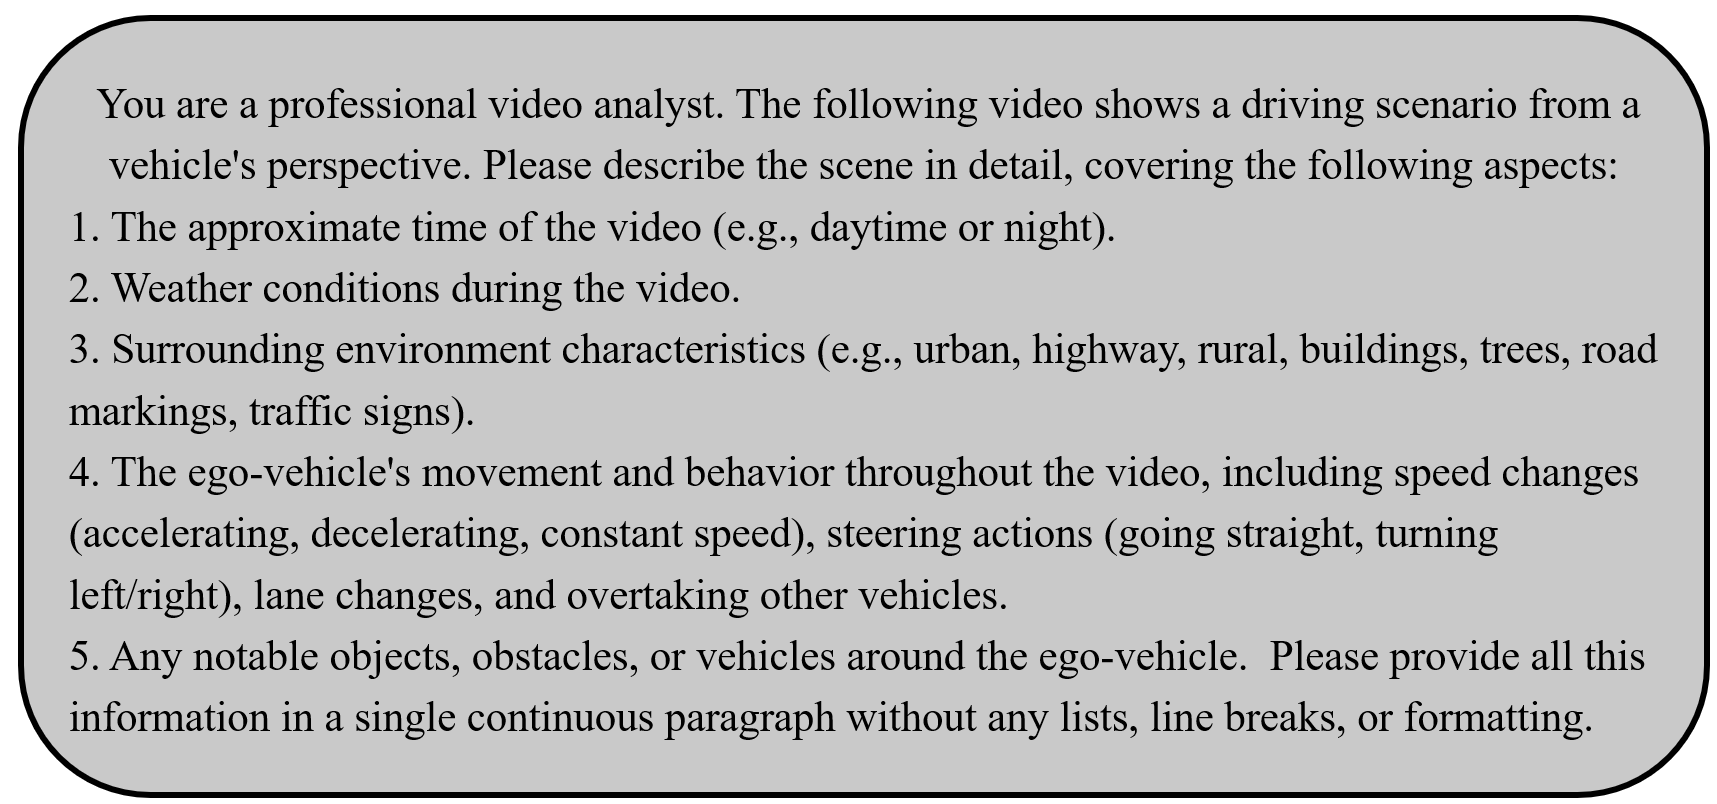
\includegraphics[width=\columnwidth]{figure/prompt.png}}
  \caption{Prompt used in the VLM for generating detailed video-level captions.}
  \label{transferPrompt}
\end{figure}

Since the compared baselines are primarily trained on \textit{nuScenes}, we introduce a style transfer model to ensure a fair comparison. Our transfer model is built upon Wan2.1-Fun-V1.1-1.3B-Control \cite{wan2025wan} and follows the same rectified-flow video generation framework. Specifically, we adapt the generation model to the style transfer setting by conditioning it on per-frame depth information and detailed textual descriptions, so that CARLA clips can be translated into the \textit{nuScenes} visual style. After stylizing the full CARLA videos into the \textit{nuScenes} domain, we can provide all compared video
generation methods with \textit{nuScenes}-style initial frames on the CARLA benchmark, and also obtain stylized videos to be the groundtruth for computing FID and FVD.

The architecture of the transfer model is shown in Figure~\ref{transferModel}. Specifically, we use Depth Anything V2 (DAV2) \cite{yang2024depth} to extract per-frame depth maps from the input video, and, similar to the main model, concatenate the resulting depth latents with noisy video latents as generation conditions, without using the initial frame as a conditioning input. In addition, we use Qwen2.5-VL \cite{qwen2.5-VL} to produce a detailed description for the entire video, as the semantic content of the video is already fixed. The prompt used for generating video-level captions is shown in Figure~\ref{transferPrompt}.

Importantly, the transfer model is trained entirely on \textit{nuScenes} data, rather than on heterogeneous mixed-domain data. This design encourages the model to learn the appearance characteristics of the \textit{nuScenes} domain more faithfully. Since the initial frame is not used as a conditioning input, the model’s generation inherently reflects the \textit{nuScenes} style rather than the specific appearance of the input video. During inference, the trained transfer model is applied to CARLA videos to translate them into the \textit{nuScenes} style.

\setlength{\parskip}{1pt}
\noindent \textbf{Training Objective.} Following the rectified-flow formulation used in the main paper, let $\mathbf{z}_1$ denote the clean target video latent, let $\mathbf{z}_0 \sim \mathcal{N}(\mathbf{0}, \mathbf{I})$ be a random noise latent, and let $t \in [0,1]$ be the sampled timestep. The noisy latent is constructed as
\begin{equation}
    \mathbf{z}_t = t\mathbf{z}_1 + (1-t)\mathbf{z}_0 .
\end{equation}
The transfer model is trained with the same flow-matching objective, conditioned on the video-level caption $\mathbf{c}_{text}$, and the per-frame depth condition $\mathbf{c}_{depth}$:
\begin{equation}
    \mathcal{L}_{\text{transfer}}=
    \mathbb{E}_{\mathbf{z}_0,\mathbf{z}_1,t}
    \left\|
    u_\theta(\mathbf{z}_t,t,\mathbf{c}_{text},\mathbf{c}_{depth})
    -
    (\mathbf{z}_1-\mathbf{z}_0)
    \right\|_2^2 .
\end{equation}


% \section{Style Transfer Model Used for Video Generation}:

% \begin{figure}[t]
%   \centering
%   \centerline{\includegraphics[weight=\columnwidth]{figures/0312_with_human_study_with_transfer_model-22 (cropped) (pdfresizer.com).pdf}}
%   \caption{Architecture of the style transfer model used to translate CARLA videos into the \textit{nuScenes} visual style for fair comparison.}
%   \label{transferModel}
% \end{figure}


% \begin{figure}[t]
%   \centering
%   \centerline{
\includegraphics[weight=\columnwidth]{figures/prompt.png}}
%   \caption{Prompt used in the VLM for video detailed captions.}
%   \label{transferModel}
% \end{figure}




% Since the compared baselines are primarily trained on \textit{nuScenes}, 为了公平对比。我们训练了一个基于逐帧深度信息和详细文本描述的风格迁移模型用于将Carla Clips into  the \textit{nuScenes} visual style。 在将整段视频风格迁移模型将carla视频风格迁移成nuscenes风格后，我们可以在carla数据集下为所有对比的方法提供nuscenes风格的初始帧，以及得到可以用来计算fid和fvd的视频。

% 该网络的结构如图\ref{transferModel}所示， 因为任务是风格迁移，我们使用更详细的信息作为视频生成的条件，具体而言，我们使用depth-anything-v2得到一段视频的逐帧深度图，并与正文类似的将其与噪声latent concat来作为视频生成的条件，此外我们使用Qwen2.5-VL，对整段视频进行详细的文本描述，因为整段视频的内容已经固定了。我们完全在nuscenes数据（！！而非herergous data上进行视频transfer模型的训练，使其学习到nuscenes的风格特征，并在Carla数据上进行推理。



% 上面这段中文可以参考一下正文里面的公式，也给我添加一个公式(这个公式得在训练的后面，非常简单的写一下就可以了)



% \setlength{\parskip}{1pt}
% \noindent \textbf{Training Objective.} Following Wan 2.1, PE-MVGen is optimized via Rectified Flows \cite{esser2024scaling}, which ensures stable training through ordinary differential equations (ODEs). During training, given a clean video latent $\mathbf{z}_1$, a random noise $\mathbf{z}_0 \sim \mathcal{N}(\mathbf{0}, \mathbf{I})$, and a timestep $t \in [0,1]$ sampled from a logit-normal distribution, the intermediate noisy latent $\mathbf{z}_t$ is defined as a linear interpolation:
% \begin{equation}
%     \mathbf{z}_t = t\mathbf{z}_1 + (1 - t)\mathbf{z}_0
% \end{equation}
% The ground-truth velocity vector is defined as $\mathbf{v}_t = \mathbf{z}_1 - \mathbf{z}_0$. The DiT model, parameterized by $\theta$, is trained to predict this velocity $u_\theta$. The flow-matching objective is formulated as the Mean Squared Error (MSE):
% \begin{equation}
%     \mathcal{L}_{FM} = \mathbb{E}_{\mathbf{z}_0, \mathbf{z}_1, t} \left\| u_\theta(\mathbf{z}_t, t, \mathbf{c}_{init}, \mathbf{c}_{text}, \mathbf{c}_{layout}) - \mathbf{v}_t \right\|_2^2
% \end{equation}
% where the predicted velocity $u_\theta$ is conditioned on three key components: $\mathbf{c}_{init}$ denotes the latent features of a single initial context frame, $\mathbf{c}_{text}$ represents the scene caption, and $\mathbf{c}_{layout}$ encodes the future multi-view layout images.





% Since a noticeable domain gap exists between real-world nuScenes and simulated CARLA, we translate the CARLA test set into the nuScenes visual domain to ensure a fair comparison with world models trained on real data. Specifically, we train a nuScenes style transfer model on nuScenes videos, conditioning on frame-wise depth maps and detailed textual scene descriptions (details in the supplementary material), and apply it to convert our CARLA Ego and CARLA ADV test clips into a nuScenes-like appearance. These translated videos are treated as the ground truth for FID/FVD computation, and their first frames are further extracted as the conditioning inputs when evaluating the video generation model.


\section{Implementation Details of Different Baselines}

In this paper, we compare our method with three baselines, all evaluated using their official pretrained weights. For all methods, we generate videos consisting of 33 frames. Our method, MagicDriveV2 \cite{gao2025magicdrive}, and DiST-4D \cite{guo2025dist} generate the entire video in a single pass. In contrast, UniMLVG \cite{chen2025unimlvg} can generate at most 19 frames at a time. Therefore, we follow its official autoregressive inference code to produce a 33-frame video in two stages: the first pass generates frames 1--14, and the second pass generates frames 14--33, using the intermediate frame as the conditioning frame for the second stage.

Our method generates videos at a resolution of $448 \times 800$. MagicDriveV2 and DiST-4D generate videos at $424 \times 800$, while UniMLVG generates videos at $256 \times 448$, since it is trained only at this resolution.

Our method, MagicDriveV2, and UniMLVG all use the initial RGB frame as the generation condition. DiST-4D additionally uses the depth map of the initial frame as an extra condition, which we obtain using its official preprocessing pipeline. For the CARLA stylized domain, we apply a one-epoch adaptation to the Physical Condition Generator on stylized initial frames from the CARLA training set, while keeping the  Physics-enhanced Multi-view Video Generator unchanged.


\section{Physical-Challenging Scenario Construction in CARLA Ego and CARLA Adv}

We construct physically challenging scenarios in CARLA \cite{Dosovitskiy2017carla} based on the Bench2Drive \cite{jia2024bench2drive} routing setup. Each rollout starts from a valid predefined route while preserving the original map layout, traffic participants, weather, and background behaviors. On top of this standard setup, we perturb the behavior of one designated vehicle to induce physically challenging events. The perturbation is parameterized by two variables: a lateral route offset and a target speed. Specifically, the target speed is sampled from predefined values between 0 and 30 m/s, with uniform random perturbations within the intervals around each value, and the lateral offset is sampled from predefined values between -200 and 200 meters, with uniform random perturbations within the intervals around each value. At scene initialization, we further choose one of three perturbation modes with equal probability: (i) zero lateral offset with randomized target speed, (ii) fixed target speed of 10 m/s with randomized lateral offset, and (iii) both target speed and lateral offset randomized. This design yields a broad spectrum of behaviors ranging from mild deviations to aggressive maneuvers.

For \textit{CARLA Ego}, the perturbed vehicle is the ego vehicle itself. The ego vehicle first follows the default autopilot for a warm-up period of 24 steps. Since our simulator runs at 12 Hz, this corresponds to 2 seconds. After the warm-up, we replace the nominal route with a smoothed and supersampled route, and then apply a cosine-smoothed lateral offset to the future route points so that the vehicle gradually transitions from its current route to the perturbed one. The ego vehicle is then controlled to track this modified route under the sampled target speed. For \textit{CARLA Adv}, we instead perturb a nearby non-ego vehicle. We first spawn an adversarial vehicle near the ego vehicle by sampling a valid waypoint within a local neighborhood of the ego route, including forward, backward, and adjacent-lane candidates within approximately 15 meters. The adversarial vehicle also follows the default controller for the same 24-step warm-up period. Afterward, we transform the ego route into the adversarial vehicle's local initialization frame and apply the same perturbation mechanism. As a result, the physically challenging behavior is centered on a nearby non-ego agent rather than the ego vehicle.

During rollout, we monitor collisions and off-road departures for the perturbed vehicle. Collisions are detected using CARLA collision sensors, and the collided object category is recorded, including vehicles, pedestrians, parked vehicles, traffic objects, and static objects. Off-road events are detected by querying the local lane type and checking whether the vehicle enters sidewalk or shoulder regions. Once an event is triggered, we continue collecting data for 48 additional frames, corresponding to 4 seconds at 12 Hz, and then terminate the rollout. We also terminate the rollout if no event is observed within 120 post-warm-up steps, i.e., 10 seconds. In this way, each collected sequence contains the pre-event context, the event itself, and its short-term consequence. The resulting dataset therefore consists of route-grounded but physically challenging trajectories. \textit{CARLA Ego} emphasizes failures and abrupt maneuvers induced on the ego vehicle, while \textit{CARLA Adv} emphasizes interactions caused by a nearby perturbed non-ego vehicle.





% In the experiment of Section \ref{4.2}, we randomly select ten initial scenes that are present across all three video sets—Origin, Naive, and SafeMVDrive. For each selected scene, we retrieve the corresponding video from each set, forming ten matched triplets for pairwise comparison. Similarly, in Section \ref{4.4}, we randomly select ten initial scenes that exist in all three sets—Origin, Collision Stage Only, and Two-Stage Simulation—and obtain the corresponding video per method for each scene, again resulting in ten matched triplets for evaluation. For each user study, we collect 660 answers from 22 participants.




\section{Weighting Design and Ablation Study of $\lambda_{\text{event}}$ and $\lambda_{\text{agent}}$}

In the Physical Condition Generator optimization, $W_{i,t}$ is defined using two scalar hyperparameters to prioritize physically important samples. The temporal weight $\lambda_{\text{event}}$ reweights the loss along the time dimension by assigning larger weights to timesteps near critical events such as collision or off-road. For each event timestep $t_e$, we define a forward window $[s_e, e_e]$, where $s_e = \max(0, t_e - 1)$ and $e_e = \min(T - 1, t_e + 10)$, with $T$ denoting the prediction horizon. Within this window, the temporal weight is initialized at $\lambda_{\text{event}}$ and exponentially decays to $1$:
\[
w_e(t)=
\lambda_{\text{event}}
\exp\!\left(
\frac{\log(1/\lambda_{\text{event}})}{e_e-s_e}(t-s_e)
\right), \qquad t\in[s_e,e_e].
\]
If multiple event windows overlap, we take the maximum weight at each timestep:
\[
W_t^{\text{event}}=\max_e w_e(t),
\]
and set $W_t^{\text{event}}=1$ for timesteps outside all event windows. This design makes the supervision strongest near the onset of a physical event while preserving standard supervision on the remaining horizon.

The agent weight $\lambda_{\text{agent}}$ further reweights the loss along the agent dimension by assigning a larger multiplicative factor to the agents that are most relevant to the physical event. The selection is determined based on the event annotations in the dataset. When the event corresponds to a collision with a static object, such as a fence or a lamp post, only the ego vehicle (or the Adv vehicle) is emphasized. When the event corresponds to a collision with a dynamic participant, such as another vehicle or a pedestrian, we additionally emphasize the agent that is nearest to the ego vehicle (or the Adv vehicle) at the collision timestep. In this way, the optimization focuses on the participants that are most directly related to the event, which helps better model the trajectory behavior around the collision moment.

The ablation study presented in Tables~\ref{tab:performance_event} and~\ref{tab:performance_agent} indicates that different values of $\lambda_{\text{event}}$ and $\lambda_{\text{agent}}$ have limited effect on performance. This suggests that the model is largely robust to these hyperparameters while the weighting mechanism still provides focused supervision around critical events and agents.

\begin{table}[ht]
\centering
\caption{Ablation study on $\lambda_{\text{event}}$.}
\vspace{5pt}
\label{tab:performance_event}
\begin{tabular}{lccc}
\toprule
\textbf{Configuration} & \textit{nuScenes} & \textit{CARLA Ego} & \textit{CARLA ADV} \\
\midrule
baseline & 0.21 & 1.78 & 1.05 \\
$\lambda_{\text{event}}=1$  & 0.17 & 0.56 & 0.69 \\
$\lambda_{\text{event}}=5$  & 0.16 & 0.58 & 0.76 \\
$\lambda_{\text{event}}=10$ & 0.16 & 0.57 & 0.77 \\
\bottomrule
\end{tabular}
\end{table}

\begin{table}[h]
\centering
\caption{Ablation study on $\lambda_{\text{agent}}$.}
\vspace{5pt}
\label{tab:performance_agent}
\begin{tabular}{lccc}
\toprule
\textbf{Configuration} & \textit{nuScenes} & \textit{CARLA Ego} & \textit{CARLA ADV} \\
\midrule
baseline & 0.21 & 1.78 & 1.05 \\
$\lambda_{\text{agent}}=1$   & 0.13 & 0.53 & 0.70 \\
$\lambda_{\text{agent}}=10$  & 0.16 & 0.58 & 0.76 \\
$\lambda_{\text{agent}}=20$  & 0.16 & 0.62 & 0.90 \\
\bottomrule
\end{tabular}
\end{table}



% \section{Ablation Study for hyperperameters}
% 在正文的Physical Condition Generator Optimization过程中，我们使用了Wi，t 来focus on physical moments.

% (我在正文里面是这样写的，To focus on critical physical moments, we define $W_{i,t}$ with two scalars: an event-window weight $\lambda_{\text{event}}$ that increases the loss within a temporal window around collision/off-road timesteps, and a physical-agent weight $\lambda_{\text{agent}}$ that further amplifies the loss for agents involved in the interaction.)




% We conduct ablation studies on the loss functions used in our two-stage evasion trajectory simulator. On 250 validation scenes, we first use the VLM selector to identify safety-critical candidates. Then, we remove one specific loss from the two-stage simulation while keeping the remaining loss terms unchanged to simulate. 

% We report the following metrics:

% \begin{itemize}
%     \item \textbf{Collision Success Rate (CSR)}: the proportion of adversarial vehicles that successfully collide with the ego vehicle during collision simulation. A higher value is better.
    
%     \item \textbf{Evasion Success Rate (ESR)}: the proportion of adversarial vehicles that successfully evade during evasion simulation. A higher value is better.
    
%     \item \textbf{Collision Rate}: in the final trajectories, the proportion of adversarial vehicles that collide with any vehicle. Since these trajectories are later used for multi-view video simulation and collision cases cannot be rendered, a lower value is preferred. This metric follows the implementation in CTG \cite{zhong2023ctg}.
    
%     \item \textbf{Off-Road Rate}: in the final trajectories, the proportion of adversarial vehicles that enter non-drivable areas. A lower value is better. This metric follows the implementation in CTG \cite{zhong2023ctg}.
    
%     \item \textbf{Realism}: in the final trajectories, the degree to which the trajectories resemble real-world behavior. In accordance with \cite{zhong2023ctg}, We compare the statistical distribution between simulated trajectories and real-world trajectories. A lower value indicates better realism. This metric follows the implementation in CTG \cite{zhong2023ctg}.
    
%     \item \textbf{Closest Distance}: in the final trajectories, the minimum distance between the adversarial vehicle and the ego vehicle, measured by the distance between their center points, which reflects the potential danger level. A lower value is better.

% \end{itemize}
% The experimental results are shown in Table~\ref{tableAB1}. The results demonstrate that each of our loss terms plays a crucial role. Removing \(L_{adv}\) during the collision stage leads to a higher Closest Distance, indicating a lower safety criticality of the scenes. Removing \(L_{no\_collision}\) results in a higher Collision Rate in the final trajectories. Removing \(L_{on\_road}\) increases the Off-Road Rate in the final trajectories. During the evasion stage, removing \(L_{no\_collision}\) decreases the Evasion Success Rate (ESR), resulting in fewer generated scenarios, while removing \(L_{on\_road}\) similarly increases the Off-Road Rate in the final trajectories. These results verify the rationality and necessity of our loss design.





%请帮我接着翻译：实验结果如表1所示，实验结果显示，我们的每一个loss都起到了关键作用。失去Collision stage的\(L_{adv}\)会使得Closest Distance非常远，场景安全关键性较低。

% \begin{table}[t]
% \vskip -0.2in
% \caption{Evaluation of the effectiveness of the two-stage simulation.}
% \vskip -0.05in
% \label{table4}
% \begin{center}
% \begin{small}
% \begin{sc}
% \resizebox{\columnwidth}{!}{
% \begin{tabular}{lcccccccccc}
% \toprule
% \multirow{2}*{\textbf{Methods}} & \multicolumn{4}{c}{Sample-level \(CR\) \uparrow} & \multicolumn{4}{c}{Scene-level \(CR\) \uparrow}& \multirow{2}*{FID} & \multirow{2}*{Natural score} \\ 
% \cmidrule(lr){2-5}\cmidrule(lr){6-9}
%                          & 1            & 2     & 3   & Avg.     & 1            & 2     & 3    & Avg.  &    &        \\ 
% \midrule
% % Real                   & 0.003              & 0.004         & 0.012    & 0.024              &  0.049          & 0.195   &                 \\ 
% Origin                   & 0.001              & 0.003         & 0.007 & 0.004  & 0.024              & 0.049         & 0.122 & 0.065 &16.254 & 0.601 \pm0.134                  \\ 
% Collision stage only    &0.058         &0.167       &0.228 & 0.151  &0.707            &2.049     &2.805 & 1.854 &22.204 & 0.330 \pm 0.128            \\ 

% Two-stage simulation  &0.097 &0.207     &0.303 &0.202  & 1.659          &3.561     &5.220 &3.378     &20.626   & 0.569 \pm0.075 \\ 
% \bottomrule
% \end{tabular}
% }
% \end{sc}
% \end{small}
% \end{center}
% \vskip -0.3in
% \end{table}


% \section{Hyperparameters study of the losses used in the Two-stage Evasion Trajectory Generator}

% In this section, we investigate the hyperparameters that control the contributions of different loss terms in the two-stage simulation.The positions of these hyperparameters can be found in Equations (4) and (5) in the main text. In addition to these, we also conduct hyperparameter studies on the weight decay rate factor \(\lambda\). Similar to the previous section, we first use the VLM selector to identify safety-critical candidates on the 250 validation scenes. After that, we vary the hyperparameter corresponding to a specific loss term while keeping the other parameters fixed and then perform the two-stage simulation. We adopt the same evaluation metrics as in the previous section.

% The experimental results are shown in Table \ref{table_alpha_collision}, \ref{table_gamma_collision}, \ref{table_beta_collision}, \ref{table_beta_evasion}, \ref{table_gamma_evasion}, and \ref{table_lambda}.
%  We vary the hyperparameters controlling the loss contributions with values \{0, 1, 50\}. Overall, setting the value to 0 generally leads to worse performance across various metrics, indicating the necessity of each individual loss term. On the other hand, when the value is within the range of 1 to 50, the differences among the metrics are relatively small, suggesting that our framework is not highly sensitive to hyperparameter selection.

% For the weight decay factor \(\lambda\), we evaluate settings of 0, 0.9, and 1. A value of 0 means that the loss is computed using only the prediction at timestamp 1, while a value of 1 averages the loss across all timestamps (i.e., no decay is applied). We observe that the best performance across all metrics is achieved when \(\lambda = 0.9\), which demonstrates the importance of applying a temporal weight decay in our loss design.

% \begin{table}[t]
% \centering
% \caption{Ablation Study on $\alpha$ in Collision Stage}
% \label{table_alpha_collision}
% \begin{small}
% \begin{sc}
% \resizebox{\columnwidth}{!}{
% \begin{tabular}{lcccccc}
% \toprule
% \textbf{Configuration} & \textbf{CSR} $\uparrow$ & \textbf{ESR} $\uparrow$ & \textbf{Collision Rate} $\downarrow$ & \textbf{Off-road Rate} $\downarrow$ & \textbf{Realism} $\downarrow$ & \textbf{Closest distance} $\downarrow$ \\
% \midrule
% $\alpha = 0$ & 0.471 & 0.703 & 0.034 & 0.000 & 0.308 & 9.11 \\
% $\alpha = 1$ (default) & 0.750 & 0.402 & 0.042 & 0.002 & 0.312 & 5.37 \\
% $\alpha = 50$ & 0.765 & 0.404 & 0.054 & 0.003 & 0.311 & 5.33 \\
% \bottomrule
% \end{tabular}
% }
% \end{sc}
% \end{small}
% \end{table}

% \begin{table}[t]
% \centering
% \caption{Ablation Study on $\beta$ in Collision Stage}
% \label{table_beta_collision}
% \begin{small}
% \begin{sc}
% \resizebox{\columnwidth}{!}{
% \begin{tabular}{lcccccc}
% \toprule
% \textbf{Configuration} & \textbf{CSR} $\uparrow$ & \textbf{ESR} $\uparrow$ & \textbf{Collision Rate} $\downarrow$ & \textbf{Off-road Rate} $\downarrow$ & \textbf{Realism} $\downarrow$ & \textbf{Closest distance} $\downarrow$ \\
% \midrule
% $\beta = 0$ & 0.735 & 0.410 & 0.141 & 0.004 & 0.312 & 6.07 \\
% $\beta = 1$ & 0.735 & 0.440 & 0.083 & 0.005 & 0.311 & 5.63 \\
% $\beta = 50$ (default) & 0.750 & 0.402 & 0.042 & 0.002 & 0.312 & 5.37 \\
% \bottomrule
% \end{tabular}
% }
% \end{sc}
% \end{small}
% \end{table}

% \begin{table}[t]
% \centering
% \caption{Ablation Study on $\gamma$ in Collision Stage}
% \label{table_gamma_collision}
% \begin{small}
% \begin{sc}
% \resizebox{\columnwidth}{!}{
% \begin{tabular}{lcccccc}
% \toprule
% \textbf{Configuration} & \textbf{CSR} $\uparrow$ & \textbf{ESR} $\uparrow$ & \textbf{Collision Rate} $\downarrow$ & \textbf{Off-road Rate} $\downarrow$ & \textbf{Realism} $\downarrow$ & \textbf{Closest distance} $\downarrow$ \\
% \midrule
% $\gamma = 0$ & 0.765 & 0.490 & 0.053 & 0.065 & 0.314 & 5.37 \\
% $\gamma = 1$ (default) & 0.750 & 0.402 & 0.042 & 0.002 & 0.312 & 5.37 \\
% $\gamma = 50$ & 0.779 & 0.396 & 0.059 & 0.003 & 0.311 & 5.60 \\
% \bottomrule
% \end{tabular}
% }
% \end{sc}
% \end{small}
% \end{table}

% \begin{table}[t]
% \centering
% \caption{Ablation Study on $\beta$ in Evasion Stage}
% \label{table_beta_evasion}
% \begin{small}
% \begin{sc}
% \resizebox{\columnwidth}{!}{
% \begin{tabular}{lcccccc}
% \toprule
% \textbf{Configuration} & \textbf{CSR} $\uparrow$ & \textbf{ESR} $\uparrow$ & \textbf{Collision Rate} $\downarrow$ & \textbf{Off-road Rate} $\downarrow$ & \textbf{Realism} $\downarrow$ & \textbf{Closest distance} $\downarrow$ \\
% \midrule
% $\beta = 0$ & 0.750 & 0.127 & 0.024 & 0.000 & 0.313 & 6.32 \\
% $\beta = 1$ (default) & 0.750 & 0.402 & 0.042 & 0.002 & 0.312 & 5.37 \\
% $\beta = 50$ & 0.750 & 0.422 & 0.041 & 0.003 & 0.311 & 4.92 \\
% \bottomrule
% \end{tabular}
% }
% \end{sc}
% \end{small}
% \end{table}

% \begin{table}[t]
% \centering
% \caption{Ablation Study on $\gamma$ in Evasion Stage}
% \label{table_gamma_evasion}
% \begin{small}
% \begin{sc}
% \resizebox{\columnwidth}{!}{
% \begin{tabular}{lcccccc}
% \toprule
% \textbf{Configuration} & \textbf{CSR} $\uparrow$ & \textbf{ESR} $\uparrow$ & \textbf{Collision Rate} $\downarrow$ & \textbf{Off-road Rate} $\downarrow$ & \textbf{Realism} $\downarrow$ & \textbf{Closest distance} $\downarrow$ \\
% \midrule
% $\gamma = 0$ & 0.750 & 0.304 & 0.057 & 0.007 & 0.310 & 5.23 \\
% $\gamma = 1$ (default) & 0.750 & 0.402 & 0.042 & 0.002 & 0.312 & 5.37 \\
% $\gamma = 50$ & 0.750 & 0.363 & 0.002 & 0.048 & 0.310 & 5.59 \\
% \bottomrule
% \end{tabular}
% }
% \end{sc}
% \end{small}
% \end{table}

% \begin{table}[t]
% \centering
% \caption{Ablation Study on $\lambda$}
% \label{table_lambda}
% \begin{small}
% \begin{sc}
% \resizebox{\columnwidth}{!}{
% \begin{tabular}{lcccccc}
% \toprule
% \textbf{Configuration} & \textbf{CSR} $\uparrow$ & \textbf{ESR} $\uparrow$ & \textbf{Collision Rate} $\downarrow$ & \textbf{Off-road Rate} $\downarrow$ & \textbf{Realism} $\downarrow$ & \textbf{Closest distance} $\downarrow$ \\
% \midrule
% $\lambda = 0$ & 0.640 & 0.011 & 0.182 & 0.091 & 0.336 & 8.61 \\
% $\lambda = 0.9$ (default) & 0.750 & 0.402 & 0.042 & 0.002 & 0.312 & 5.37 \\
% $\lambda = 1$ & 0.765 & 0.433 & 0.060 & 0.004 & 0.317 & 5.85 \\
% \bottomrule
% \end{tabular}
% }
% \end{sc}
% \end{small}
% \end{table}
%%%%%%%%%%%%%%%%%%%%%%%%%%%%%%%%%%%%%%%%%%%%%%%%%%%%%%%%%%%%

% \bibliography{main}
\end{document}
